\section{TỔNG QUAN VỀ HỆ THỐNG}

\subsection{Bối cảnh kinh doanh (Business context)}
Trong bối cảnh ngành công nghiệp thực phẩm và dịch vụ ngày càng phát triển và cạnh tranh khốc liệt, việc ứng dụng công nghệ vào quản lý nhà hàng đã trở thành một xu hướng tất yếu. Hệ thống quản lý chuỗi nhà hàng là một giải pháp kỹ thuật số được thiết kế để hỗ trợ và tối ưu hóa các hoạt động vận hành hàng ngày của nhà hàng (đặc biệt là nhà hàng fine dining), từ đặt bàn, xử lý đơn hàng, thanh toán cho đến quản lý nhân sự. Một hệ thống quản lý chuỗi nhà hàng hiệu quả không chỉ giúp nâng cao trải nghiệm của khách hàng mà còn cải thiện hiệu suất làm việc của nhân viên và tối ưu hóa quản lý doanh thu.

% \subsubsection{Mục tiêu và phạm vi hệ thống}
% Hệ thống quản lý nhà hàng \textbf{\textit{Menu+}} được phát triển nhằm mục đích đơn giản hóa và nâng cao hiệu quả các hoạt động vận hành hàng ngày trong một nhà hàng fine dining. Các chức năng chính của \textbf{\textit{Menu+}} bao gồm:
% \begin{itemize}
%     \item \textbf{Đặt bàn trực tuyến và quản lý bàn}: Giúp khách hàng dễ dàng đặt chỗ và hỗ trợ nhân viên theo dõi trạng thái bàn một cách chính xác.
%      \item \textbf{Quản lý bàn}: Hỗ trợ nhân viên theo dõi trạng thái bàn (trống, đã đặt, đang phục vụ) và thực hiện các thao tác như chuyển bàn khi cần thiết.
%     \item \textbf{Xử lý đơn hàng}: Cho phép nhân viên nhập đơn hàng, tùy chỉnh theo yêu cầu của khách và gửi trực tiếp đến hệ thống hiển thị bếp (Kitchen Display System - KDS).
%     \item \textbf{Thanh toán và quản lý doanh thu}: Tích hợp các phương thức thanh toán đa dạng, tạo điều kiện thuận lợi cho cả khách hàng và nhà hàng.
%     \item \textbf{Quản lý quan hệ khách hàng (CRM) và nhân sự}: Lưu trữ thông tin khách hàng, quản lý lịch làm việc của nhân viên và cung cấp các báo cáo chi tiết về hoạt động kinh doanh.
% \end{itemize}
% \textbf{\textit{Menu+}} linh hoạt và thân thiện với người dùng đóng vai trò quan trọng trong việc giúp các nhà hàng, đặc biệt là những nhà hàng mới khởi nghiệp, mở rộng quy mô hoạt động một cách hiệu quả.

% \subsubsection{Ràng buộc kinh doanh (Business Constraint)}

% exclude

\subsubsection{Tổng quan hệ thống quản lý nhà hàng}

Dưới đây là mô tả tổng quan về các thành phần cấu thành hệ thống quản lý chuỗi nhà hàng, với các chức năng thiết yếu nhằm hỗ trợ việc vận hành và điều phối các hoạt động trong một chuỗi nhà hàng hiện đại. Những hệ thống con này đóng vai trò quan trọng trong việc tối ưu hóa hiệu quả công việc, nâng cao chất lượng dịch vụ và đảm bảo sự hoạt động trơn tru của toàn bộ chuỗi.

\begin{figure}[H]
	\centering
	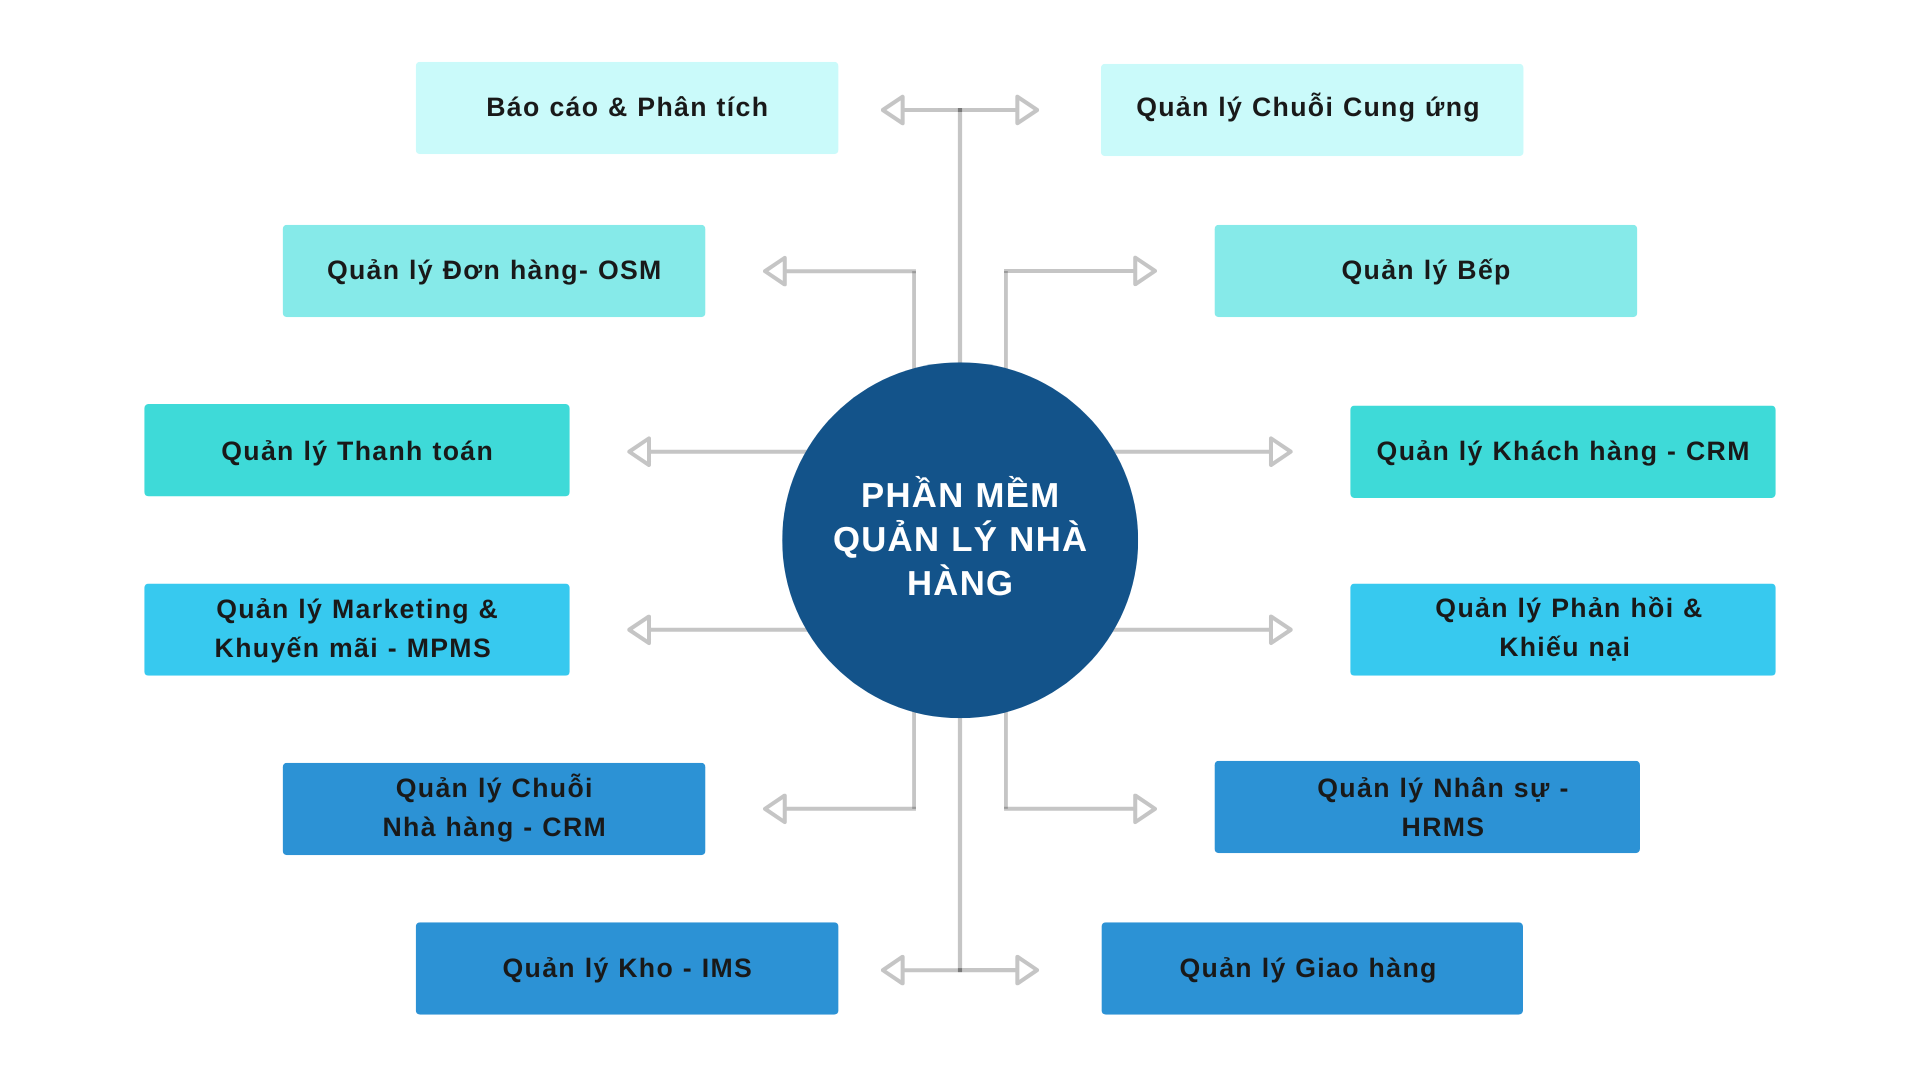
\includegraphics[width=15cm]{Images/so-do-he-thong.png}
	\vspace{0.5cm}
	\caption{Sơ đồ tổng quan về một hệ thống Quản lý Nhà hàng}
	\label{fig:my_label}
\end{figure}

\begin{itemize}
	\item \textbf{Hệ thống Quản lý Đơn hàng (Order Management System - OMS)}: Đóng vai trò quan trọng trong việc tiếp nhận và xử lý các đơn đặt món từ khách hàng. Khi khách hàng đặt món, thông tin đơn hàng sẽ được hệ thống OMS ghi nhận và phân phối đến các bộ phận liên quan trong nhà hàng, như bếp để chế biến món ăn, thu ngân để xử lý thanh toán, và đội ngũ giao hàng nếu có. Hệ thống OMS không chỉ giúp theo dõi tình trạng của từng đơn hàng mà còn quản lý các thông tin liên quan đến khách hàng và việc giao nhận món ăn. Đặc biệt, OMS sẽ giúp nhà quản lý theo dõi hiệu suất của đơn hàng và cập nhật kịp thời trạng thái để khách hàng có thể nhận được món ăn một cách nhanh chóng. Mọi thay đổi về đơn hàng sẽ được cập nhật liên tục để các bộ phận liên quan có thể xử lý ngay khi có sự thay đổi, ví dụ như khi khách hàng hủy đơn hoặc có yêu cầu thay đổi món.

	\item \textbf{Hệ thống Quản lý Bếp (Kitchen Management System - KMS)}: Tập trung vào việc quản lý quá trình chế biến món ăn từ khi nhận được đơn hàng từ OMS cho đến khi món ăn hoàn thành và sẵn sàng phục vụ khách. Thông qua KMS, nhà bếp có thể lên kế hoạch chế biến cho từng món ăn và theo dõi hiệu quả làm việc của từng đầu bếp. Mỗi đơn hàng sẽ được chia thành các công đoạn nhỏ để các nhân viên bếp dễ dàng theo dõi và thực hiện. Hệ thống này cũng đóng vai trò trong việc quản lý chất lượng món ăn, đảm bảo rằng món ăn được chế biến đúng quy trình và đạt tiêu chuẩn chất lượng. KMS cũng kết nối với các hệ thống khác như Inventory Management System (IMS) để tự động kiểm tra và yêu cầu bổ sung nguyên liệu khi kho hàng thiếu hụt.

	\item \textbf{Hệ thống Quản lý Kho (Inventory Management System - IMS)}: Quản lý và giám sát tình trạng nguyên liệu trong kho của các chi nhánh nhà hàng. IMS giúp nhà quản lý kiểm soát số lượng nguyên liệu, hạn sử dụng và các mặt hàng còn lại trong kho để đảm bảo rằng luôn có đủ nguyên liệu cho việc chế biến món ăn. Hệ thống này sẽ tự động thông báo khi lượng nguyên liệu sắp hết hoặc sắp hết hạn sử dụng, giúp bộ phận kho có thể lên kế hoạch nhập hàng bổ sung từ các nhà cung cấp. IMS không chỉ giúp đảm bảo việc cung cấp nguyên liệu kịp thời cho KMS, mà còn giúp giảm thiểu tình trạng thiếu hụt nguyên liệu, qua đó đảm bảo việc phục vụ khách hàng không bị gián đoạn. Hệ thống này cũng giúp tối ưu hóa việc sử dụng nguyên liệu, giảm lãng phí và giúp duy trì chi phí vận hành hợp lý.

	\item \textbf{Hệ thống Quản lý Thanh toán (Payment Management System - PMS)}: Chịu trách nhiệm xử lý tất cả các giao dịch thanh toán của khách hàng sau khi món ăn được giao đến bàn hoặc giao tận nơi. Khi món ăn hoàn thành và khách hàng chuẩn bị thanh toán, hệ thống PMS sẽ tự động tính toán giá trị đơn hàng, bao gồm thuế, chiết khấu, và các khoản phí khác nếu có. Hệ thống này hỗ trợ nhiều phương thức thanh toán khác nhau, từ tiền mặt, thẻ tín dụng, thẻ ghi nợ, cho đến các phương thức thanh toán trực tuyến. Sau khi thanh toán hoàn tất, PMS sẽ in hóa đơn cho khách và cập nhật dữ liệu doanh thu vào hệ thống tài chính. Hệ thống này cũng đồng bộ hóa dữ liệu với các hệ thống báo cáo để nhà quản lý có cái nhìn tổng quan về tình hình tài chính của từng chi nhánh. PMS còn có khả năng theo dõi và phân tích các xu hướng chi tiêu của khách hàng để đưa ra các chiến lược giá hợp lý và tăng trưởng doanh thu.

	\item \textbf{Hệ thống Quản lý Nhân sự (Human Resource Management System - HRMS)}: Quản lý thông tin nhân viên, lịch làm việc và hiệu suất công việc của các nhân viên trong chuỗi nhà hàng. Hệ thống này theo dõi số giờ làm việc, ca làm việc của nhân viên, và các yếu tố liên quan đến chấm công, bảo hiểm, tiền lương. Ngoài ra, HRMS còn hỗ trợ việc phân công công việc cho các nhân viên bếp, thu ngân, và các bộ phận khác, giúp việc tổ chức công việc trở nên khoa học và hợp lý. Các tính năng như theo dõi kỳ nghỉ, đào tạo và phát triển nhân viên cũng được HRMS đảm bảo. Một trong những chức năng quan trọng của HRMS là giúp tối ưu hóa quy trình tuyển dụng, giúp tuyển chọn nhân viên phù hợp với yêu cầu công việc. Ngoài ra, HRMS còn hỗ trợ các bộ phận quản lý nhân sự của từng chi nhánh trong việc đánh giá hiệu suất làm việc và cải thiện chất lượng nhân sự.

	\item \textbf{Hệ thống Báo cáo \& Phân tích (Reporting \& Analytics System - R\&A)}: Quản lý có cái nhìn tổng quan về hiệu suất của toàn chuỗi nhà hàng. Hệ thống này thu thập và tổng hợp dữ liệu từ các hệ thống khác nhau như OMS, KMS, IMS, PMS và HRMS để tạo ra các báo cáo chi tiết. Những báo cáo này không chỉ về tình hình doanh thu, mà còn cung cấp các thông tin liên quan đến hiệu quả công việc của nhân viên, tình trạng kho nguyên liệu, mức độ hài lòng của khách hàng, và nhiều yếu tố khác. Thông qua phân tích dữ liệu, nhà quản lý có thể đưa ra những quyết định chiến lược giúp cải thiện quy trình hoạt động, tối ưu hóa chi phí và nâng cao chất lượng dịch vụ. Hệ thống cũng hỗ trợ tạo ra các báo cáo tài chính, giúp các chi nhánh có thể theo dõi doanh thu và chi phí một cách chi tiết.

	\item \textbf{Hệ thống Quản lý Chuỗi Cung ứng (Supply Chain Management System - SCM)}: Quản lý và điều phối mối quan hệ với các nhà cung cấp, đảm bảo nguồn nguyên liệu luôn được cung cấp đầy đủ và đúng chất lượng. SCM theo dõi tình trạng đơn hàng từ khi nguyên liệu được đặt hàng cho đến khi nhận được hàng và đưa vào kho. Hệ thống này không chỉ giúp kiểm soát chất lượng nguồn cung mà còn tối ưu hóa quá trình giao nhận nguyên liệu, giảm thiểu tình trạng thiếu hụt hoặc tồn đọng hàng hóa trong kho. Bằng cách kết hợp dữ liệu từ IMS và KMS, SCM có thể dự báo nhu cầu nguyên liệu cho các món ăn, từ đó có kế hoạch đặt hàng hiệu quả hơn.

	\item \textbf{Hệ thống Quản lý Khách hàng (Customer Relationship Management - CRM)}: Lưu trữ và quản lý thông tin của khách hàng, bao gồm các thông tin cá nhân, lịch sử đơn hàng và các thói quen tiêu dùng. Hệ thống CRM giúp nhà hàng không chỉ lưu giữ thông tin khách hàng mà còn tạo dựng mối quan hệ lâu dài với khách hàng thông qua các chương trình khách hàng thân thiết và các ưu đãi cá nhân hóa. Bằng cách phân tích dữ liệu từ CRM, nhà hàng có thể hiểu rõ hơn về nhu cầu và sở thích của khách hàng, từ đó đề xuất các món ăn phù hợp, tạo ra những trải nghiệm cá nhân hóa. Hệ thống này còn hỗ trợ việc gửi các thông báo về chương trình khuyến mãi, sự kiện đặc biệt, hoặc thông tin về các sản phẩm mới đến khách hàng, giúp duy trì và phát triển mối quan hệ với khách hàng cũ và thu hút khách hàng mới.

	\item \textbf{Hệ thống Quản lý Marketing \& Khuyến mãi (Marketing \& Promotion Management System)}: Lên kế hoạch, triển khai và theo dõi các chiến dịch marketing và chương trình khuyến mãi. Hệ thống này hỗ trợ việc tạo ra các chiến dịch quảng bá các món ăn, khuyến mãi theo mùa hoặc các chương trình giảm giá đặc biệt cho khách hàng. Marketing \& Promotion Management System cung cấp các công cụ để tạo mã giảm giá, quản lý các chương trình khuyến mãi và theo dõi hiệu quả của từng chiến dịch. Hệ thống này còn giúp phân tích dữ liệu khách hàng từ CRM, từ đó xác định đối tượng mục tiêu cho các chiến dịch marketing, giúp tăng tỷ lệ chuyển đổi và tối ưu hóa chi phí marketing. Ngoài ra, các chiến dịch và khuyến mãi cũng có thể được tích hợp với hệ thống thanh toán để khách hàng có thể dễ dàng sử dụng các ưu đãi khi thanh toán.

	\item \textbf{Hệ thống Quản lý Phản hồi \& Khiếu nại (Feedback \& Complaint Management System)}: Nhận và xử lý các phản hồi, khiếu nại từ khách hàng. Việc lắng nghe và giải quyết nhanh chóng các vấn đề của khách hàng giúp nhà hàng cải thiện chất lượng dịch vụ và tạo dựng lòng tin của khách hàng. Hệ thống này giúp theo dõi các khiếu nại về món ăn, thái độ phục vụ, không gian nhà hàng hoặc các vấn đề khác. Sau khi nhận được phản hồi hoặc khiếu nại từ khách hàng, hệ thống sẽ tự động phân loại và chuyển đến các bộ phận liên quan để xử lý, từ đó giúp khách hàng cảm thấy hài lòng hơn với dịch vụ của nhà hàng. Hệ thống này cũng có chức năng theo dõi các phản hồi tích cực để có thể ghi nhận và thưởng cho những nhân viên hoặc bộ phận có đóng góp xuất sắc.

	\item \textbf{Hệ thống Quản lý Chuỗi Nhà hàng (Chain Management System - CMS)}: Trung tâm quản lý tổng thể của chuỗi các chi nhánh nhà hàng. Hệ thống này giúp giám sát các hoạt động của tất cả các chi nhánh từ một hệ thống tập trung, bao gồm việc theo dõi doanh thu, tồn kho, nhân sự, cũng như các hoạt động vận hành khác của từng chi nhánh. CMS không chỉ giúp đồng bộ hóa các quy trình giữa các chi nhánh mà còn cung cấp các báo cáo tài chính và hoạt động chi tiết để hỗ trợ các quyết định quản lý chiến lược. Hệ thống này tích hợp dữ liệu từ các hệ thống khác như PMS, KMS, IMS, giúp nhà quản lý chuỗi có thể theo dõi tình trạng của từng chi nhánh và đưa ra các quyết định kịp thời để tối ưu hóa hoạt động của toàn chuỗi.

	\item \textbf{Hệ thống Quản lý Giao hàng (Delivery Management System)}: Quản lý các đơn hàng giao tận nơi, bao gồm việc điều phối các nhân viên giao hàng, theo dõi tình trạng đơn hàng và tối ưu hóa thời gian giao hàng. Hệ thống này giúp các nhân viên giao hàng nhận được thông tin đơn hàng một cách nhanh chóng, biết rõ địa chỉ giao hàng và các yêu cầu đặc biệt của khách hàng (nếu có). Hệ thống còn giúp theo dõi trạng thái của đơn hàng từ khi rời khỏi nhà hàng cho đến khi giao đến tay khách hàng, đồng thời cung cấp các công cụ để quản lý các tuyến đường giao hàng sao cho hiệu quả và tiết kiệm thời gian. Việc tích hợp hệ thống này với OMS giúp cập nhật trạng thái của đơn hàng cho khách hàng trong thời gian thực và đảm bảo dịch vụ giao hàng nhanh chóng, chính xác.
\end{itemize}

\subsubsection{Chính sách vận hành (Policy)}
Các nhà hàng hiện đại ngày nay thường áp dụng nhiều chính sách linh hoạt nhằm nâng cao chất lượng phục vụ và giảm thiểu các rủi ro trong kinh doanh. Các chính sách phổ biến được áp dụng có thể kể tới như sau:

\begin{itemize}
	\item \textbf{Đa dạng hóa phương thức thanh toán}: Chính sách này tập trung vào việc cung cấp đa dạng các hình thức thanh toán, như tiền mặt, thẻ tín dụng, ví điện tử và mã QR. Bên cạnh đó, các nhà hàng cũng triển khai hệ thống quản lý thanh toán tự động để rút ngắn thời gian xử lý, giảm thiểu sai sót và tăng trải nghiệm hài lòng của khách hàng. Chính sách này đã được các nhà hàng như \textit{Ngưu Phồn} và \textit{Cơm niêu Sài Gòn} áp dụng rất hiệu quả.

	\item \textbf{Yêu cầu đặt cọc khi đặt bàn}: Để giảm thiểu tổn thất khi khách hàng hủy đặt bàn vào phút chót hoặc không đến nhà hàng mà không báo trước, nhiều nhà hàng áp dụng chính sách yêu cầu khách hàng đặt cọc trước một khoản tiền nhất định, thường dao động từ 10\% đến 20\% tổng giá trị bàn tiệc. Khoản đặt cọc này sẽ được khấu trừ vào hóa đơn thanh toán hoặc bị giữ lại nếu khách hủy đặt bàn trễ hơn thời gian quy định. Một số nhà hàng áp dụng thành công chính sách này là \textit{Nhà Hàng Phúc Thành} và \textit{Vân Nghĩa Palace}.

	\item \textbf{Xác nhận đặt bàn trước ngày hẹn}: Chính sách này yêu cầu nhân viên nhà hàng chủ động liên hệ với khách hàng trước ngày đặt bàn để xác nhận lại thông tin và nhắc nhở khách đến đúng giờ. Điều này không chỉ giúp giảm tình trạng khách quên hay thay đổi kế hoạch mà không thông báo, mà còn giúp nhà hàng quản lý hiệu quả hơn trong việc chuẩn bị dịch vụ. Nhà hàng áp dụng tiêu biểu chính sách này là \textit{Nhà Hàng Phúc Thành}.

	\item \textbf{Chính sách hủy đặt bàn và hoàn tiền rõ ràng}: Các nhà hàng thường đưa ra quy định chi tiết về thời hạn hủy đặt bàn và mức phí áp dụng khi hủy. Điều này giúp khách hàng hiểu rõ trách nhiệm và quyền lợi của mình khi sử dụng dịch vụ, đồng thời tạo ra sự minh bạch và uy tín trong hoạt động kinh doanh. Chính sách này được áp dụng rõ ràng tại \textit{Nhà Hàng Ocean Bay Vũng Tàu}.

	\item \textbf{Điều kiện hủy đơn hàng}: Chính sách này quy định rõ ràng các điều kiện và thời điểm cụ thể khách hàng được phép hủy đơn hàng, thường là trước khi nhà hàng xác nhận và bắt đầu chuẩn bị món ăn. Điều này giúp nhà hàng giảm thiểu tổn thất về nguyên vật liệu và công sức chế biến không cần thiết. Một ví dụ cụ thể về chính sách này là tại nhà hàng \textit{Patyko}.

	\item \textbf{Phí hủy đơn hàng}: Để bảo vệ quyền lợi và giảm thiểu thiệt hại khi khách hàng hủy đơn sau khi nhà hàng đã bắt đầu chế biến, nhiều nhà hàng đặt ra quy định thu phí hủy hoặc không hoàn lại tiền đặt cọc trong một số trường hợp nhất định. Chính sách này nhằm bù đắp một phần chi phí nguyên vật liệu và nhân công đã bỏ ra. Điển hình trong việc áp dụng chính sách này là \textit{Nhà Hàng Khoái}.

	\item \textbf{Chính sách đổi trả sản phẩm}: Để đảm bảo quyền lợi khách hàng và duy trì chất lượng dịch vụ, các nhà hàng thường áp dụng chính sách đổi trả rõ ràng. Khách hàng được quyền đổi hoặc trả lại món ăn trong các trường hợp món bị lỗi, hỏng, không thể sử dụng hoặc không đảm bảo vệ sinh an toàn thực phẩm. Chính sách này giúp tạo dựng lòng tin và gia tăng uy tín của nhà hàng. Một số nhà hàng nổi bật áp dụng thành công chính sách này là \textit{Sườn Mười} và \textit{Nhà Hàng Khoái}.

\end{itemize}



\begin{table}[H]
	\centering
	\caption{Tổng hợp các chính sách, mô tả và tham khảo từ các nhà hàng hoặc hệ thống liên quan}
	\begin{tabular}{|p{4cm}|p{8cm}|p{4cm}|}
		\hline
		\textbf{Tên chính sách}             & \textbf{Mô tả}                                                                                                                                                                                       & \textbf{Nhà hàng áp dụng}             \\
		\hline
		Đa dạng hóa phương thức thanh toán  & Cung cấp nhiều phương thức thanh toán như tiền mặt, thẻ tín dụng, ví điện tử và mã QR, đồng thời áp dụng hệ thống quản lý thanh toán tự động để giảm thiểu sai sót và tăng tốc độ phục vụ.           & Ngưu Phồn, Cơm niêu Sài Gòn           \\
		\hline
		Yêu cầu đặt cọc khi đặt bàn         & Để giảm thiểu tình trạng khách hàng hủy bàn vào phút chót hoặc không đến mà không báo trước, nhiều nhà hàng yêu cầu khách đặt cọc trước một khoản tiền, thường khoảng 10-20\% tổng giá trị bàn tiệc. & Nhà Hàng Phúc Thành, Vân Nghĩa Palace \\
		\hline
		Xác nhận đặt bàn trước ngày hẹn     & Trước ngày đặt bàn, nhân viên nhà hàng nên gọi điện hoặc nhắn tin xác nhận lại với khách hàng để nhắc nhở và đảm bảo họ sẽ đến.                                                                      & Nhà Hàng Phúc Thành                   \\
		\hline
		Chính sách hủy và hoàn tiền rõ ràng & Nhà hàng cần quy định rõ ràng về thời hạn hủy đặt bàn và mức phí hủy, giúp khách hàng nắm rõ quyền lợi và trách nhiệm của mình.                                                                      & Nhà Hàng Ocean Bay Vũng Tàu           \\
		\hline
		Điều kiện hủy đơn hàng              & Quy định rõ ràng về thời điểm và điều kiện khách hàng có thể hủy đơn hàng, đại khái hơn là trước khi nhà hàng xác nhận và lên đơn hàng.                                                              & Patyko                                \\
		\hline
		Phí hủy đơn hàng                    & Áp dụng phí hủy hoặc không hoàn tiền đặt cọc nếu khách hủy sau một thời điểm nhất định, giúp bù đắp chi phí nguyên liệu và công sức chuẩn bị.                                                        & Nhà Hàng Khoái                        \\
		\hline
		Chính sách đổi trả sản phẩm         & Chấp nhận đổi, trả các sản phẩm bị lỗi, hỏng, không thể sử dụng hoặc không đảm bảo vệ sinh an toàn thực phẩm.                                                                                        & Sườn Mười, Nhà Hàng Khoái             \\
		\hline
	\end{tabular}
\end{table}

\subsection{Người dùng và mục đích hệ thống Menu+}

Mục đích của hệ thống quản lý nhà hàng \textbf{\textit{Menu+}} là cung cấp một giải pháp toàn diện nhằm tối ưu hóa và nâng cao hiệu quả các hoạt động vận hành hàng ngày trong một nhà hàng fine dining. Hệ thống được phát triển với mục tiêu hỗ trợ các nhóm người dùng chính trong nhà hàng, bao gồm khách hàng, thu ngân, quản lý, quản trị viên, bếp trưởng, nhân viên phục vụ và nhân viên vệ sinh.

\begin{figure}[H]
	\centering
	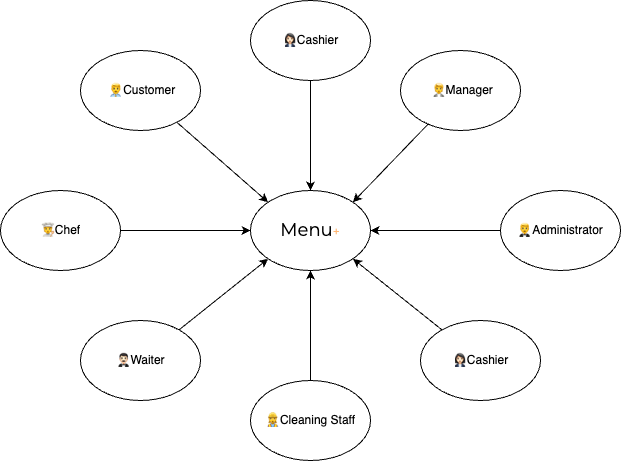
\includegraphics[width=15cm]{Images/OMS-Page-2.png}
	\vspace{0.5cm}
	\caption{Các người dùng trong hệ thống}
	\label{fig:my_label}
\end{figure}

% \begin{table}[h!]
% \centering
% \begin{tabular}{|p{3cm}|p{3cm}|p{9cm}|}
% \hline
% \textbf{Mã đối tượng} & \textbf{Tên} & \textbf{Mô tả} \\ \hline
% US-01 & Customer (Khách hàng) & Xem menu trực tuyến, đặt bàn hoặc order trực tiếp tại nhà hàng, thanh toán và sử dụng mã khuyến mãi. \\ \hline
% US-02 & Cashier (Thu ngân) & Thực hiện xác nhận thanh toán, gộp hoặc tách bill, hỗ trợ khách hàng sử dụng mã khuyến mãi, nhập số tiền nhận và tính tiền thối lại. \\ \hline
% US-03 & Manager (Quản lý) & Quản lý order, doanh thu, nhân sự, chia ca, thêm nhân sự mới, và điều hành chung hệ thống nhà hàng. \\ \hline
% US-04 & Administrator (Quản trị viên) & Quản lý và duy trì hệ thống, cấu hình menu, điều chỉnh các thông tin liên quan đến hệ thống chung. \\ \hline
% US-05 & Chef (Bếp trưởng) & Xem Kitchen Display System (KDS), xác nhận món ăn từ trạng thái "not ready", chuyển sang "cook" và cuối cùng là "ready to serve". \\ \hline
% US-06 & Waiter (Nhân viên phục vụ) & Giúp khách hàng đặt bàn, order món, lấy món ăn từ bếp, phục vụ món ăn, chuyển bàn, thực hiện self-order cho khách, cập nhật trạng thái món ăn là đã phục vụ. \\ \hline
% US-07 & Cleaning Staff (Nhân viên vệ sinh) & Dọn dẹp bàn ăn sau khi khách rời đi, cập nhật tình trạng bàn trên hệ thống để sẵn sàng phục vụ khách tiếp theo. \\ \hline
% \end{tabular}
% \caption{Bảng tổng hợp đối tượng và chức năng trong hệ thống quản lý nhà hàng}
% \label{tab:restaurant_objects}
% \end{table}

\textbf{Các chức năng chính của Menu+}

Hệ thống Menu+ bao gồm các chức năng chính giúp các nhóm người dùng trên thực hiện các công việc hàng ngày một cách hiệu quả và nhanh chóng:

\begin{itemize}


	\item Đặt bàn trực tuyến và quản lý bàn: Giúp khách hàng dễ dàng đặt chỗ và hỗ trợ nhân viên theo dõi trạng thái bàn (trống, đã đặt, đang phục vụ).

	\item Quản lý bàn: Cung cấp công cụ cho nhân viên theo dõi và quản lý bàn trong nhà hàng.

	\item Xử lý đơn hàng: Cho phép nhân viên nhập và gửi đơn hàng đến hệ thống Kitchen Display System (KDS) cho bếp.

	\item Thanh toán và quản lý doanh thu: Tích hợp các phương thức thanh toán đa dạng, tạo thuận tiện cho cả khách hàng và nhà hàng.

	\item Quản lý quan hệ khách hàng (CRM) và nhân sự: Lưu trữ thông tin khách hàng, quản lý lịch làm việc của nhân viên và cung cấp các báo cáo chi tiết về hoạt động kinh doanh.
\end{itemize}

\subsection{Đặc tả chức năng}
\begin{longtable}{|m{1.5cm}|m{3.5cm}|m{4.5cm}|m{5cm}|}
	\caption{Danh sách Người dùng Hệ thống} \label{tab:users}                                                                                                                                                                                                      \\
	\hline
	\textbf{Mã} & \textbf{Tên Người Dùng}    & \textbf{Vai Trò Thực Tế}                                  & \textbf{Mô Tả Ngắn}                                                                                                                                     \\
	\hline
	\endfirsthead

	\hline
	\textbf{Mã} & \textbf{Tên Người Dùng}    & \textbf{Vai Trò Thực Tế}                                  & \textbf{Mô Tả Ngắn}                                                                                                                                     \\
	\hline
	\endhead % Header cho các trang tiếp theo

	\hline
	\endfoot % Footer cho bảng

	\hline
	\endlastfoot % Footer cho trang cuối cùng

	US-01       & Quản lý nhà hàng           & Chủ nhà hàng hoặc người quản lý cấp cao                   & Quản lý tổng thể hoạt động, cấu hình hệ thống (giá bàn, \% đặt cọc, thời gian gọi bot), xem báo cáo toàn diện, quản lý nhân viên và thực đơn.           \\
	\hline
	US-02       & Nhân viên phục vụ          & Waiter/Waitress                                           & Sử dụng POS để nhận đơn hàng tại bàn, quản lý trạng thái bàn, xử lý thanh toán (bao gồm cả việc trừ tiền đặt cọc), tương tác với hệ thống bếp.          \\
	\hline
	US-03       & Nhân viên lễ tân           & Host/Hostess (Có thể là Nhân viên phục vụ đảm nhiệm)      & Quản lý sơ đồ tầng, trạng thái bàn, nhận và quản lý đặt chỗ trực tiếp hoặc qua điện thoại (ít tương tác hệ thống hơn khách hàng tự đặt).                \\
	\hline
	US-04       & Nhân viên bếp              & Chef, Cook, Kitchen Assistant                             & Tương tác chính với Màn hình hiển thị Bếp (KDS) hoặc máy in phiếu bếp để xem chi tiết đơn hàng (bao gồm món đặt trước) và cập nhật trạng thái chuẩn bị. \\
	\hline
	US-05       & Nhân viên thu ngân         & Cashier (Có thể là Nhân viên phục vụ hoặc Quản lý)        & Chịu trách nhiệm đóng/mở phiên POS, đối soát tiền mặt cuối ngày, xử lý các giao dịch thanh toán.                                                        \\
	\hline
	US-06       & Kế toán                    & Accountant/Bookkeeper                                     & Truy cập dữ liệu bán hàng đã được tổng hợp, báo cáo tài chính, quản lý công nợ (nếu có), đối soát doanh thu và tiền đặt cọc.                            \\
	\hline
	US-07       & Nhân viên (Chung)          & Bất kỳ nhân viên nào cần xem lịch làm việc                & Xem lịch làm việc cá nhân được phân công qua Employee Portal, có thể có quyền yêu cầu đổi ca hoặc báo nghỉ.                                             \\
	\hline
	US-08       & Khách hàng                 & Customer/Guest                                            & Tương tác qua giao diện web/app để đặt bàn, đặt món ăn trước, thanh toán đặt cọc, đặt hàng mang về hoặc giao hàng.                                      \\
	\hline
	US-09       & Nhân viên hỗ trợ/ Vận hành & Support/Operations Staff                                  & Tiếp nhận và xử lý các yêu cầu hỗ trợ từ khách hàng.                                                                                                    \\
	\hline
	US-10       & Quản trị viên Hệ thống     & System Administrator (Có thể là Quản lý nhà hàng hoặc IT) & Thực hiện các cấu hình kỹ thuật sâu, quản lý tích hợp (Shipday, Bot), quản lý tài khoản người dùng và phân quyền chi tiết.                              \\
	\hline
\end{longtable}

\newpage % Ngắt trang



\begin{longtable}{|m{2.5cm}|m{2.5cm}|m{5cm}|m{5cm}|}
	\caption{Phân công Chức năng theo Người dùng} \label{tab:user_function_map}                                                                                                                                                            \\
    \hline
	\textbf{Người dùng}                                     & \textbf{Mã chức năng} & \textbf{Tên chức năng}                                 & \textbf{Mô tả ngắn}                                                                         \\
	\hline
	\endfirsthead % Header cho các trang tiếp theo
	
    \hline
	\textbf{Người dùng}                                     & \textbf{Mã chức năng} & \textbf{Tên chức năng}                                 & \textbf{Mô tả ngắn}                                                                         \\
	\hline
	\endhead % Header cho các trang tiếp theo

	\midrule
	\endfoot % Footer cho bảng

	% \bottomrule
	% \endlastfoot % Footer cho trang cuối cùng

	% === US-01: Quản lý nhà hàng ===
	\multicolumn{4}{|l|}{\textbf{US-01: Quản lý nhà hàng}}                                                                                                                                                                                 \\ \hline
	\multirow{15}{=}[2pt]{US-01: Quản lý nhà hàng}          & FR-MD01-01            & Tạo ca làm việc                                        & Cho phép định nghĩa các ca làm việc mới (thời gian, vai trò, số lượng).                     \\
	                                                        & FR-MD01-02            & Gán nhân viên vào ca                                   & Chỉ định nhân viên cụ thể cho các vị trí trống trong ca làm việc.                           \\
	                                                        & FR-MD01-03            & Xem lịch biểu Gantt                                    & Hiển thị lịch làm việc dạng Gantt, lọc theo vai trò, xem theo ngày/tuần/tháng.              \\
	                                                        & FR-MD01-04            & (Kích hoạt) Phát hiện trùng lịch                       & Kích hoạt hệ thống kiểm tra trùng lịch khi gán nhân viên.                                   \\
	                                                        & FR-MD01-05            & Xuất bản và Thông báo lịch                             & Công khai lịch làm việc và kích hoạt gửi thông báo đến nhân viên.                           \\
	                                                        & FR-MD01-07            & Sao chép lịch tuần                                     & Sao chép nhanh lịch làm việc của một tuần sang tuần khác.                                   \\
	                                                        & FR-MD01-08            & Quản lý vai trò công việc                              & Định nghĩa các vai trò công việc trong nhà hàng.                                            \\
	                                                        & FR-MD01-10            & Xem lịch theo vai trò                                  & Lọc và xem lịch làm việc của các nhân viên theo vai trò cụ thể.                             \\ \cline{2-4}
	                                                        & FR-MD02-01            & Tạo Sản phẩm Mới (Món ăn/Đồ uống)                      & Thêm món ăn, đồ uống mới vào hệ thống (tên, giá, loại...).                                  \\
	                                                        & FR-MD02-02            & Chỉnh sửa Thông tin Sản phẩm                           & Cập nhật chi tiết sản phẩm đã có (giá, mô tả, ảnh...).                                      \\
	                                                        & FR-MD02-03            & Lưu trữ/Hủy kích hoạt Sản phẩm                         & Ẩn/Hiện sản phẩm khỏi các giao dịch mà không xóa hẳn.                                       \\
	                                                        & FR-MD02-04            & Quản lý Danh mục Sản phẩm POS                          & Tạo, sửa, xóa, sắp xếp các danh mục hiển thị trên POS.                                      \\
	                                                        & FR-MD02-05            & Định nghĩa Thuộc tính \& Giá trị (cho Biến thể)        & Định nghĩa các đặc tính (size, độ cay) và lựa chọn (S, M, L). (Có thể là US-10)             \\
	                                                        & FR-MD02-06            & Cấu hình Biến thể Sản phẩm                             & Áp dụng thuộc tính/giá trị vào sản phẩm gốc để tạo biến thể, cấu hình giá riêng.            \\
	                                                        & FR-MD02-07            & Thiết lập Loại Sản phẩm                                & Xác định loại sản phẩm (Consumable, Stockable, Service).                                    \\
	                                                        & FR-MD02-08            & Cấu hình Hiển thị trên POS                             & Đánh dấu sản phẩm bán trên POS và gán vào danh mục POS.                                     \\
	                                                        & FR-MD02-09            & Quản lý Hình ảnh Sản phẩm                              & Tải lên, thay thế, xóa hình ảnh đại diện cho sản phẩm.                                      \\
	                                                        & FR-MD02-10            & Cấu hình In Bếp/Hiển thị KDS                           & Chỉ định danh mục sản phẩm nào gửi đến máy in/KDS nào.                                      \\
	                                                        & FR-MD02-11            & Định nghĩa Sản phẩm Tùy chọn/Phụ thu                   & Tạo các sản phẩm nhỏ (Extra cheese) để dùng làm modifier trên POS.                          \\ \cline{2-4}
	                                                        & FR-MD03-11            & Cấu hình Tham số Đặt chỗ                               & Thiết lập giờ hoạt động, giới hạn khách, quy tắc đặt cọc, giá bàn...                        \\
	                                                        & FR-MD03-12            & Xem Danh sách Đặt chỗ                                  & Xem danh sách tổng hợp các lượt đặt chỗ và trạng thái.                                      \\
	                                                        & FR-MD03-13            & Xem Chi tiết Đặt chỗ                                   & Xem thông tin chi tiết của một lượt đặt chỗ cụ thể.                                         \\
	                                                        & FR-MD03-14            & Tạo/Sửa Đặt chỗ Thủ công                               & Tạo hoặc sửa đặt chỗ cho khách qua kênh offline (điện thoại...).                            \\
	                                                        & FR-MD03-15            & Quản lý Trạng thái Đặt chỗ                             & Thay đổi trạng thái đặt chỗ (Xác nhận, Đã đến, Hủy...).                                     \\
	                                                        & FR-MD03-16            & Xem Danh sách Món đặt trước                            & Xem các món cần chuẩn bị cho các đặt chỗ sắp tới.                                           \\ \cline{2-4}
	                                                        & FR-MD04-05            & Cấu hình Dịch vụ Bot Call                              & Cấu hình tham số tích hợp Bot Call (số ngày gọi, kịch bản, số hỗ trợ...). (Có thể là US-10) \\ \cline{2-4}
	                                                        & FR-MD05-01            & Mở phiên làm việc POS                                  & Bắt đầu phiên làm việc POS, nhập tiền mặt đầu ca. (Thường là US-05)                         \\
	                                                        & FR-MD05-13            & Đóng Phiên làm việc POS                                & Kết thúc phiên làm việc, tổng kết, đối chiếu tiền mặt. (Thường là US-05)                    \\
	                                                        & FR-MD05-14            & Chuyển bàn/Ghép bàn                                    & Di chuyển hoặc gộp đơn hàng giữa các bàn.                                                   \\
	                                                        & FR-MD05-15            & Hủy món/Hủy đơn (Void)                                 & Hủy bỏ món hoặc đơn hàng (có thể cần quyền quản lý).                                        \\ \cline{2-4}
	                                                        & FR-MD09-03            & Xem Báo cáo Doanh thu Phiên POS                        & Xem báo cáo tổng kết chi tiết của các phiên POS đã đóng.                                    \\
	                                                        & FR-MD09-04            & Xem Báo cáo Bán hàng theo Sản phẩm/Danh mục            & Xem thống kê số lượng, doanh thu theo từng món ăn/danh mục.                                 \\
	                                                        & FR-MD09-05            & Xem Báo cáo Hiệu suất Nhân viên (POS)                  & Xem doanh thu, số đơn hàng theo từng nhân viên POS.                                         \\
	                                                        & FR-MD09-06            & Xem Báo cáo Tiền đặt cọc                               & Xem báo cáo tổng hợp tình hình thu, sử dụng, mất cọc.                                       \\
	                                                        & FR-MD09-07            & Xem Báo cáo Doanh thu theo Loại hình                   & Phân tích doanh thu theo Eat-in, Takeout, Delivery.                                         \\
	                                                        & FR-MD09-08            & Xuất dữ liệu Báo cáo                                   & Xuất dữ liệu báo cáo ra file Excel/CSV.                                                     \\ \cline{2-4}
	                                                        & FR-MD10-04            & Cấu hình Chung của Hệ thống                            & Cấu hình thông tin công ty, logo, tiền tệ, email... (Có thể là US-10)                       \\
	                                                        & FR-MD10-05            & Cấu hình Tích hợp Bên thứ ba                           & Quản lý API keys cho Cổng thanh toán, Bot Call, Shipday. (Có thể là US-10)                  \\
	                                                        & FR-MD10-06            & Cấu hình Tham số Nghiệp vụ Đặc thù                     & Cấu hình tỷ lệ cọc, giá bàn, số ngày gọi bot... (Có thể là US-10)                           \\
	\hline

	% === US-02: Nhân viên phục vụ ===
	\multicolumn{4}{|l|}{\textbf{US-02: Nhân viên phục vụ}}                                                                                                                                                                                \\ \hline
	\multirow{12}{=}[2pt]{US-02: Nhân viên phục vụ}         & FR-MD05-02            & Truy cập Sơ đồ tầng \& Chọn bàn                        & Xem trạng thái bàn và chọn bàn để phục vụ.                                                  \\
	                                                        & FR-MD05-03            & Bắt đầu/Mở đơn hàng tại bàn                            & Mở giao diện đơn hàng cho bàn đã chọn.                                                      \\
	                                                        & FR-MD05-04            & Tải và Xác nhận Món ăn Đặt trước                       & Xem và xác nhận các món khách đã đặt trước online.                                          \\
	                                                        & FR-MD05-05            & Thêm món ăn/đồ uống vào đơn hàng                       & Nhận order tại bàn và thêm món vào POS.                                                     \\
	                                                        & FR-MD05-06            & Xử lý Yêu cầu đặc biệt/Ghi chú bếp                     & Thêm ghi chú (ít cay, dị ứng...) vào món ăn/đơn hàng.                                       \\
	                                                        & FR-MD05-07            & Gửi đơn hàng xuống Bếp/Bar                             & Gửi thông tin món cần chuẩn bị đến bếp/bar.                                                 \\
	                                                        & FR-MD05-08            & Yêu cầu/In Hóa đơn Tạm tính                            & In bill tạm tính cho khách kiểm tra.                                                        \\
	                                                        & FR-MD05-09            & (Kích hoạt) Áp dụng Tiền Đặt cọc vào Hóa đơn           & Kích hoạt việc trừ cọc khi vào màn hình thanh toán.                                         \\
	                                                        & FR-MD05-10            & Tách hóa đơn (Split Bill)                              & Chia hóa đơn cho khách thanh toán riêng.                                                    \\
	                                                        & FR-MD05-11            & Xử lý Thanh toán                                       & Nhận thanh toán từ khách (tiền mặt, thẻ...), xử lý tiền boa.                                \\
	                                                        & FR-MD05-12            & Đóng Đơn hàng và Bàn                                   & Đóng đơn hàng và giải phóng bàn sau khi khách thanh toán.                                   \\
	                                                        & FR-MD05-14            & Chuyển bàn/Ghép bàn                                    & Di chuyển hoặc gộp đơn hàng giữa các bàn.                                                   \\
	                                                        & FR-MD05-15            & Hủy món/Hủy đơn (Void)                                 & Hủy món/đơn (có thể cần quyền hoặc xác nhận của quản lý).                                   \\ \cline{2-4}
	                                                        & FR-MD06-01            & Chọn Chế độ Bán Mang về                                & Chuyển sang giao diện bán mang về trên POS.                                                 \\
	                                                        & FR-MD06-02            & Tạo Đơn hàng Mang về                                   & Khởi tạo đơn hàng mới cho khách mang về.                                                    \\
	                                                        & FR-MD06-03            & (Tùy chọn) Liên kết Khách hàng                         & Gán đơn hàng mang về với khách hàng (nếu cần).                                              \\
	                                                        & FR-MD06-04            & Thêm món vào Đơn hàng Mang về                          & Thêm món vào đơn hàng mang về.                                                              \\
	                                                        & FR-MD06-05            & Xử lý Ghi chú cho Đơn Mang về                          & Thêm ghi chú cho đơn hàng mang về.                                                          \\
	                                                        & FR-MD06-06            & Gửi đơn Mang về xuống Bếp/Bar                          & Gửi món của đơn mang về xuống bếp/bar.                                                      \\
	                                                        & FR-MD06-07            & (Kích hoạt) Áp dụng Đặt cọc (Nếu Đặt trước Online)     & Kích hoạt trừ cọc cho đơn takeout đặt online.                                               \\
	                                                        & FR-MD06-08            & Thanh toán Đơn hàng Mang về                            & Nhận thanh toán cho đơn hàng mang về tại quầy.                                              \\
	                                                        & FR-MD06-09            & (Nhận) In Hóa đơn/Phiếu thu Mang về                    & Nhận hóa đơn in ra để đưa khách.                                                            \\
	                                                        & FR-MD06-10            & Đóng Đơn hàng Mang về                                  & Đóng đơn hàng mang về sau khi thanh toán/giao hàng.                                         \\ \cline{2-4}
	                                                        & FR-MD07-01            & Chọn Chế độ Giao hàng                                  & Chuyển sang giao diện xử lý đơn giao hàng.                                                  \\
	                                                        & FR-MD07-02            & Tạo/Mở Đơn hàng Giao hàng                              & Tạo/mở đơn hàng giao đi.                                                                    \\
	                                                        & FR-MD07-03            & Liên kết/Nhập Thông tin Khách hàng Giao hàng           & Nhập/chọn thông tin khách và địa chỉ giao hàng.                                             \\
	                                                        & FR-MD07-04            & Thêm món vào Đơn hàng Giao hàng                        & Thêm món vào đơn hàng giao đi.                                                              \\
	                                                        & FR-MD07-05            & Xử lý Ghi chú cho Đơn Giao hàng                        & Thêm ghi chú cho món hoặc cho tài xế.                                                       \\
	                                                        & FR-MD07-06            & Gửi đơn Giao hàng xuống Bếp/Bar                        & Gửi món của đơn giao hàng xuống bếp/bar.                                                    \\
	                                                        & FR-MD07-07            & (Kích hoạt) Áp dụng Đặt cọc/Thanh toán Trước           & Kích hoạt trừ cọc/thanh toán trước cho đơn giao hàng.                                       \\
	                                                        & FR-MD07-08            & Xác nhận và Gửi Đơn hàng sang Shipday                  & Gửi thông tin đơn hàng qua Shipday để điều phối giao hàng.                                  \\
	                                                        & FR-MD07-10            & Xử lý Thanh toán Đơn hàng Giao hàng (Nếu COD)          & Ghi nhận tiền COD tài xế nộp lại.                                                           \\
	                                                        & FR-MD07-11            & In Hóa đơn/Phiếu Giao hàng                             & In phiếu giao hàng/hóa đơn cho tài xế và khách.                                             \\
	                                                        & FR-MD07-12            & Đóng Đơn hàng Giao hàng                                & Đóng đơn hàng giao đi sau khi hoàn tất.                                                     \\
	\hline

	% === US-03: Nhân viên lễ tân ===
	\multicolumn{4}{|l|}{\textbf{US-03: Nhân viên lễ tân}}                                                                                                                                                                                 \\ \hline
	\multirow{5}{=}[2pt]{US-03: Nhân viên lễ tân}           & FR-MD03-12            & Xem Danh sách Đặt chỗ                                  & Xem danh sách tổng hợp các lượt đặt chỗ và trạng thái.                                      \\
	                                                        & FR-MD03-13            & Xem Chi tiết Đặt chỗ                                   & Xem thông tin chi tiết của một lượt đặt chỗ cụ thể.                                         \\
	                                                        & FR-MD03-14            & Tạo/Sửa Đặt chỗ Thủ công                               & Tạo hoặc sửa đặt chỗ cho khách qua kênh offline (điện thoại...).                            \\
	                                                        & FR-MD03-15            & Quản lý Trạng thái Đặt chỗ                             & Thay đổi trạng thái đặt chỗ (Xác nhận, Đã đến, Hủy...).                                     \\ \cline{2-4}
	                                                        & FR-MD05-02            & Truy cập Sơ đồ tầng \& Chọn bàn                        & Xem trạng thái bàn và xếp khách vào bàn (có thể dùng POS).                                  \\
	\hline

	% === US-04: Nhân viên bếp ===
	\multicolumn{4}{|l|}{\textbf{US-04: Nhân viên bếp}}                                                                                                                                                                                    \\ \hline
	\multirow{5}{=}[2pt]{US-04: Nhân viên bếp}              & FR-MD03-16            & Xem Danh sách Món đặt trước                            & Xem các món cần chuẩn bị cho các đặt chỗ sắp tới.                                           \\ \cline{2-4}
	                                                        & FR-MD08-02            & Xem Đơn hàng trên KDS                                  & Xem các đơn hàng/phiếu chờ xử lý trên màn hình KDS.                                         \\
	                                                        & FR-MD08-03            & Thay đổi Trạng thái Món ăn/Đơn hàng trên KDS           & Đánh dấu món/đơn hàng đang làm, đã xong trên KDS.                                           \\
	                                                        & FR-MD08-04            & Xem Chi tiết Món ăn trên KDS                           & Xem chi tiết món ăn, biến thể, ghi chú trên KDS.                                            \\
	                                                        & FR-MD08-05            & (Tùy chọn) Sắp xếp/Ưu tiên Đơn hàng trên KDS           & Sắp xếp hoặc đánh dấu ưu tiên các đơn hàng trên KDS.                                        \\
	                                                        & FR-MD08-07            & Nhận và Xử lý Phiếu in Bếp                             & Nhận phiếu in từ máy in và thực hiện chế biến (thủ công).                                   \\
	\hline

	% === US-05: Nhân viên thu ngân ===
	\multicolumn{4}{|l|}{\textbf{US-05: Nhân viên thu ngân}}                                                                                                                                                                               \\ \hline
	\multirow{11}{=}[2pt]{US-05: Nhân viên thu ngân}        & FR-MD05-01            & Mở phiên làm việc POS                                  & Bắt đầu phiên làm việc POS, nhập tiền mặt đầu ca.                                           \\
	                                                        & FR-MD05-11            & Xử lý Thanh toán                                       & Nhận thanh toán từ khách (tiền mặt, thẻ...), xử lý tiền boa. (Có thể là US-02)              \\
	                                                        & FR-MD05-13            & Đóng Phiên làm việc POS                                & Kết thúc phiên làm việc, tổng kết, đối chiếu tiền mặt.                                      \\ \cline{2-4}
	                                                        & FR-MD06-01            & Chọn Chế độ Bán Mang về                                & Chuyển sang giao diện bán mang về trên POS.                                                 \\
	                                                        & FR-MD06-02            & Tạo Đơn hàng Mang về                                   & Khởi tạo đơn hàng mới cho khách mang về.                                                    \\
	                                                        & FR-MD06-03            & (Tùy chọn) Liên kết Khách hàng                         & Gán đơn hàng mang về với khách hàng (nếu cần).                                              \\
	                                                        & FR-MD06-04            & Thêm món vào Đơn hàng Mang về                          & Thêm món vào đơn hàng mang về.                                                              \\
	                                                        & FR-MD06-05            & Xử lý Ghi chú cho Đơn Mang về                          & Thêm ghi chú cho đơn hàng mang về.                                                          \\
	                                                        & FR-MD06-06            & Gửi đơn Mang về xuống Bếp/Bar                          & Gửi món của đơn mang về xuống bếp/bar.                                                      \\
	                                                        & FR-MD06-08            & Thanh toán Đơn hàng Mang về                            & Nhận thanh toán cho đơn hàng mang về tại quầy.                                              \\
	                                                        & FR-MD06-09            & (Nhận) In Hóa đơn/Phiếu thu Mang về                    & Nhận hóa đơn in ra để đưa khách.                                                            \\
	                                                        & FR-MD06-10            & Đóng Đơn hàng Mang về                                  & Đóng đơn hàng mang về sau khi thanh toán/giao hàng.                                         \\ \cline{2-4}
	                                                        & FR-MD07-01            & Chọn Chế độ Giao hàng                                  & Chuyển sang giao diện xử lý đơn giao hàng.                                                  \\
	                                                        & FR-MD07-02            & Tạo/Mở Đơn hàng Giao hàng                              & Tạo/mở đơn hàng giao đi.                                                                    \\
	                                                        & FR-MD07-03            & Liên kết/Nhập Thông tin Khách hàng Giao hàng           & Nhập/chọn thông tin khách và địa chỉ giao hàng.                                             \\
	                                                        & FR-MD07-04            & Thêm món vào Đơn hàng Giao hàng                        & Thêm món vào đơn hàng giao đi.                                                              \\
	                                                        & FR-MD07-05            & Xử lý Ghi chú cho Đơn Giao hàng                        & Thêm ghi chú cho món hoặc cho tài xế.                                                       \\
	                                                        & FR-MD07-06            & Gửi đơn Giao hàng xuống Bếp/Bar                        & Gửi món của đơn giao hàng xuống bếp/bar.                                                    \\
	                                                        & FR-MD07-08            & Xác nhận và Gửi Đơn hàng sang Shipday                  & Gửi thông tin đơn hàng qua Shipday để điều phối giao hàng.                                  \\
	                                                        & FR-MD07-10            & Xử lý Thanh toán Đơn hàng Giao hàng (Nếu COD)          & Ghi nhận tiền COD tài xế nộp lại.                                                           \\
	                                                        & FR-MD07-11            & In Hóa đơn/Phiếu Giao hàng                             & In phiếu giao hàng/hóa đơn cho tài xế và khách.                                             \\
	                                                        & FR-MD07-12            & Đóng Đơn hàng Giao hàng                                & Đóng đơn hàng giao đi sau khi hoàn tất.                                                     \\
	\hline

	% === US-06: Kế toán ===
	\multicolumn{4}{|l|}{\textbf{US-06: Kế toán}}                                                                                                                                                                                          \\ \hline
	\multirow{5}{=}[2pt]{US-06: Kế toán}                    & FR-MD09-03            & Xem Báo cáo Doanh thu Phiên POS                        & Xem báo cáo tổng kết chi tiết của các phiên POS đã đóng.                                    \\
	                                                        & FR-MD09-04            & Xem Báo cáo Bán hàng theo Sản phẩm/Danh mục            & Xem thống kê số lượng, doanh thu theo từng món ăn/danh mục.                                 \\
	                                                        & FR-MD09-06            & Xem Báo cáo Tiền đặt cọc                               & Xem báo cáo tổng hợp tình hình thu, sử dụng, mất cọc.                                       \\
	                                                        & FR-MD09-07            & Xem Báo cáo Doanh thu theo Loại hình                   & Phân tích doanh thu theo Eat-in, Takeout, Delivery.                                         \\
	                                                        & FR-MD09-08            & Xuất dữ liệu Báo cáo                                   & Xuất dữ liệu báo cáo ra file Excel/CSV.                                                     \\
	\hline

	% === US-07: Nhân viên (Chung) ===
	\multicolumn{4}{|l|}{\textbf{US-07: Nhân viên (Chung)}}                                                                                                                                                                                \\ \hline
	\multirow{2}{=}[2pt]{US-07: Nhân viên (Chung)}          & FR-MD01-06            & Xem lịch cá nhân                                       & Xem lịch làm việc đã được xuất bản của bản thân.                                            \\
	                                                        & FR-MD01-09            & Đánh dấu không sẵn sàng                                & Thông báo cho quản lý về thời gian không thể làm việc.                                      \\
	\hline

	% === US-08: Khách hàng ===
	\multicolumn{4}{|l|}{\textbf{US-08: Khách hàng}}                                                                                                                                                                                       \\ \hline
	\multirow{9}{=}[2pt]{US-08: Khách hàng}                 & FR-MD03-01            & Xem Giao diện Đặt chỗ                                  & Truy cập và xem giao diện đặt chỗ online.                                                   \\
	                                                        & FR-MD03-02            & Chọn Thông tin Đặt bàn                                 & Chọn ngày, giờ, số lượng người đặt bàn.                                                     \\
	                                                        & FR-MD03-03            & (Tùy chọn) Chọn Bàn cụ thể                             & Xem sơ đồ tầng và chọn bàn trống (nếu được phép).                                           \\
	                                                        & FR-MD03-04            & Xem Thực đơn                                           & Xem thực đơn online để chọn món đặt trước.                                                  \\
	                                                        & FR-MD03-05            & Chọn Món ăn Đặt trước                                  & Thêm món ăn/đồ uống vào giỏ hàng đặt trước.                                                 \\
	                                                        & FR-MD03-06            & Xem Tóm tắt Đặt chỗ                                    & Xem lại thông tin đặt bàn, món ăn, tiền cọc dự kiến.                                        \\
	                                                        & FR-MD03-07            & Nhập Thông tin Khách hàng                              & Cung cấp Tên, SĐT, Email.                                                                   \\
	                                                        & FR-MD03-09            & Thanh toán Đặt cọc                                     & Thực hiện thanh toán tiền đặt cọc qua cổng thanh toán.                                      \\
	                                                        & FR-MD03-10            & (Nhận) Xác nhận Đặt chỗ                                & Nhận email/SMS xác nhận sau khi thanh toán thành công.                                      \\
	                                                        & FR-MD03-17            & Xem Lịch sử/Chi tiết Đặt chỗ Cá nhân                   & Xem lại các đặt chỗ đã thực hiện qua tài khoản.                                             \\ \cline{2-4}
	                                                        & FR-MD04-02            & (Tương tác) Thực hiện Cuộc gọi và Tương tác Khách hàng & Nghe máy và bấm phím 1, 0, 2 khi nhận cuộc gọi từ Bot.                                      \\
	\hline

	% === US-09: Nhân viên hỗ trợ/ Vận hành ===
	\multicolumn{4}{|l|}{\textbf{US-09: Nhân viên hỗ trợ/ Vận hành}}                                                                                                                                                                       \\ \hline
	\multirow{1}{=}[2pt]{US-09: Nhân viên hỗ trợ/ Vận hành} & FR-MD04-03            & (Tiếp nhận) Xử lý Phản hồi Khách hàng từ Bot Call      & Nhận cuộc gọi chuyển tiếp từ Bot khi khách bấm phím 2 để hỗ trợ.                            \\
	                                                        &                       &                                                        &
	\tabularnewline\hline
	% === US-10: Quản trị viên Hệ thống ===
	\multicolumn{4}{|l|}{\textbf{US-10: Quản trị viên Hệ thống}}                                                                                                                                                                           \\ \hline
	\multirow{7}{=}[2pt]{US-10: Quản trị viên Hệ thống}     & FR-MD02-05            & Định nghĩa Thuộc tính \& Giá trị (cho Biến thể)        & Định nghĩa các đặc tính (size, độ cay) và lựa chọn (S, M, L). (Có thể là US-01)             \\ \cline{2-4}
	                                                        & FR-MD04-05            & Cấu hình Dịch vụ Bot Call                              & Cấu hình tham số tích hợp Bot Call. (Có thể là US-01)                                       \\ \cline{2-4}
	                                                        & FR-MD07-13            & Cấu hình Tích hợp Shipday                              & Cấu hình tham số kết nối API Shipday. (Có thể là US-01)                                     \\ \cline{2-4}
	                                                        & FR-MD10-01            & Quản lý Người dùng (Nhân viên)                         & Tạo, sửa, vô hiệu hóa tài khoản người dùng nhân viên.                                       \\
	                                                        & FR-MD10-02            & Quản lý Nhóm Quyền                                     & Xem, tạo, sửa, xóa các nhóm quyền truy cập.                                                 \\
	                                                        & FR-MD10-03            & Phân quyền Truy cập cho Người dùng                     & Gán người dùng vào các nhóm quyền phù hợp.                                                  \\
	                                                        & FR-MD10-04            & Cấu hình Chung của Hệ thống                            & Cấu hình thông tin công ty, logo, tiền tệ, email... (Có thể là US-01)                       \\
	                                                        & FR-MD10-05            & Cấu hình Tích hợp Bên thứ ba                           & Quản lý API keys cho Cổng thanh toán, Bot Call, Shipday. (Có thể là US-01)                  \\
	                                                        & FR-MD10-06            & Cấu hình Tham số Nghiệp vụ Đặc thù                     & Cấu hình tỷ lệ cọc, giá bàn, số ngày gọi bot... (Có thể là US-01)                           \\
	                                                        & FR-MD10-07            & Xem Nhật ký Hệ thống (Logs)                            & Xem log hệ thống để theo dõi và khắc phục sự cố.                                            \\
	\hline
\end{longtable}

\newpage


\begin{longtable}{|m{1.5cm}|m{4.5cm}|m{9cm}|}
	\caption{Phân chia Module Hệ thống} \label{tab:modules}                                                                                                                                                                                                                                                                                                                                                                                                                                            \\
	\hline
	\textbf{Mã} & \textbf{Tên Module}                                     & \textbf{Mô Tả}                                                                                                                                                                                                                                                                                                                                                                                                             \\
	\hline
	\endfirsthead % Header cho các trang tiếp theo

	\hline
	\textbf{Mã} & \textbf{Tên Module}                                     & \textbf{Mô Tả}                                                                                                                                                                                                                                                                                                                                                                                                             \\
	\hline
	\endhead % Header cho các trang tiếp theo

	\hline
	\endfoot % Footer cho bảng

	\hline
	\endlastfoot % Footer cho trang cuối cùng

	MD-01       & Quản lý Lịch làm việc (Scheduling)                      & Bao gồm các chức năng: tạo ca làm việc, gán nhân viên theo vai trò, hiển thị dạng Gantt, kiểm tra trùng lịch, xuất bản và thông báo lịch trình cho nhân viên.                                                                                                                                                                                                                                                              \\
	\hline
	MD-02       & Quản lý Thực đơn \& Sản phẩm (Menu \& Product)          & Quản lý danh sách món ăn, đồ uống dưới dạng sản phẩm. Bao gồm tạo mới, chỉnh sửa giá, mô tả, hình ảnh, phân loại theo danh mục POS, quản lý biến thể (ví dụ: size S/M/L), quản lý tồn kho cho các mặt hàng cụ thể (vd: rượu chai).                                                                                                                                                                                         \\
	\hline
	MD-03       & Quản lý Đặt chỗ \& Đặt món trước (Booking \& Pre-order) & Cung cấp giao diện cho khách hàng (web/app) để chọn thời gian, số lượng người, chọn bàn (nếu có), và tùy chọn đặt trước các món ăn từ thực đơn. Tính toán và xử lý thanh toán tiền đặt cọc (15\% giá trị bàn + 15\% giá trị món ăn đặt trước). Quản lý trạng thái các lượt đặt chỗ.                                                                                                                                        \\
	\hline
	MD-04       & Xác nhận Tự động qua Bot (Automated Bot Confirmation)   & Tự động kích hoạt cuộc gọi thoại tới khách hàng trước N ngày (cấu hình được) so với ngày đặt chỗ. Phát thông báo và xử lý lựa chọn của khách (1: Xác nhận, 0: Hủy - cập nhật trạng thái đặt chỗ và ghi nhận mất cọc, 2: Chuyển hướng cuộc gọi đến Nhân viên hỗ trợ).                                                                                                                                                       \\
	\hline
	MD-05       & Quản lý Bán hàng Tại chỗ (POS - Eat-in)                 & Giao diện POS cho nhân viên phục vụ, quản lý sơ đồ tầng, trạng thái bàn, nhận đơn hàng tại bàn (bao gồm cả món khách đã đặt trước), xử lý yêu cầu đặc biệt (ghi chú bếp), tách/gộp hóa đơn, áp dụng tiền đặt cọc đã thanh toán vào hóa đơn cuối cùng, xử lý thanh toán đa phương thức, quản lý tiền boa.                                                                                                                   \\
	\hline
	MD-06       & Quản lý Bán mang về (POS - Takeout)                     & Cung cấp một giao diện/luồng riêng biệt trên POS (ví dụ: nút "Takeout") để tạo đơn hàng mang về. Không yêu cầu chọn bàn. Có thể liên kết với khách hàng nếu họ đã đăng nhập hoặc cung cấp thông tin. Áp dụng tiền đặt cọc nếu đơn hàng được đặt trước qua kênh online. Xử lý thanh toán.                                                                                                                                   \\
	\hline
	MD-07       & Quản lý Giao hàng (POS - Delivery)                      & Cung cấp một giao diện/luồng riêng biệt trên POS (ví dụ: nút "Delivery"). Yêu cầu thông tin khách hàng (đã đăng nhập từ web/app đặt hàng). Tích hợp với Shipday: gửi thông tin đơn hàng (địa chỉ, chi tiết món, thông tin khách) sang Shipday để điều phối tài xế, nhận lại cập nhật trạng thái giao hàng từ Shipday. Áp dụng tiền đặt cọc đã thanh toán. Xử lý thanh toán (có thể là online trước hoặc COD tùy cấu hình). \\
	\hline
	MD-08       & Tích hợp Bếp (Kitchen Integration)                      & Truyền thông tin đơn hàng (từ Eat-in, Takeout, Delivery - bao gồm món đặt trước và ghi chú) tới khu vực bếp thông qua Màn hình hiển thị Bếp (KDS) hoặc máy in phiếu bếp. Cho phép nhân viên bếp cập nhật trạng thái món ăn (đang làm, đã xong).                                                                                                                                                                            \\
	\hline
	MD-09       & Quản lý Phiên \& Báo cáo (Session \& Reporting)         & Quản lý việc mở và đóng phiên làm việc trên POS, đối soát tiền mặt. Cung cấp các báo cáo về doanh thu (theo loại hình: Eat-in, Takeout, Delivery), sản phẩm bán chạy, hiệu suất nhân viên, tiền đặt cọc, trạng thái đơn hàng giao, tích hợp dữ liệu.                                                                                                                                                                       \\
	\hline
	MD-10       & Quản lý Hệ thống \& Người dùng (System \& User)         & Quản lý tài khoản người dùng (tạo, sửa, xóa), phân quyền truy cập chi tiết cho từng vai trò vào các module và chức năng. Quản lý các cấu hình chung như tỷ lệ đặt cọc, giá trị bàn, thời gian gọi bot, cấu hình tích hợp bên thứ ba (API keys,...).                                                                                                                                                                        \\
	\hline
\end{longtable}

\subsubsection{Module MD-01: Quản lý Lịch làm việc (Scheduling)}

Module Quản lý Lịch làm việc (MD-01) là một thành phần cốt lõi của hệ thống quản lý nhà hàng, được thiết kế để hỗ trợ Quản lý nhà hàng trong việc lập kế hoạch, phân công và theo dõi lịch trình làm việc của nhân viên một cách hiệu quả và tối ưu. Module này bao gồm một loạt các chức năng từ việc định nghĩa các vai trò công việc cơ bản, tạo khung ca làm việc, gán nhân viên cụ thể vào ca, cho đến việc xuất bản lịch và cho phép nhân viên xem lịch trình cá nhân của mình.

\begin{figure}[H]
    \centering
    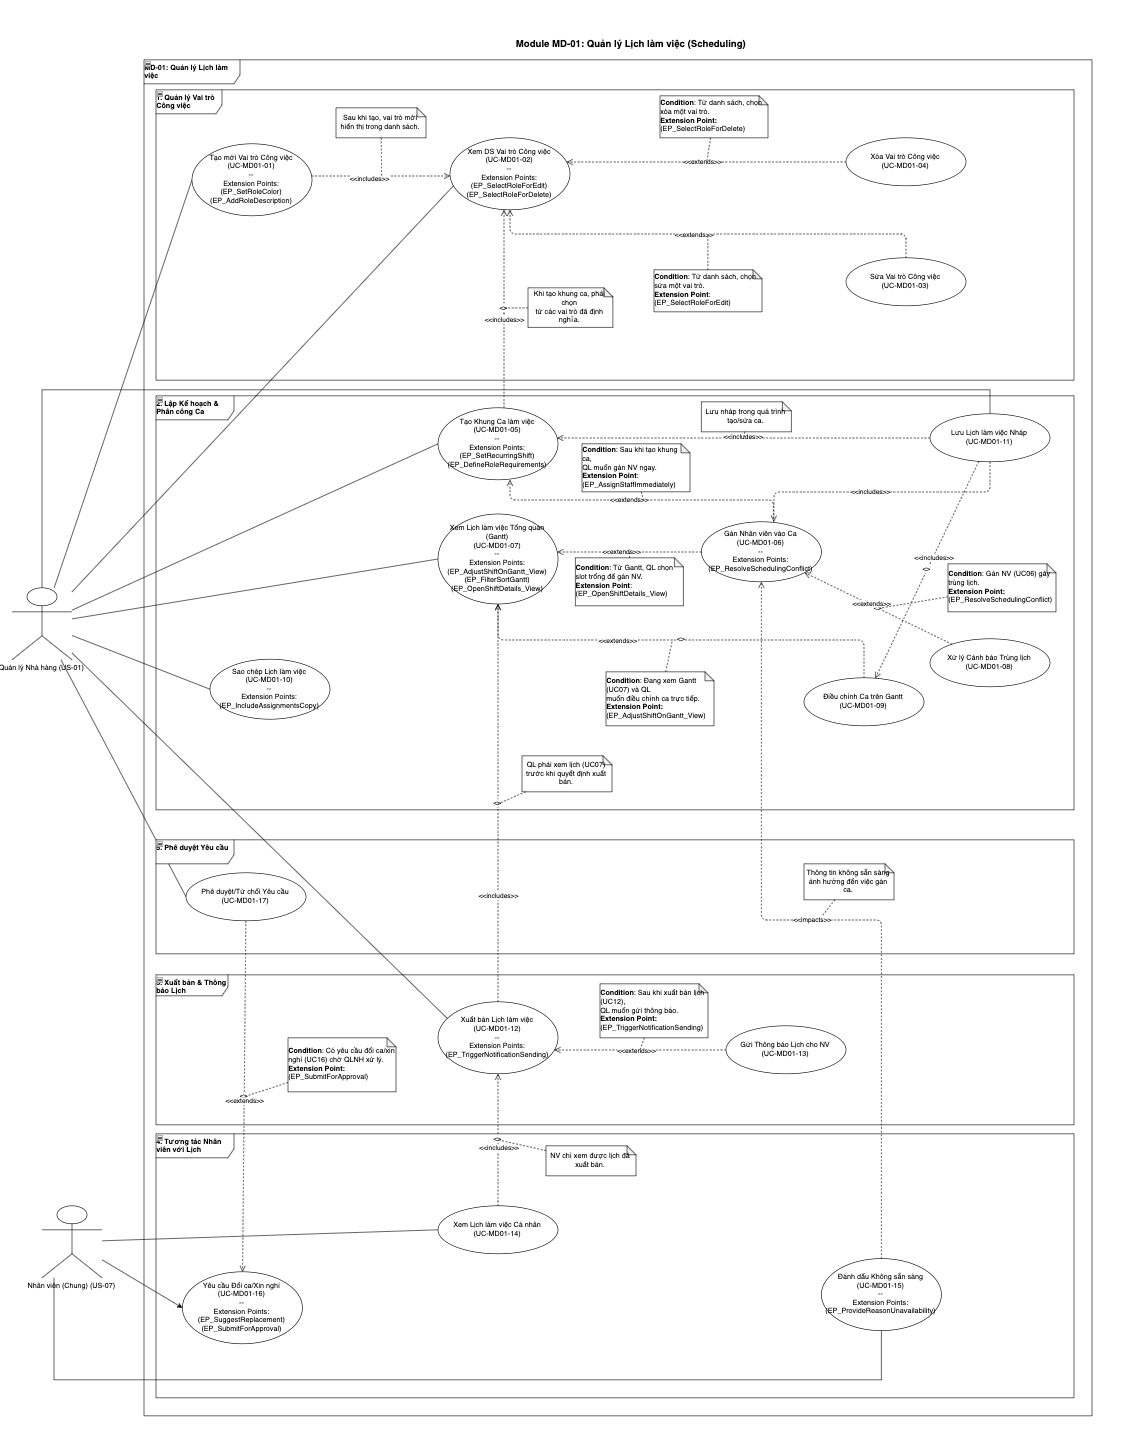
\includegraphics[width=15cm]{Sections/tong_quan/functional_spec/img/uc1.png}
    \vspace{0.5cm}
    \caption{Use case diagram cho Module MD-01}
    \label{fig:my_label}
\end{figure}

\begin{longtable}{|m{2cm}|m{2.5cm}|m{2cm}|m{4cm}|m{4.5cm}|}
    \caption{Danh sách Yêu cầu Chức năng cho Module MD-01: Quản lý Lịch làm việc} \label{tab:fr_md01_revised} \\
    \hline
    \textbf{Mã Module} & \textbf{Mã Yêu cầu CN} & \textbf{Mã Người dùng} & \textbf{Tên Chức năng} & \textbf{Mô tả Ngắn} \\
    \hline
    \endhead
    
    \hline
    \endfoot
    
    \hline
    \endlastfoot
    
    MD-01 & FR-MD01-01 & US-01 & Tạo mới Vai trò Công việc & Cho phép Quản lý nhà hàng định nghĩa một vai trò công việc mới (ví dụ: Bếp trưởng, Phục vụ). \\
    \hline
    MD-01 & FR-MD01-02 & US-01 & Xem Danh sách Vai trò Công việc & Cho phép Quản lý nhà hàng xem danh sách các vai trò công việc đã được định nghĩa. \\
    \hline
    MD-01 & FR-MD01-03 & US-01 & Sửa Thông tin Vai trò Công việc & Cho phép Quản lý nhà hàng chỉnh sửa thông tin của một vai trò công việc hiện có. \\
    \hline
    MD-01 & FR-MD01-04 & US-01 & Xóa Vai trò Công việc & Cho phép Quản lý nhà hàng xóa một vai trò công việc không còn sử dụng (nếu thỏa điều kiện). \\
    \hline
    MD-01 & FR-MD01-05 & US-01 & Tạo Khung Ca làm việc & Cho phép Quản lý nhà hàng định nghĩa các khung ca làm việc (thời gian, ngày, yêu cầu vai trò, số lượng). \\
    \hline
    MD-01 & FR-MD01-06 & US-01 & Gán Nhân viên vào Ca làm việc & Cho phép Quản lý nhà hàng chỉ định nhân viên cụ thể cho các vị trí trong khung ca đã tạo. \\
    \hline
    MD-01 & FR-MD01-07 & US-01 & Xem Lịch làm việc Tổng quan (Gantt) & Hiển thị lịch làm việc của tất cả nhân viên hoặc lọc theo vai trò dưới dạng biểu đồ Gantt. \\
    \hline
    MD-01 & FR-MD01-08 & US-01 & Xử lý Cảnh báo Trùng lịch & Khi hệ thống phát hiện trùng lịch (tự động), cho phép Quản lý nhà hàng xem xét và điều chỉnh việc gán ca để giải quyết xung đột. \\
    \hline
    MD-01 & FR-MD01-09 & US-01 & Điều chỉnh Ca làm việc trên Gantt & Cho phép Quản lý nhà hàng kéo thả, thay đổi kích thước, hoặc sửa đổi trực tiếp các ca trên biểu đồ Gantt. \\
    \hline
    MD-01 & FR-MD01-10 & US-01 & Sao chép Lịch làm việc (Ngày/Tuần/Tùy chỉnh) & Cho phép Quản lý nhà hàng sao chép nhanh lịch của một ngày, một tuần, hoặc một khoảng thời gian tùy chọn sang một thời điểm khác. \\
    \hline
    MD-01 & FR-MD01-11 & US-01 & Lưu Lịch làm việc Nháp & Cho phép Quản lý nhà hàng lưu lại các thay đổi trong lịch trình dưới dạng bản nháp. \\
    \hline
    MD-01 & FR-MD01-12 & US-01 & Xuất bản Lịch làm việc & Cho phép Quản lý nhà hàng công khai (publish) lịch làm việc đã được hoàn thiện. \\
    \hline
    MD-01 & FR-MD01-13 & US-01 & Gửi Thông báo Lịch làm việc cho Nhân viên & Kích hoạt hệ thống gửi thông báo (email/app) đến từng nhân viên về lịch trình cá nhân của họ sau khi lịch được xuất bản. \\
    \hline
    MD-01 & FR-MD01-14 & US-07 & Xem Lịch làm việc Cá nhân & Cho phép Nhân viên xem lịch làm việc đã được xuất bản của riêng mình. \\
    \hline
    MD-01 & FR-MD01-15 & US-07 & Đánh dấu Khoảng thời gian Không sẵn sàng & Cho phép Nhân viên (nếu được cấu hình) thông báo các khoảng thời gian không thể làm việc. \\
    \hline
    MD-01 & FR-MD01-16 & US-07 & Yêu cầu Đổi ca/Xin nghỉ & Cho phép Nhân viên (nếu được cấu hình) gửi yêu cầu đổi ca hoặc xin nghỉ thông qua hệ thống. \\
    \hline
    MD-01 & FR-MD01-17 & US-01 & Phê duyệt/Từ chối Yêu cầu Đổi ca/Xin nghỉ & Cho phép Quản lý nhà hàng xem xét và quyết định các yêu cầu đổi ca/xin nghỉ từ nhân viên. \\
    \hline
    
    \end{longtable}

\subsubsubsection{Mục tiêu và Phạm vi}
\label{sssec:md01_objectives_scope}
Mục tiêu chính của module MD-01 là:
\begin{itemize}
    \item \textbf{Tối ưu hóa việc sử dụng nhân lực:} Đảm bảo đủ nhân sự cho từng ca làm việc dựa trên nhu cầu hoạt động của nhà hàng, tránh tình trạng thiếu hoặc thừa nhân viên.
    \item \textbf{Minh bạch hóa lịch trình:} Cung cấp một cái nhìn tổng quan và chi tiết về lịch làm việc cho cả quản lý và nhân viên, giúp mọi người nắm rõ kế hoạch.
    \item \textbf{Giảm thiểu xung đột lịch trình:} Phát hiện và hỗ trợ giải quyết các trường hợp trùng lịch của nhân viên.
    \item \textbf{Tăng cường hiệu quả quản lý:} Tiết kiệm thời gian và công sức cho Quản lý nhà hàng trong việc lập lịch thủ công.
    \item \textbf{Cải thiện giao tiếp:} Tự động hóa việc thông báo lịch trình mới hoặc thay đổi cho nhân viên.
\end{itemize}
Phạm vi của module bao gồm toàn bộ quy trình quản lý lịch làm việc, từ khâu thiết lập ban đầu (vai trò công việc) đến khi lịch được công bố và nhân viên có thể tương tác (xem lịch, yêu cầu thay đổi).

\subsubsubsection{Đối tượng Sử dụng Chính}
\label{sssec:md01_primary_users}
Module này chủ yếu phục vụ hai nhóm đối tượng người dùng:
\begin{itemize}
    \item \textbf{US-01 (Quản lý nhà hàng):} Là người dùng chính, chịu trách nhiệm thực hiện hầu hết các chức năng của module như tạo vai trò, tạo khung ca, gán nhân viên, điều chỉnh lịch, xuất bản lịch, và phê duyệt các yêu cầu từ nhân viên.
    \item \textbf{US-07 (Nhân viên):} Là người dùng cuối, có thể xem lịch làm việc cá nhân đã được xuất bản, đánh dấu khoảng thời gian không sẵn sàng, và (tùy chọn) gửi yêu cầu đổi ca hoặc xin nghỉ.
\end{itemize}

\subsubsubsection{Các Chức năng Chính}
\label{sssec:md01_key_functionalities}
Module MD-01 cung cấp một bộ các chức năng toàn diện, được mô tả chi tiết qua các Use Case sau:

\begin{itemize}
    \item \textbf{Quản lý Vai trò Công việc (UC-MD01-01 đến UC-MD01-04):}
    \begin{itemize}
        \item Cho phép định nghĩa các vai trò công việc mới (ví dụ: "Đầu bếp chính", "Phục vụ bàn").
        \item Xem danh sách, sửa thông tin, và xóa các vai trò không còn sử dụng (với điều kiện ràng buộc).
    \end{itemize}

    \item \textbf{Lập Kế hoạch và Phân công Ca làm việc (UC-MD01-05, UC-MD01-06, UC-MD01-10, UC-MD01-11):}
    \begin{itemize}
        \item Tạo các khung ca làm việc, xác định thời gian và nhu cầu nhân sự (số lượng, vai trò) cho từng ca.
        \item Gán nhân viên cụ thể vào các vị trí còn trống trong khung ca, dựa trên sự phù hợp về vai trò và tính khả dụng.
        \item Sao chép lịch làm việc từ một ngày/tuần đã có sang ngày/tuần mới để tiết kiệm thời gian.
        \item Lưu trữ các thay đổi dưới dạng lịch nháp trước khi công bố.
    \end{itemize}

    \item \textbf{Trực quan hóa và Điều chỉnh Lịch (UC-MD01-07, UC-MD01-08, UC-MD01-09):}
    \begin{itemize}
        \item Hiển thị lịch làm việc tổng quan dưới dạng biểu đồ Gantt, cho phép lọc và nhóm theo nhân viên hoặc vai trò, thay đổi khung thời gian xem.
        \item Tự động phát hiện và cảnh báo các trường hợp trùng lịch của nhân viên, hỗ trợ Quản lý xử lý.
        \item Cho phép điều chỉnh nhanh ca làm việc (thay đổi thời gian, di chuyển ca, gán lại nhân viên) trực tiếp trên biểu đồ Gantt.
    \end{itemize}

    \item \textbf{Xuất bản và Thông báo Lịch (UC-MD01-12, UC-MD01-13):}
    \begin{itemize}
        \item Chính thức hóa lịch làm việc đã được xếp (chuyển từ "Nháp" sang "Đã xuất bản").
        \item Tự động gửi thông báo lịch làm việc cá nhân đến từng nhân viên sau khi lịch được xuất bản.
    \end{itemize}

    \item \textbf{Tương tác của Nhân viên (UC-MD01-14, UC-MD01-15, UC-MD01-16):}
    \begin{itemize}
        \item Cho phép nhân viên xem lịch làm việc cá nhân đã được xuất bản.
        \item Cho phép nhân viên chủ động đánh dấu các khoảng thời gian họ không thể làm việc.
        \item (Tùy chọn) Cho phép nhân viên gửi yêu cầu đổi ca hoặc xin nghỉ cho các ca đã được phân công.
    \end{itemize}

    \item \textbf{Quản lý Yêu cầu Nhân viên (UC-MD01-17):}
    \begin{itemize}
        \item (Tùy chọn) Cho phép Quản lý nhà hàng xem xét và phê duyệt hoặc từ chối các yêu cầu đổi ca/xin nghỉ từ nhân viên.
    \end{itemize}
\end{itemize}

\subsubsubsection{Tóm tắt Luồng Hoạt động Tổng thể}
\label{sssec:md01_overall_workflow}
Luồng hoạt động chính trong module MD-01 thường diễn ra như sau:
\begin{enumerate}
    \item \textbf{Thiết lập ban đầu:} Quản lý nhà hàng định nghĩa các Vai trò Công việc cần thiết (UC-MD01-01).
    \item \textbf{Tạo khung ca:} Quản lý tạo các Khung Ca làm việc cho một khoảng thời gian (ví dụ: tuần), xác định nhu cầu về số lượng và vai trò cho mỗi ca (UC-MD01-05). Có thể sử dụng chức năng Sao chép lịch để tăng tốc (UC-MD01-10).
    \item \textbf{Phân công nhân viên:} Quản lý gán từng Nhân viên cụ thể vào các vị trí trong khung ca (UC-MD01-06). Hệ thống hỗ trợ bằng cách gợi ý nhân viên phù hợp và cảnh báo nếu có thông tin không sẵn sàng (UC-MD01-15).
    \item \textbf{Rà soát và điều chỉnh:} Quản lý xem Lịch làm việc Tổng quan trên Gantt (UC-MD01-07), phát hiện và Xử lý Cảnh báo Trùng lịch (UC-MD01-08), và thực hiện các Điều chỉnh Ca cần thiết (UC-MD01-09). Mọi thay đổi được Lưu Nháp (UC-MD01-11).
    \item \textbf{Xuất bản và thông báo:} Sau khi hoàn tất, Quản lý Xuất bản Lịch làm việc (UC-MD01-12), và hệ thống Gửi Thông báo cho Nhân viên (UC-MD01-13).
    \item \textbf{Nhân viên tương tác:} Nhân viên Xem Lịch làm việc Cá nhân (UC-MD01-14). Nếu được phép, họ có thể Yêu cầu Đổi ca/Xin nghỉ (UC-MD01-16).
    \item \textbf{Xử lý yêu cầu:} Quản lý Phê duyệt/Từ chối các yêu cầu từ nhân viên (UC-MD01-17), và cập nhật lại lịch nếu cần.
\end{enumerate}
Module MD-01 đóng vai trò trung tâm trong việc đảm bảo hoạt động trơn tru hàng ngày của nhà hàng bằng cách quản lý hiệu quả nguồn lực quan trọng nhất: con người.

\subsubsection{Module MD-02: Quản lý Thực đơn \& Sản phẩm}
Module Quản lý Thực đơn \& Sản phẩm (MD-02) là một thành phần trung tâm trong hệ thống quản lý nhà hàng, đóng vai trò quan trọng trong việc định nghĩa, tổ chức và quản lý tất cả các mặt hàng mà nhà hàng cung cấp, từ món ăn, đồ uống đến các dịch vụ đi kèm. Module này cho phép Quản lý nhà hàng duy trì một cơ sở dữ liệu sản phẩm chính xác và chi tiết, làm nền tảng cho các hoạt động bán hàng, quản lý tồn kho (nếu có), và hiển thị trên giao diện Point of Sale (POS).


\begin{figure}[H]
    \centering
    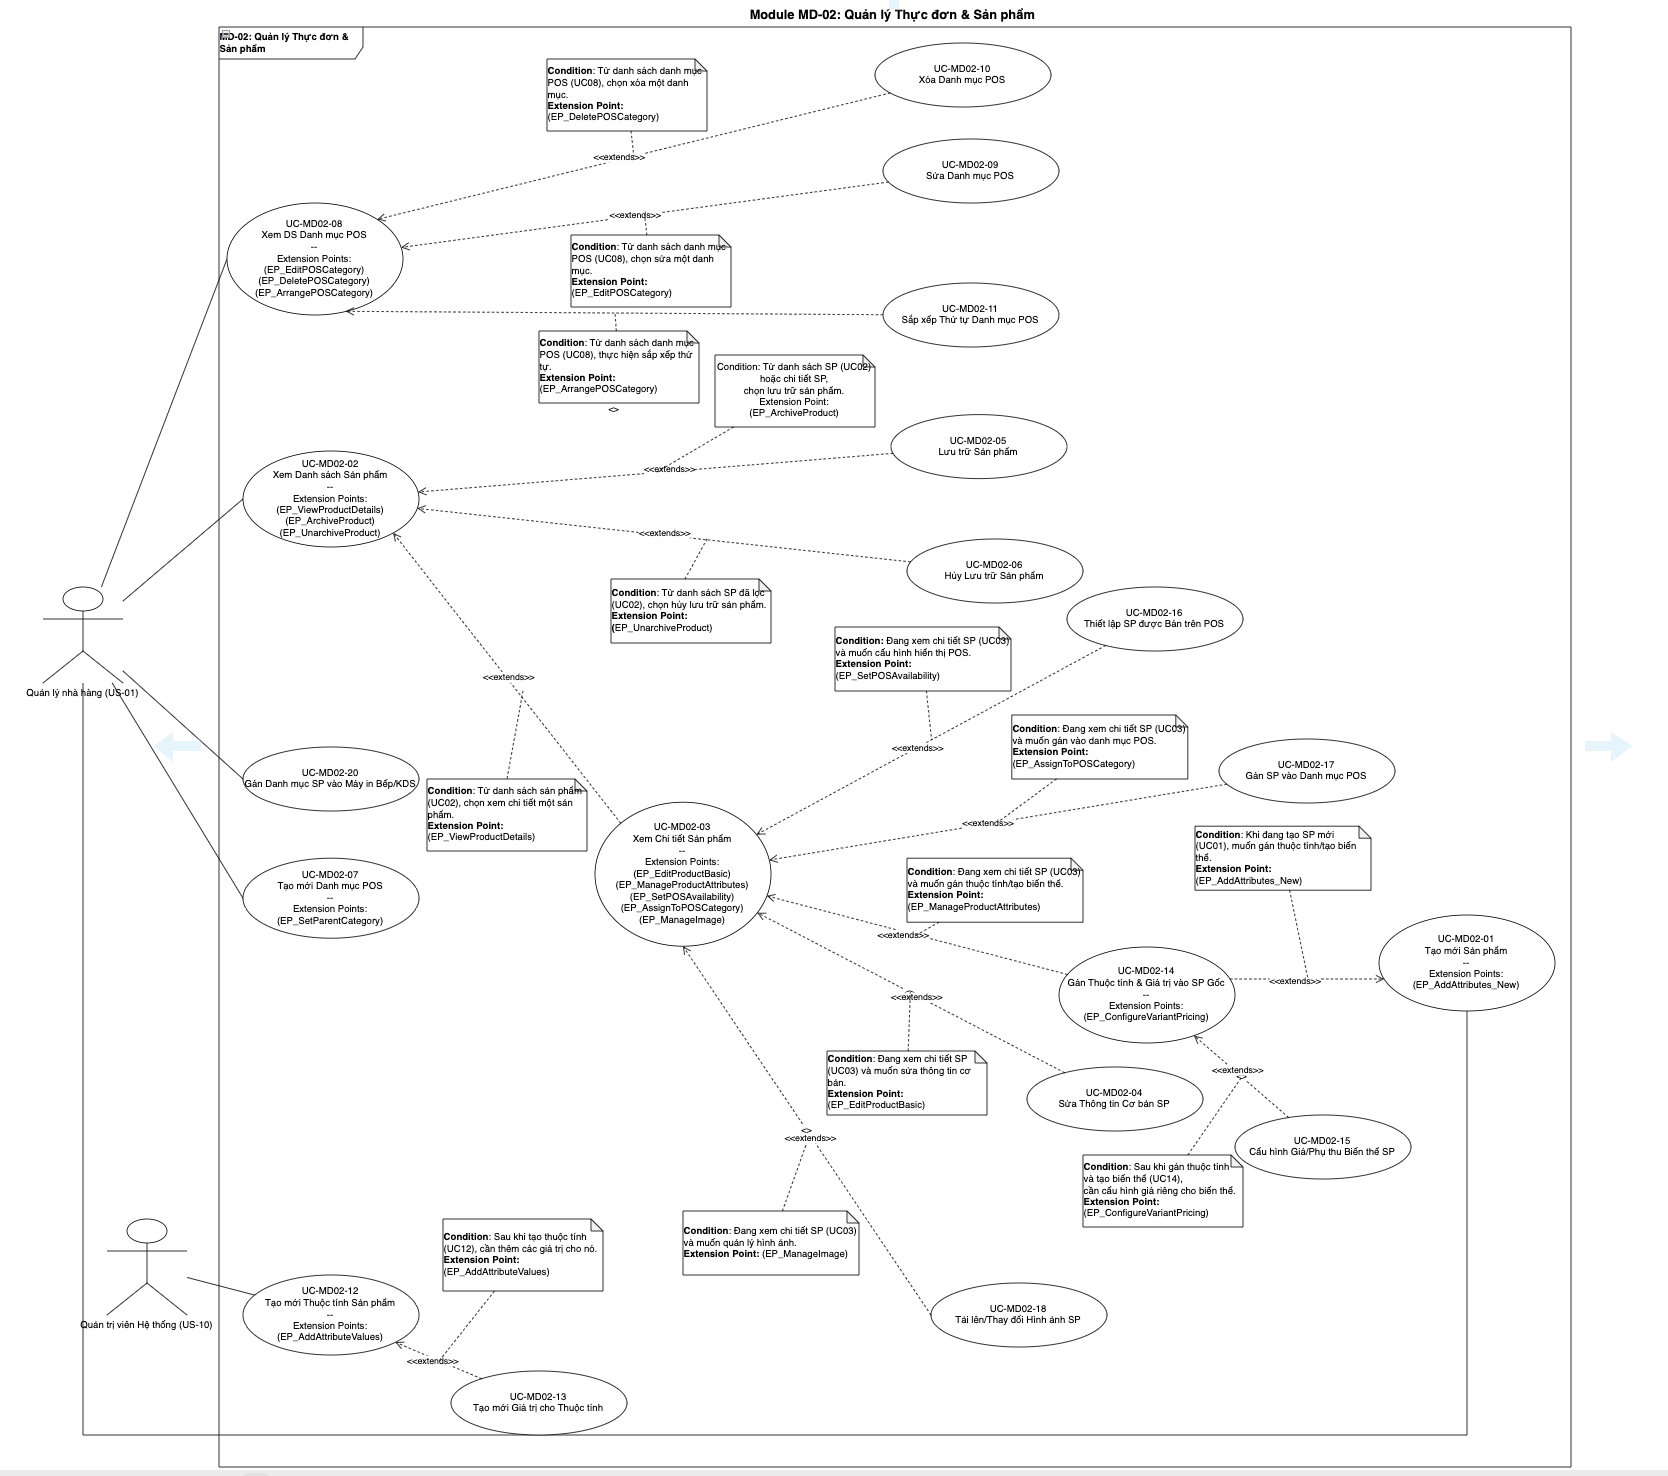
\includegraphics[width=15cm]{Sections/tong_quan/functional_spec/img/uc2.png}
    \vspace{0.5cm}
    \caption{Use case diagram cho Module MD-02}
    \label{fig:my_label}
\end{figure}

\begin{longtable}{|m{2cm}|m{2.5cm}|m{2cm}|m{4.5cm}|m{4cm}|}
\caption{Danh sách Yêu cầu Chức năng cho Module MD-02: Quản lý Thực đơn \& Sản phẩm} \label{tab:fr_md02_revised} \\
\hline
\textbf{Mã Module} & \textbf{Mã Yêu cầu CN} & \textbf{Mã Người dùng} & \textbf{Tên Chức năng} & \textbf{Mô tả Ngắn} \\
\hline
\endhead % Header cho các trang tiếp theo

\hline
\endfoot % Footer cho bảng

\hline
\endlastfoot % Footer cho trang cuối cùng

MD-02 & FR-MD02-01 & US-01 & Tạo mới Sản phẩm & Cho phép Quản lý nhà hàng thêm một món ăn, đồ uống, hoặc dịch vụ mới vào hệ thống (Tên, Giá, Loại...). \\
\hline
MD-02 & FR-MD02-02 & US-01 & Xem Danh sách Sản phẩm & Cho phép Quản lý nhà hàng xem danh sách tất cả các sản phẩm hiện có trong hệ thống. \\
\hline
MD-02 & FR-MD02-03 & US-01 & Xem Chi tiết Sản phẩm & Cho phép Quản lý nhà hàng xem thông tin chi tiết đầy đủ của một sản phẩm cụ thể. \\
\hline
MD-02 & FR-MD02-04 & US-01 & Sửa Thông tin Cơ bản của Sản phẩm & Cho phép Quản lý nhà hàng cập nhật các thông tin chung của sản phẩm (Tên, Loại, Giá bán, Giá vốn, Mã nội bộ...). \\
\hline
MD-02 & FR-MD02-05 & US-01 & Lưu trữ Sản phẩm & Cho phép Quản lý nhà hàng ẩn một sản phẩm khỏi các giao dịch mà không xóa hẳn dữ liệu (Archive). \\
\hline
MD-02 & FR-MD02-06 & US-01 & Hủy Lưu trữ Sản phẩm & Cho phép Quản lý nhà hàng kích hoạt lại một sản phẩm đã bị lưu trữ để bán/sử dụng lại (Unarchive). \\
\hline
MD-02 & FR-MD02-07 & US-01 & Tạo mới Danh mục POS & Cho phép Quản lý nhà hàng tạo một danh mục mới để nhóm sản phẩm trên giao diện POS. \\
\hline
MD-02 & FR-MD02-08 & US-01 & Xem Danh sách Danh mục POS & Cho phép Quản lý nhà hàng xem danh sách các danh mục POS đã tạo. \\
\hline
MD-02 & FR-MD02-09 & US-01 & Sửa Danh mục POS & Cho phép Quản lý nhà hàng chỉnh sửa thông tin (Tên, Thứ tự, Cha...) của một danh mục POS. \\
\hline
MD-02 & FR-MD02-10 & US-01 & Xóa Danh mục POS & Cho phép Quản lý nhà hàng xóa một danh mục POS (nếu thỏa điều kiện). \\
\hline
MD-02 & FR-MD02-11 & US-01 & Sắp xếp Thứ tự Danh mục POS & Cho phép Quản lý nhà hàng thay đổi thứ tự hiển thị của các danh mục POS. \\
\hline
MD-02 & FR-MD02-12 & US-01/US-10 & Tạo mới Thuộc tính Sản phẩm & Cho phép định nghĩa một đặc tính mới cho sản phẩm (ví dụ: Kích cỡ, Màu sắc). \\
\hline
MD-02 & FR-MD02-13 & US-01/US-10 & Tạo mới Giá trị cho Thuộc tính & Cho phép định nghĩa các lựa chọn cụ thể cho một thuộc tính (ví dụ: S, M, L cho Kích cỡ). \\
\hline
MD-02 & FR-MD02-14 & US-01 & Gán Thuộc tính và Giá trị vào Sản phẩm Gốc & Cho phép Quản lý nhà hàng áp dụng các thuộc tính và giá trị đã định nghĩa vào một sản phẩm gốc. \\
\hline
MD-02 & FR-MD02-15 & US-01 & Cấu hình Giá/Phụ thu cho Biến thể Sản phẩm & Cho phép Quản lý nhà hàng đặt giá bán khác nhau hoặc giá trị phụ thu cho từng biến thể sản phẩm cụ thể. \\
\hline
MD-02 & FR-MD02-16 & US-01 & Thiết lập Sản phẩm được Bán trên POS & Cho phép Quản lý nhà hàng đánh dấu một sản phẩm là có sẵn để bán trên POS. \\
\hline
MD-02 & FR-MD02-17 & US-01 & Gán Sản phẩm vào Danh mục POS & Cho phép Quản lý nhà hàng chỉ định một sản phẩm thuộc về (các) danh mục nào trên POS. \\
\hline
MD-02 & FR-MD02-18 & US-01 & Tải lên/Thay đổi Hình ảnh Sản phẩm & Cho phép Quản lý nhà hàng quản lý hình ảnh đại diện cho sản phẩm. \\
\hline
MD-02 & FR-MD02-19 & US-01 & Xóa Hình ảnh Sản phẩm & Cho phép Quản lý nhà hàng xóa hình ảnh hiện tại của sản phẩm. \\
\hline
MD-02 & FR-MD02-20 & US-01 & Gán Danh mục Sản phẩm vào Máy in Bếp/KDS & Cho phép Quản lý nhà hàng chỉ định danh mục sản phẩm nào sẽ gửi đến thiết bị bếp/KDS nào (Cấu hình này thường nằm trong Cài đặt POS). \\
\hline

\end{longtable}

\subsubsubsection{Mục tiêu và Phạm vi}
\label{sssec:md02_objectives_scope}
Mục tiêu chính của module MD-02 là:
\begin{itemize}
    \item \textbf{Quản lý tập trung danh mục sản phẩm:} Cung cấp một nơi duy nhất để tạo, sửa, xóa và xem thông tin chi tiết của tất cả các món ăn, đồ uống, và dịch vụ.
    \item \textbf{Hỗ trợ định giá linh hoạt:} Cho phép thiết lập giá bán, giá vốn, và quản lý giá cho các biến thể sản phẩm khác nhau.
    \item \textbf{Tổ chức thực đơn cho POS:} Cho phép tạo và quản lý các danh mục sản phẩm để hiển thị một cách khoa học và dễ sử dụng trên màn hình Point of Sale.
    \item \textbf{Quản lý biến thể sản phẩm:} Hỗ trợ tạo và quản lý các phiên bản khác nhau của cùng một sản phẩm (ví dụ: kích cỡ, độ cay, topping) với các mức giá tương ứng.
    \item \textbf{Tích hợp với các module khác:} Đảm bảo dữ liệu sản phẩm được sử dụng nhất quán trong các module Bán hàng, Kho (Inventory), Kế toán, và Point of Sale.
    \item \textbf{Cấu hình hiển thị và in ấn:} Cho phép tùy chỉnh hình ảnh sản phẩm và cấu hình cách các đơn hàng được gửi đến máy in bếp hoặc Màn hình Hiển thị Bếp (KDS).
\end{itemize}
Phạm vi của module bao gồm toàn bộ vòng đời của một sản phẩm trong hệ thống, từ việc tạo mới, cấu hình chi tiết, quản lý các thuộc tính và biến thể, tổ chức hiển thị trên POS, cho đến việc lưu trữ hoặc ngừng kinh doanh sản phẩm.

\subsubsubsection{Đối tượng Sử dụng Chính}
\label{sssec:md02_primary_users}
Module này chủ yếu được sử dụng bởi:
\begin{itemize}
    \item \textbf{US-01 (Quản lý nhà hàng):} Là người dùng chính, chịu trách nhiệm thực hiện hầu hết các chức năng của module như tạo mới sản phẩm, cập nhật giá, quản lý danh mục POS, cấu hình biến thể, và thiết lập hiển thị trên POS.
    \item \textbf{US-10 (Quản trị viên Hệ thống):} Có thể tham gia vào việc tạo và quản lý các Thuộc tính sản phẩm dùng chung hoặc các cấu hình hệ thống liên quan đến sản phẩm.
\end{itemize}
Nhân viên bán hàng (US-03) sẽ tương tác gián tiếp với module này thông qua giao diện POS, nơi họ chọn các sản phẩm đã được cấu hình.

\subsubsubsection{Các Chức năng Chính}
\label{sssec:md02_key_functionalities}
Module MD-02 cung cấp một loạt các chức năng thiết yếu, được mô tả chi tiết qua các Use Case sau:

\begin{itemize}
    \item \textbf{Quản lý Thông tin Sản phẩm Cơ bản (UC-MD02-01 đến UC-MD02-06, UC-MD02-18, UC-MD02-19):}
    \begin{itemize}
        \item Tạo mới một sản phẩm (món ăn, đồ uống, dịch vụ) với các thông tin ban đầu như tên, loại, giá bán, giá vốn (UC-MD02-01).
        \item Xem danh sách toàn bộ sản phẩm với các tùy chọn tìm kiếm, lọc và nhóm (UC-MD02-02).
        \item Xem thông tin chi tiết đầy đủ của một sản phẩm cụ thể (UC-MD02-03).
        \item Sửa đổi các thông tin cơ bản của sản phẩm đã tồn tại (UC-MD02-04).
        \item Lưu trữ (ẩn đi) các sản phẩm không còn kinh doanh và hủy lưu trữ khi cần (UC-MD02-05, UC-MD02-06).
        \item Tải lên, thay đổi hoặc xóa hình ảnh đại diện cho sản phẩm (UC-MD02-18, UC-MD02-19).
    \end{itemize}

    \item \textbf{Quản lý Danh mục Point of Sale (POS) (UC-MD02-07 đến UC-MD02-11):}
    \begin{itemize}
        \item Tạo mới các danh mục để phân loại sản phẩm trên giao diện POS (ví dụ: "Khai vị", "Món chính") (UC-MD02-07).
        \item Xem, sửa, xóa và sắp xếp thứ tự hiển thị của các danh mục POS (UC-MD02-08, UC-MD02-09, UC-MD02-10, UC-MD02-11).
    \end{itemize}

    \item \textbf{Quản lý Thuộc tính và Biến thể Sản phẩm (UC-MD02-12 đến UC-MD02-15):}
    \begin{itemize}
        \item Tạo mới các thuộc tính chung cho sản phẩm (ví dụ: "Kích cỡ", "Màu sắc", "Độ cay") (UC-MD02-12).
        \item Định nghĩa các giá trị cụ thể cho từng thuộc tính (ví dụ: "Nhỏ", "Vừa", "Lớn" cho thuộc tính "Kích cỡ") (UC-MD02-13).
        \item Gán các thuộc tính và giá trị đã chọn vào một sản phẩm gốc, từ đó tự động tạo ra các sản phẩm biến thể (UC-MD02-14).
        \item Cấu hình giá bán riêng hoặc mức phụ thu cho từng biến thể sản phẩm cụ thể (UC-MD02-15).
    \end{itemize}

    \item \textbf{Cấu hình Sản phẩm cho Point of Sale (UC-MD02-16, UC-MD02-17, UC-MD02-20):}
    \begin{itemize}
        \item Thiết lập cho phép hoặc không cho phép một sản phẩm được bán trên giao diện POS (UC-MD02-16).
        \item Gán một sản phẩm vào một hoặc nhiều danh mục POS để hiển thị đúng nhóm trên menu (UC-MD02-17).
        \item Cấu hình việc định tuyến các danh mục sản phẩm đến các máy in bếp hoặc màn hình KDS cụ thể khi có đơn hàng (UC-MD02-20).
    \end{itemize}
\end{itemize}

\subsubsubsection{Tóm tắt Luồng Hoạt động Tổng thể}
\label{sssec:md02_overall_workflow}
Luồng hoạt động điển hình trong module Quản lý Thực đơn \& Sản phẩm bao gồm các bước chính sau:
\begin{enumerate}
    \item \textbf{Tạo sản phẩm mới:} Quản lý nhà hàng Tạo mới Sản phẩm với các thông tin cơ bản như tên, giá, loại (UC-MD02-01).
    \item \textbf{Cấu hình chi tiết sản phẩm:}
        \begin{itemize}
            \item Tải lên Hình ảnh Sản phẩm (UC-MD02-18).
            \item Nếu sản phẩm có nhiều phiên bản, Quản lý sẽ Tạo mới Thuộc tính (UC-MD02-12), Tạo mới Giá trị cho Thuộc tính (UC-MD02-13), Gán Thuộc tính và Giá trị vào Sản phẩm Gốc để tạo biến thể (UC-MD02-14), và Cấu hình Giá/Phụ thu cho Biến thể (UC-MD02-15).
        \end{itemize}
    \item \textbf{Chuẩn bị cho POS:}
        \begin{itemize}
            \item Quản lý Tạo mới Danh mục POS nếu cần (UC-MD02-07) hoặc Sắp xếp Thứ tự Danh mục POS (UC-MD02-11).
            \item Thiết lập Sản phẩm được Bán trên POS (UC-MD02-16).
            \item Gán Sản phẩm vào Danh mục POS tương ứng (UC-MD02-17).
            \item Gán Danh mục Sản phẩm vào Máy in Bếp/KDS để định tuyến đơn hàng (UC-MD02-20).
        \end{itemize}
    \item \textbf{Bảo trì và cập nhật:}
        \begin{itemize}
            \item Quản lý thường xuyên Xem Danh sách Sản phẩm (UC-MD02-02) và Xem Chi tiết Sản phẩm (UC-MD02-03).
            \item Thực hiện Sửa Thông tin Cơ bản của Sản phẩm khi cần (ví dụ: thay đổi giá) (UC-MD02-04).
            \item Lưu trữ Sản phẩm không còn kinh doanh (UC-MD02-05) hoặc Hủy Lưu trữ Sản phẩm khi muốn bán lại (UC-MD02-06).
            \item Quản lý Danh mục POS: Sửa (UC-MD02-09) hoặc Xóa (UC-MD02-10) khi cần thiết.
        \end{itemize}
\end{enumerate}
Module MD-02 đảm bảo rằng thực đơn của nhà hàng luôn được cập nhật, chính xác và được trình bày một cách tối ưu trên các hệ thống bán hàng, góp phần vào trải nghiệm khách hàng tốt và hiệu quả vận hành.

\subsubsection{Module MD-03: Quản lý Đặt chỗ \& Đặt món trước}
Module Quản lý Đặt chỗ \& Đặt món trước (MD-03) được thiết kế để cung cấp một giải pháp toàn diện cho nhà hàng trong việc quản lý các yêu cầu đặt bàn từ khách hàng, cả qua kênh trực tuyến lẫn các kênh truyền thống. Module này không chỉ giúp tối ưu hóa việc sử dụng không gian và nguồn lực của nhà hàng mà còn nâng cao trải nghiệm của khách hàng bằng cách cho phép họ chủ động tìm kiếm, lựa chọn thời gian, bàn (tùy chọn), và thậm chí đặt trước các món ăn mong muốn.



\begin{figure}[H]
    \centering
    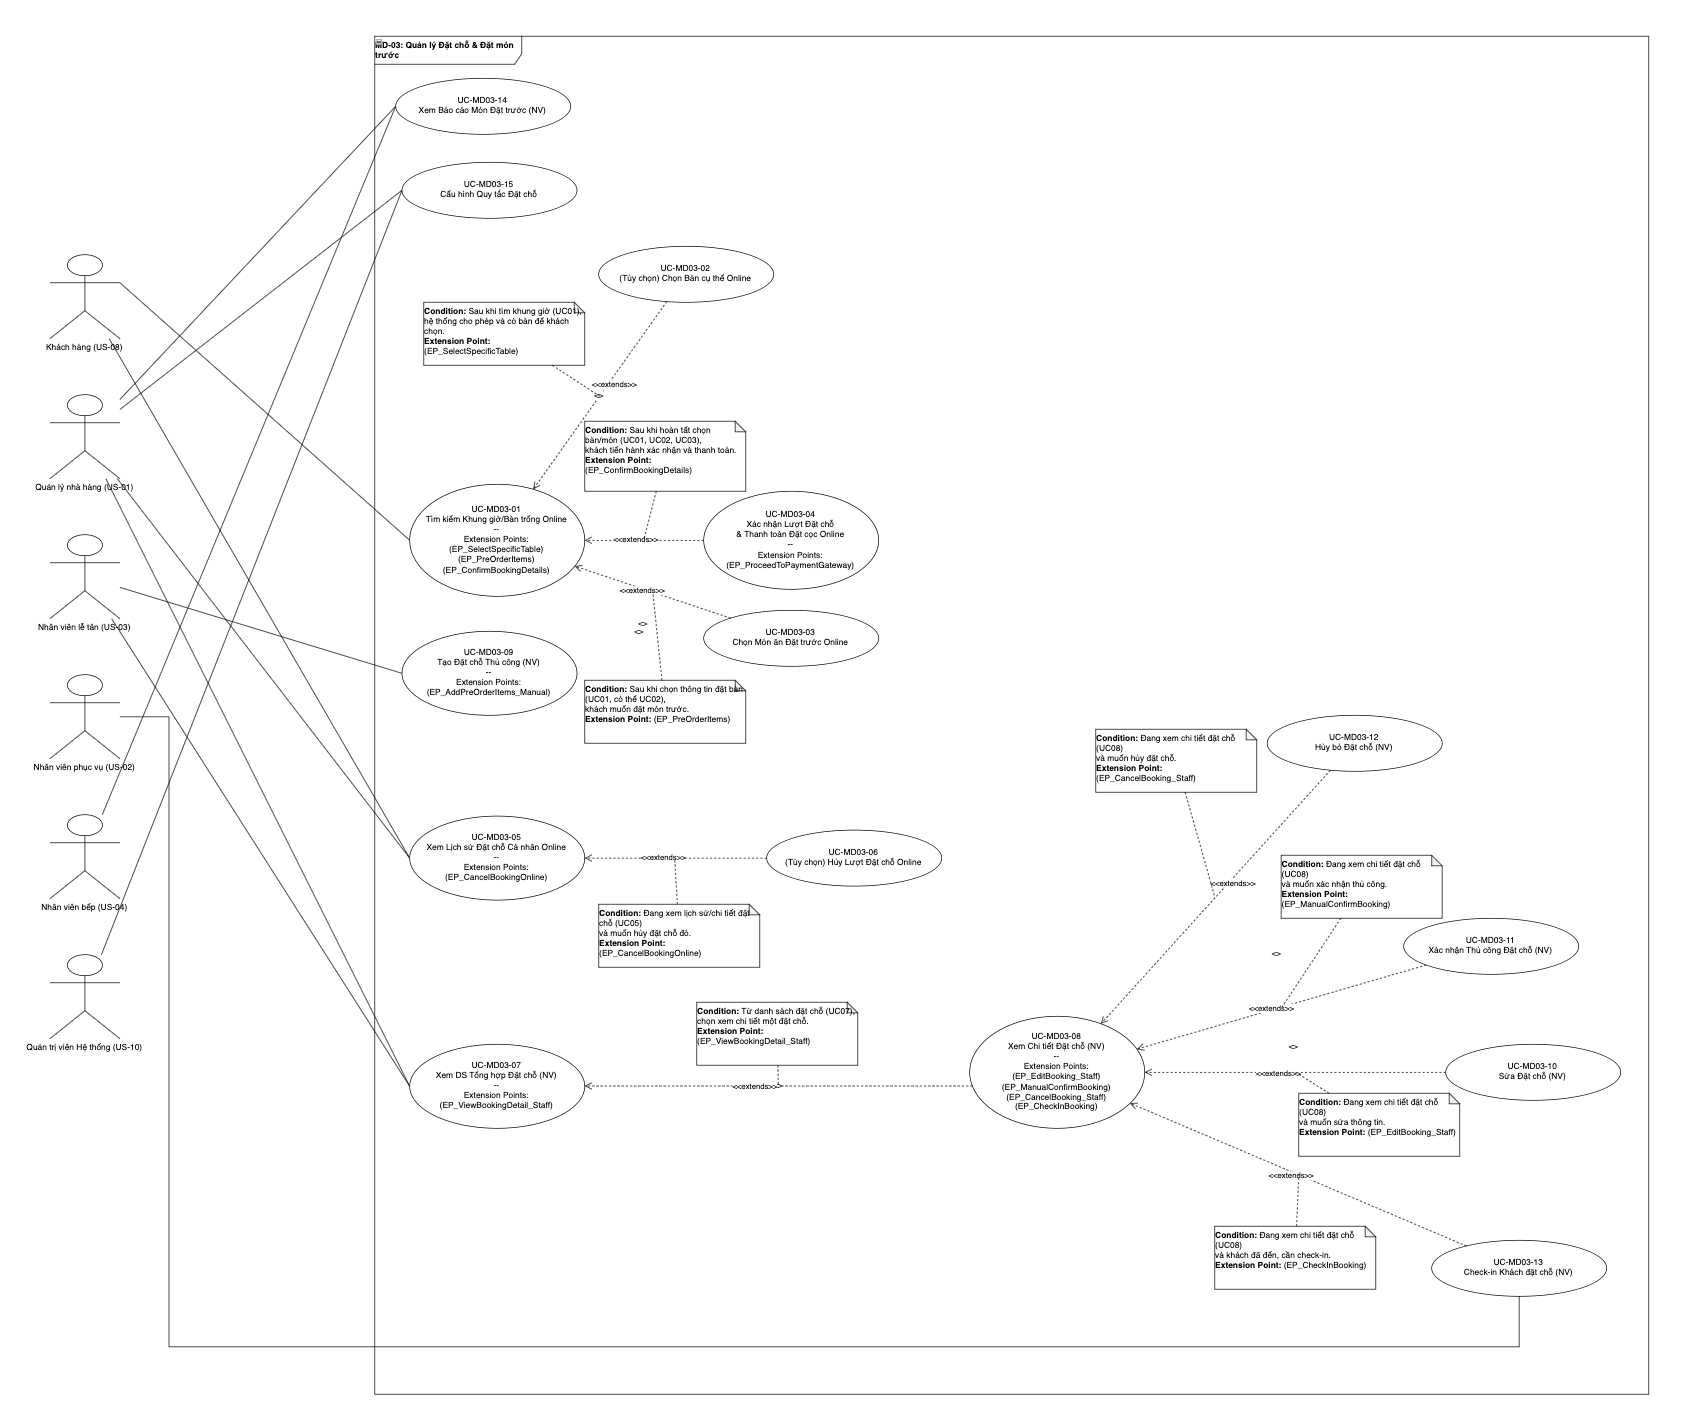
\includegraphics[width=15cm]{Sections/tong_quan/functional_spec/img/uc3.png}
    \vspace{0.5cm}
    \caption{Use case diagram cho Module MD-03}
    \label{fig:my_label}
\end{figure}

\begin{longtable}{|m{2cm}|m{2.5cm}|m{2cm}|m{4.5cm}|m{4cm}|}
\caption{Danh sách Yêu cầu Chức năng cho Module MD-03: Quản lý Đặt chỗ \& Đặt món trước} \label{tab:fr_md03_revised_v3} \\
\hline
\textbf{Mã Module} & \textbf{Mã Yêu cầu CN} & \textbf{Mã Người dùng} & \textbf{Tên Chức năng} & \textbf{Mô tả Ngắn} \\
\hline
\endhead % Header cho các trang tiếp theo
\hline
\endfoot % Footer cho bảng
\hline
\endlastfoot % Footer cho trang cuối cùng

% === Luồng Khách hàng Đặt Online ===
MD-03 & FR-MD03-01 & US-08 & Tìm kiếm Khung giờ/Bàn trống Online & Khách hàng nhập ngày, giờ, số người để tìm kiếm các lựa chọn đặt bàn còn trống. \\
\hline
MD-03 & FR-MD03-02 & US-08 & (Tùy chọn) Chọn Bàn cụ thể từ Sơ đồ tầng Online & Khách hàng xem sơ đồ và chọn bàn trống cụ thể (nếu được phép). \\
\hline
MD-03 & FR-MD03-03 & US-08 & Chọn Món ăn Đặt trước từ Thực đơn Online & Khách hàng duyệt thực đơn và thêm các món muốn đặt trước vào giỏ hàng. \\
\hline
MD-03 & FR-MD03-04 & US-08 & Xác nhận Lượt Đặt chỗ và Thanh toán Đặt cọc Online & Khách hàng xem lại toàn bộ thông tin, nhập thông tin cá nhân và thực hiện thanh toán tiền đặt cọc. \\
\hline
MD-03 & FR-MD03-05 & US-08 & Xem Lịch sử Đặt chỗ Cá nhân Online & Khách hàng đã đăng nhập xem lại các đặt chỗ đã thực hiện. \\
\hline
MD-03 & FR-MD03-06 & US-08 & (Tùy chọn) Hủy Lượt Đặt chỗ Online & Khách hàng hủy một đặt chỗ đã xác nhận (nếu còn trong thời hạn và chính sách cho phép). \\
\hline

% === Luồng Nhân viên Quản lý Đặt chỗ ===
MD-03 & FR-MD03-07 & US-01/US-03 & Xem Danh sách Tổng hợp các Lượt Đặt chỗ & Nhân viên xem danh sách tất cả các đặt chỗ với bộ lọc/tìm kiếm. \\
\hline
MD-03 & FR-MD03-08 & US-01/US-03 & Xem Thông tin Chi tiết một Lượt Đặt chỗ & Nhân viên xem đầy đủ chi tiết của một đặt chỗ cụ thể. \\
\hline
MD-03 & FR-MD03-09 & US-01/US-03 & Tạo mới Lượt Đặt chỗ Thủ công (Backend/POS) & Nhân viên nhập thông tin để tạo đặt chỗ cho khách qua điện thoại/trực tiếp. \\
\hline
MD-03 & FR-MD03-10 & US-01/US-03 & Sửa Thông tin Lượt Đặt chỗ (Backend/POS) & Nhân viên cập nhật các thông tin của một đặt chỗ đã có. \\
\hline
MD-03 & FR-MD03-11 & US-01/US-03 & Xác nhận Thủ công Lượt Đặt chỗ & Nhân viên chuyển trạng thái một đặt chỗ (ví dụ: từ chờ sang đã xác nhận). \\
\hline
MD-03 & FR-MD03-12 & US-01/US-03 & Hủy bỏ Lượt Đặt chỗ (Backend/POS) & Nhân viên hủy một đặt chỗ, có thể kèm lý do. \\
\hline
MD-03 & FR-MD03-13 & US-01/US-03 & Đánh dấu Khách đã đến (Check-in) cho Lượt Đặt chỗ & Nhân viên ghi nhận khách đã đến nhận bàn. \\
\hline
MD-03 & FR-MD03-14 & US-04/US-01 & Xem Báo cáo Tổng hợp Món ăn Cần chuẩn bị (Đặt trước) & Nhân viên bếp/quản lý xem các món đã được khách đặt trước. \\
\hline

% === Luồng Cấu hình ===
MD-03 & FR-MD03-15 & US-01/US-10 & Cấu hình Quy tắc và Tham số Đặt chỗ & Thiết lập giờ, giới hạn khách, quy tắc cọc, giá trị bàn, cho phép chọn bàn online... \\
\hline

\end{longtable}



\subsubsubsection{Mục tiêu và Phạm vi}
\label{sssec:md03_objectives_scope}
Mục tiêu chính của module MD-03 bao gồm:
\begin{itemize}
    \item \textbf{Tối ưu hóa quy trình đặt chỗ:} Tự động hóa việc tìm kiếm và xác nhận đặt bàn, giảm thiểu công việc thủ công cho nhân viên.
    \item \textbf{Nâng cao trải nghiệm khách hàng:} Cung cấp giao diện trực tuyến thân thiện cho khách hàng tự tìm kiếm, đặt bàn, chọn món và thanh toán đặt cọc.
    \item \textbf{Quản lý hiệu quả tình trạng bàn:} Cung cấp cái nhìn tổng quan về tình trạng đặt bàn, giúp nhân viên sắp xếp và quản lý khách hiệu quả hơn.
    \item \textbf{Giảm thiểu tình trạng no-show:} Thông qua việc yêu cầu đặt cọc (nếu có) và gửi thông báo nhắc nhở.
    \item \textbf{Hỗ trợ chuẩn bị cho bếp:} Nếu có chức năng đặt món trước, cung cấp thông tin sớm cho bộ phận bếp để chuẩn bị nguyên liệu và chế biến.
    \item \textbf{Linh hoạt trong cấu hình:} Cho phép nhà hàng tùy chỉnh các quy tắc đặt chỗ (giờ hoạt động, giới hạn khách, chính sách đặt cọc) cho phù hợp với mô hình kinh doanh.
\end{itemize}
Phạm vi của module bao gồm toàn bộ quy trình từ khi khách hàng bắt đầu tìm kiếm đặt chỗ online, chọn món (nếu có), thanh toán đặt cọc, nhận xác nhận, cho đến khi nhân viên nhà hàng quản lý các lượt đặt chỗ này, cập nhật trạng thái (check-in, hủy), và xem báo cáo liên quan.

\subsubsubsection{Đối tượng Sử dụng Chính}
\label{sssec:md03_primary_users}
Module này phục vụ các nhóm đối tượng người dùng sau:
\begin{itemize}
    \item \textbf{US-08 (Khách hàng):} Là người dùng chính của các chức năng đặt chỗ trực tuyến, bao gồm tìm kiếm bàn trống, chọn món, thanh toán đặt cọc và xem lại lịch sử đặt chỗ.
    \item \textbf{US-01 (Quản lý nhà hàng):} Chịu trách nhiệm cấu hình các quy tắc đặt chỗ, xem báo cáo, quản lý các lượt đặt chỗ có vấn đề, và có thể thực hiện tất cả các thao tác quản lý đặt chỗ.
    \item \textbf{US-03 (Nhân viên lễ tân):} Thường xuyên làm việc với module để xem danh sách đặt chỗ, tạo đặt chỗ thủ công, sửa thông tin, xác nhận, hủy, và đánh dấu khách đã đến.
    \item \textbf{US-04 (Nhân viên bếp):} (Nếu có đặt món trước) Xem báo cáo các món ăn cần chuẩn bị.
    \item \textbf{US-10 (Quản trị viên Hệ thống):} Có thể tham gia vào việc cấu hình các tham số hệ thống sâu hơn liên quan đến module đặt chỗ.
\end{itemize}

\subsubsubsection{Các Chức năng Chính}
\label{sssec:md03_key_functionalities}
Module MD-03 cung cấp một tập hợp các chức năng đa dạng, được mô tả chi tiết qua các Use Case sau:

\begin{itemize}
    \item \textbf{Đặt chỗ Trực tuyến từ Khách hàng (UC-MD03-01 đến UC-MD03-06):}
    \begin{itemize}
        \item Cho phép khách hàng tìm kiếm khung giờ và bàn trống dựa trên ngày, giờ và số lượng người (UC-MD03-01).
        \item (Tùy chọn) Cho phép khách hàng chọn một bàn cụ thể từ sơ đồ tầng online (UC-MD03-02).
        \item Cho phép khách hàng duyệt thực đơn và chọn các món ăn/đồ uống để đặt trước (UC-MD03-03).
        \item Khách hàng xem lại thông tin, cung cấp chi tiết liên hệ và thực hiện thanh toán đặt cọc (nếu có) để xác nhận đặt chỗ (UC-MD03-04).
        \item Cho phép khách hàng đã đăng nhập xem lại lịch sử các lượt đặt chỗ cá nhân (UC-MD03-05).
        \item (Tùy chọn) Cho phép khách hàng tự hủy một lượt đặt chỗ đã xác nhận, tuân theo chính sách của nhà hàng (UC-MD03-06).
    \end{itemize}

    \item \textbf{Quản lý Lượt Đặt chỗ bởi Nhân viên (UC-MD03-07 đến UC-MD03-13):}
    \begin{itemize}
        \item Cho phép nhân viên xem danh sách tổng hợp các lượt đặt chỗ với khả năng lọc và tìm kiếm (UC-MD03-07).
        \item Tạo mới một lượt đặt chỗ thủ công trong hệ thống (ví dụ: cho khách đặt qua điện thoại) (UC-MD03-09).
        \item Xem thông tin chi tiết đầy đủ của một lượt đặt chỗ cụ thể (UC-MD03-08).
        \item Sửa đổi các thông tin của một lượt đặt chỗ đã tồn tại (UC-MD03-10).
        \item Xác nhận thủ công một lượt đặt chỗ (ví dụ: chuyển từ "Chờ xác nhận" sang "Đã xác nhận") (UC-MD03-11).
        \item Hủy bỏ một lượt đặt chỗ trong hệ thống (UC-MD03-12).
        \item Đánh dấu khách hàng đã đến (check-in) cho một lượt đặt chỗ (UC-MD03-13).
    \end{itemize}

    \item \textbf{Báo cáo và Cấu hình (UC-MD03-14, UC-MD03-15):}
    \begin{itemize}
        \item Cung cấp báo cáo tổng hợp các món ăn cần chuẩn bị cho các lượt đặt chỗ có đặt món trước (UC-MD03-14).
        \item Cho phép Quản lý/Quản trị viên cấu hình các quy tắc và tham số vận hành cho chức năng đặt chỗ (UC-MD03-15).
    \end{itemize}
\end{itemize}

\subsubsubsection{Tóm tắt Luồng Hoạt động Tổng thể}
\label{sssec:md03_overall_workflow}
Luồng hoạt động chính trong module MD-03 có thể được tóm tắt như sau:

\begin{enumerate}
    \item \textbf{Cấu hình ban đầu:} Quản lý nhà hàng Cấu hình Quy tắc và Tham số Đặt chỗ (UC-MD03-15) như giờ hoạt động, chính sách đặt cọc, v.v.
    \item \textbf{Khách hàng đặt chỗ online:}
        \begin{itemize}
            \item Khách hàng Tìm kiếm Khung giờ/Bàn trống Online (UC-MD03-01).
            \item (Tùy chọn) Khách hàng Chọn Bàn cụ thể từ Sơ đồ tầng Online (UC-MD03-02).
            \item (Tùy chọn) Khách hàng Chọn Món ăn Đặt trước từ Thực đơn Online (UC-MD03-03).
            \item Khách hàng Xác nhận Lượt Đặt chỗ và Thanh toán Đặt cọc Online (UC-MD03-04).
        \end{itemize}
    \item \textbf{Nhân viên quản lý đặt chỗ:}
        \begin{itemize}
            \item Nhân viên thường xuyên Xem Danh sách Tổng hợp các Lượt Đặt chỗ (UC-MD03-07) và Xem Thông tin Chi tiết một Lượt Đặt chỗ (UC-MD03-08).
            \item Nhân viên có thể Tạo mới Lượt Đặt chỗ Thủ công (UC-MD03-09) cho khách đặt qua kênh khác.
            \item Thực hiện Sửa Thông tin Lượt Đặt chỗ (UC-MD03-10) nếu khách yêu cầu thay đổi.
            \item Xác nhận Thủ công Lượt Đặt chỗ (UC-MD03-11) nếu cần.
            \item Hủy bỏ Lượt Đặt chỗ (UC-MD03-12) nếu khách yêu cầu hoặc nhà hàng cần hủy.
            \item Khi khách đến, nhân viên Đánh dấu Khách đã đến (Check-in) (UC-MD03-13).
        \end{itemize}
    \item \textbf{Tương tác sau đặt chỗ của khách hàng (nếu đăng nhập):}
        \begin{itemize}
            \item Khách hàng có thể Xem Lịch sử Đặt chỗ Cá nhân Online (UC-MD03-05).
            \item (Tùy chọn) Khách hàng có thể Hủy Lượt Đặt chỗ Online (UC-MD03-06) nếu chính sách cho phép.
        \end{itemize}
    \item \textbf{Chuẩn bị và báo cáo:}
        \begin{itemize}
            \item Bộ phận bếp/Quản lý Xem Báo cáo Tổng hợp Món ăn Cần chuẩn bị từ các đơn đặt món trước (UC-MD03-14).
        \end{itemize}
\end{enumerate}
Module MD-03 là một công cụ mạnh mẽ giúp nhà hàng không chỉ quản lý hiệu quả các lượt đặt chỗ mà còn tương tác tốt hơn với khách hàng, từ đó cải thiện chất lượng dịch vụ và tối ưu hóa hoạt động kinh doanh.

\subsubsection{Module MD-04: Xác nhận Tự động qua Bot}

\begin{longtable}{|m{2cm}|m{2.5cm}|m{2.5cm}|m{4.5cm}|m{3.5cm}|}
\caption{Danh sách Yêu cầu Chức năng cho Module MD-04: Xác nhận Tự động qua Bot} \label{tab:fr_md04} \\
\hline
\textbf{Mã Module} & \textbf{Mã Yêu cầu CN} & \textbf{Mã Người dùng} & \textbf{Tên Chức năng} & \textbf{Mô tả Ngắn} \\
\hline
\endhead % Header cho các trang tiếp theo

\hline
\endfoot % Footer cho bảng

\hline
\endlastfoot % Footer cho trang cuối cùng

MD-04 & FR-MD04-01 & System & Lên lịch và Kích hoạt Cuộc gọi Xác nhận & Tự động xác định các đặt chỗ 'Đã xác nhận' sắp diễn ra và lên lịch kích hoạt cuộc gọi xác nhận N ngày trước ngày đặt (N cấu hình được). \\
\hline
MD-04 & FR-MD04-02 & System (Bot Service), US-08 (Tương tác) & Thực hiện Cuộc gọi và Tương tác Khách hàng & Tích hợp với dịch vụ Bot Call bên ngoài để thực hiện cuộc gọi đến SĐT khách hàng, phát thông điệp và nhận lựa chọn (phím 1, 0, 2). \\
\hline
MD-04 & FR-MD04-03 & System, US-09 (Tiếp nhận cuộc gọi hỗ trợ) & Xử lý Phản hồi Khách hàng từ Bot Call & Cập nhật trạng thái đặt chỗ và thực hiện hành động tương ứng (xác nhận lại, hủy bỏ & giải phóng bàn, chuyển cuộc gọi hỗ trợ) dựa trên phím khách hàng đã bấm. \\
\hline
MD-04 & FR-MD04-04 & System & Ghi nhận Kết quả Cuộc gọi & Lưu trữ lại kết quả của mỗi cuộc gọi Bot Call (thành công, thất bại, không liên lạc được, lựa chọn của khách) vào thông tin đặt chỗ hoặc nhật ký hệ thống. \\
\hline
MD-04 & FR-MD04-05 & US-01 / US-10 & Cấu hình Dịch vụ Bot Call & Cho phép cấu hình các tham số tích hợp Bot Call: số ngày N gọi trước, nội dung kịch bản thoại, số điện thoại chuyển tiếp hỗ trợ, API key/credentials của dịch vụ Bot Call. \\
\hline

\end{longtable}


\subsubsection{Module MD-05: Quản lý Bán hàng Tại chỗ (POS - Eat-in)}
Module Quản lý Bán hàng Tại chỗ (MD-05), thường được biết đến với tên gọi Point of Sale (POS) cho dịch vụ ăn tại nhà hàng (Eat-in), là giao diện và hệ thống nghiệp vụ cốt lõi mà nhân viên phục vụ và thu ngân sử dụng để quản lý toàn bộ quy trình phục vụ khách hàng tại bàn. Từ việc mở ca làm việc, chọn bàn, nhận đơn hàng, gửi yêu cầu xuống bếp, xử lý các thay đổi, cho đến việc thanh toán và đóng đơn, module này đóng vai trò trung tâm trong hoạt động hàng ngày của nhà hàng.



\begin{figure}[H]
    \centering
    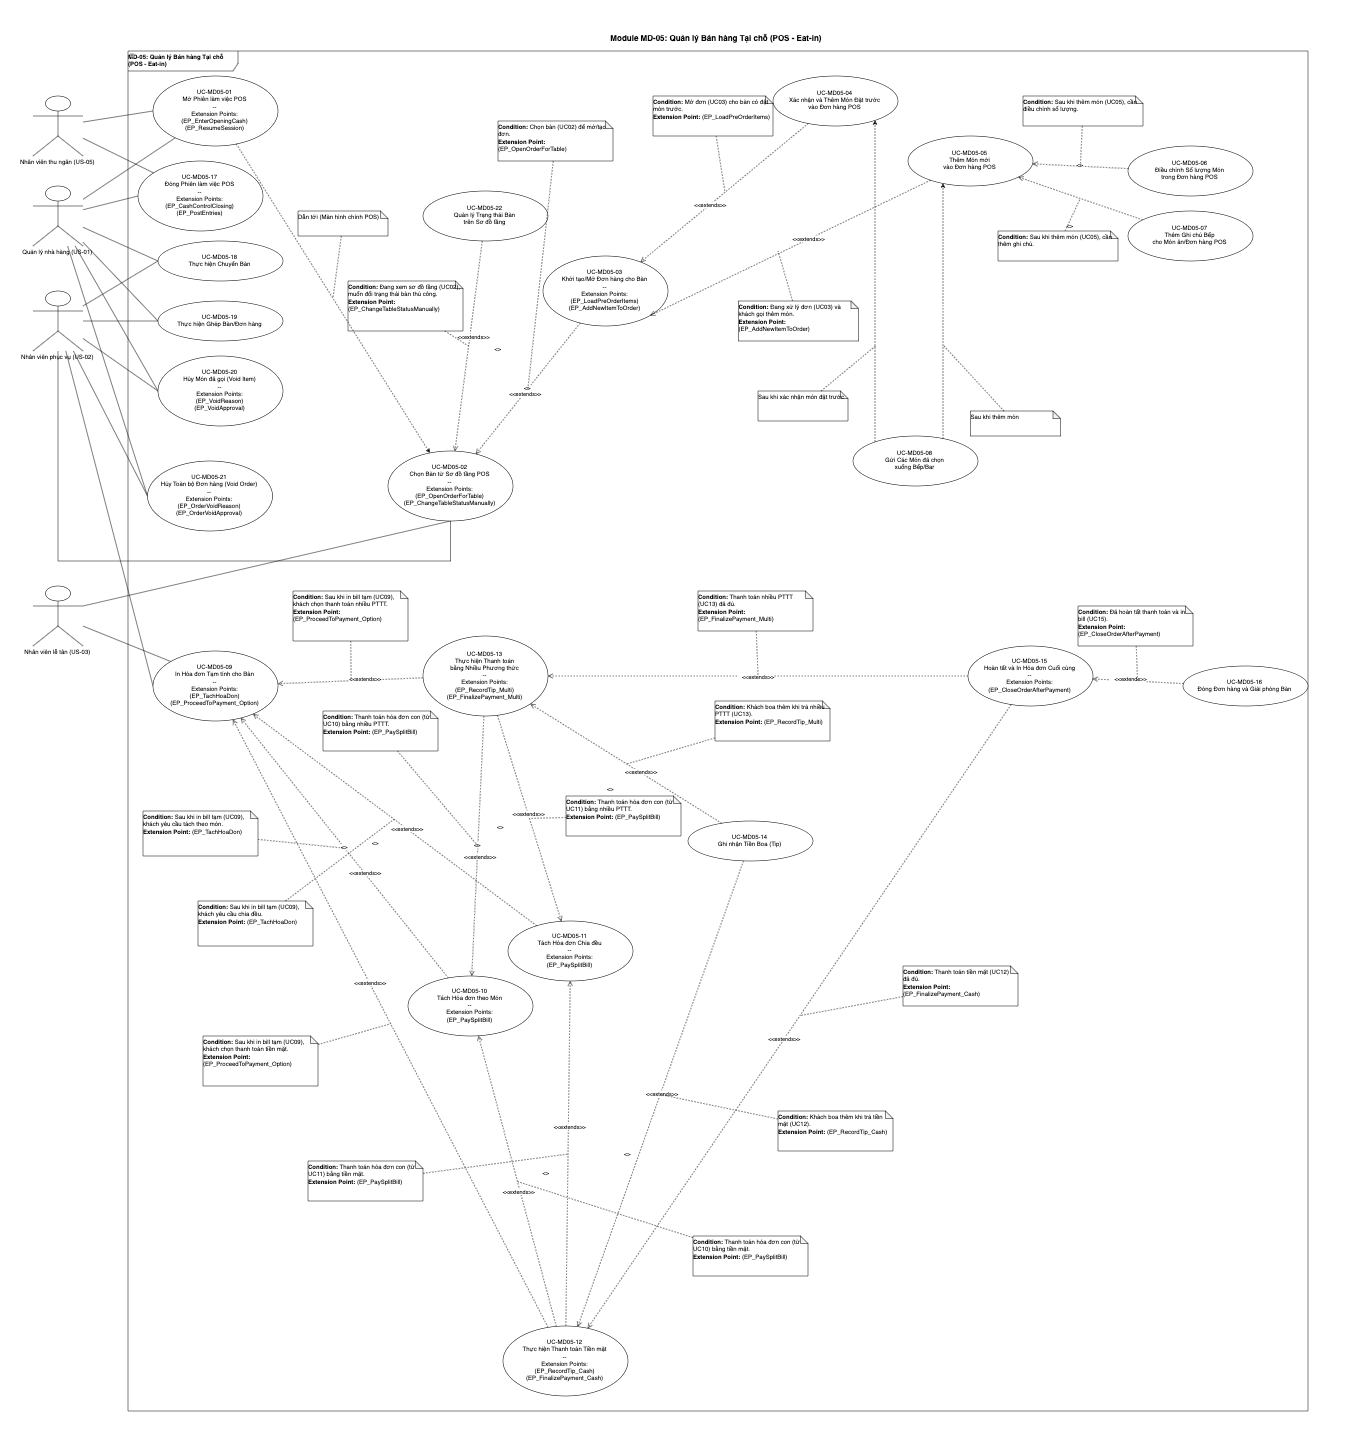
\includegraphics[width=15cm]{Sections/tong_quan/functional_spec/img/uc5.png}
    \vspace{0.5cm}
    \caption{Use case diagram cho Module MD-05}
    \label{fig:my_label}
\end{figure}

\begin{longtable}{|m{2cm}|m{2.5cm}|m{2cm}|m{4.5cm}|m{4cm}|}
\caption{Danh sách Yêu cầu Chức năng cho Module MD-05: Quản lý Bán hàng Tại chỗ (POS - Eat-in)} \label{tab:fr_md05_revised_v3_no_card} \\
\hline
\textbf{Mã Module} & \textbf{Mã Yêu cầu CN} & \textbf{Mã Người dùng} & \textbf{Tên Chức năng} & \textbf{Mô tả Ngắn} \\
\hline
\endhead % Header cho các trang tiếp theo
\hline
\endfoot % Footer cho bảng
\hline
\endlastfoot % Footer cho trang cuối cùng

MD-05 & FR-MD05-01 & US-05/US-01 & Mở Phiên làm việc POS & Cho phép Thu ngân/Quản lý bắt đầu phiên POS, nhập tiền mặt đầu ca. \\
\hline
MD-05 & FR-MD05-02 & US-02/US-03 & Chọn Bàn từ Sơ đồ tầng POS & Nhân viên chọn bàn trống hoặc bàn có khách/đặt trước từ sơ đồ tầng. \\
\hline
MD-05 & FR-MD05-03 & US-02 & Khởi tạo/Mở Đơn hàng cho Bàn & Hệ thống tạo đơn mới cho bàn trống hoặc mở đơn hiện có của bàn đang hoạt động/có đặt trước. \\
\hline
MD-05 & FR-MD05-04 & US-02 & Xác nhận và Thêm Món Đặt trước vào Đơn hàng POS & Nhân viên xem các món khách đã đặt trước (nếu có) và xác nhận thêm vào đơn hàng POS. \\
\hline
MD-05 & FR-MD05-05 & US-02 & Thêm Món mới vào Đơn hàng POS & Nhân viên chọn món từ menu POS để thêm vào đơn hàng hiện tại. \\
\hline
MD-05 & FR-MD05-06 & US-02 & Điều chỉnh Số lượng Món trong Đơn hàng POS & Nhân viên tăng/giảm số lượng một món đã có trong đơn hàng. \\
\hline
MD-05 & FR-MD05-07 & US-02 & Thêm Ghi chú Bếp cho Món ăn/Đơn hàng POS & Nhân viên thêm yêu cầu đặc biệt cho món hoặc cả đơn. \\
\hline
MD-05 & FR-MD05-08 & US-02 & Gửi Các Món đã chọn xuống Bếp/Bar & Nhân viên gửi các món mới thêm/món đặt trước đã xác nhận xuống bộ phận chuẩn bị. \\
\hline
MD-05 & FR-MD05-09 & US-02 & In Hóa đơn Tạm tính cho Bàn & Nhân viên in bill tạm tính (đã trừ cọc nếu có) cho khách kiểm tra. \\
\hline
MD-05 & FR-MD05-10 & US-02 & Tách Hóa đơn theo Món & Nhân viên chia hóa đơn của bàn theo từng món ăn cụ thể. \\
\hline
MD-05 & FR-MD05-11 & US-02 & Tách Hóa đơn Chia đều & Nhân viên chia đều tổng hóa đơn cho một số lượng người/phần nhất định. \\
\hline
MD-05 & FR-MD05-12 & US-02/US-05 & Thực hiện Thanh toán Tiền mặt & Nhân viên nhận tiền mặt, nhập số tiền nhận và hệ thống tính tiền thừa. \\
\hline
% FR-MD05-13 (Thanh toán thẻ) ĐÃ BỊ LOẠI BỎ
% Đánh số lại các FR tiếp theo
MD-05 & FR-MD05-13 & US-02/US-05 & Thực hiện Thanh toán bằng Nhiều Phương thức (Không bao gồm Thẻ) & Nhân viên nhận thanh toán cho một hóa đơn bằng cách kết hợp nhiều phương thức được hỗ trợ (ví dụ: Tiền mặt và Ví điện tử). \\
\hline
MD-05 & FR-MD05-14 & US-02/US-05 & Ghi nhận Tiền Boa (Tip) & Nhân viên nhập số tiền boa khách hàng trả thêm. \\
\hline
MD-05 & FR-MD05-15 & US-02/US-05 & Hoàn tất và In Hóa đơn Cuối cùng & Sau khi nhận đủ tiền, nhân viên xác nhận hoàn tất thanh toán và in hóa đơn/biên lai. \\
\hline
MD-05 & FR-MD05-16 & US-02 & Đóng Đơn hàng và Giải phóng Bàn & Nhân viên đóng đơn hàng đã thanh toán và cập nhật bàn thành trống. \\
\hline
MD-05 & FR-MD05-17 & US-05/US-01 & Đóng Phiên làm việc POS & Thu ngân/Quản lý kết thúc phiên, tổng kết, đối chiếu tiền mặt. \\
\hline
MD-05 & FR-MD05-18 & US-01/US-02 & Thực hiện Chuyển Bàn & Nhân viên chuyển toàn bộ đơn hàng từ bàn này sang bàn trống khác. \\
\hline
MD-05 & FR-MD05-19 & US-01/US-02 & Thực hiện Ghép Bàn/Đơn hàng & Nhân viên gộp nhiều đơn hàng từ các bàn khác nhau vào một bàn. \\
\hline
MD-05 & FR-MD05-20 & US-01/US-02 & Hủy Món đã gọi (Void Item) & Nhân viên hủy một món đã thêm vào đơn (có thể cần quyền). \\
\hline
MD-05 & FR-MD05-21 & US-01/US-02 & Hủy Toàn bộ Đơn hàng (Void Order) & Nhân viên hủy cả đơn hàng đang xử lý (có thể cần quyền). \\
\hline
MD-05 & FR-MD05-22 & US-02/ US-03 & Quản lý Trạng thái Bàn trên Sơ đồ tầng & Nhân viên có thể thay đổi thủ công trạng thái bàn (ví dụ: "Cần dọn", "Đang chờ") nếu cần. \\
\hline

\end{longtable}


\subsubsubsection{Mục tiêu và Phạm vi}
\label{sssec:md05_objectives_scope}
Mục tiêu chính của module MD-05 là:
\begin{itemize}
    \item \textbf{Tối ưu hóa quy trình phục vụ tại bàn:} Cung cấp một giao diện nhanh chóng, trực quan và dễ sử dụng cho nhân viên để nhận đơn, gửi bếp, và quản lý các yêu cầu của khách.
    \item \textbf{Quản lý bàn hiệu quả:} Hiển thị sơ đồ tầng trực quan với trạng thái bàn cập nhật theo thời gian thực, hỗ trợ việc xếp khách và theo dõi tình trạng phục vụ.
    \item \textbf{Đảm bảo tính chính xác của đơn hàng:} Giảm thiểu sai sót trong việc ghi nhận món ăn, số lượng, biến thể, và các yêu cầu đặc biệt của khách.
    \item \textbf{Tích hợp liền mạch với bếp/bar:} Gửi thông tin đơn hàng một cách chính xác và kịp thời đến các bộ phận chuẩn bị thông qua máy in hoặc Màn hình Hiển thị Bếp (KDS).
    \item \textbf{Linh hoạt trong thanh toán:} Hỗ trợ nhiều phương thức thanh toán, khả năng tách hóa đơn, và ghi nhận tiền boa.
    \item \textbf{Kiểm soát và báo cáo tài chính:} Ghi nhận tất cả các giao dịch, hỗ trợ đối chiếu tiền mặt cuối ca và cung cấp dữ liệu cho việc tạo các bút toán kế toán.
    \item \textbf{Nâng cao trải nghiệm khách hàng:} Thông qua việc phục vụ nhanh chóng, chính xác và khả năng đáp ứng linh hoạt các yêu cầu của khách.
\end{itemize}
Phạm vi của module bao gồm toàn bộ các hoạt động từ khi nhân viên mở phiên làm việc POS, quản lý đơn hàng cho từng bàn (tạo mới, thêm/sửa/hủy món, chuyển/ghép bàn), xử lý thanh toán, cho đến khi đóng phiên làm việc và tổng kết doanh thu.

\subsubsubsection{Đối tượng Sử dụng Chính}
\label{sssec:md05_primary_users}
Module này chủ yếu được sử dụng bởi các nhân viên tuyến đầu của nhà hàng:
\begin{itemize}
    \item \textbf{US-02 (Nhân viên phục vụ):} Là người dùng thường xuyên nhất, chịu trách nhiệm chính trong việc sử dụng sơ đồ tầng, nhận đơn hàng từ khách, thêm món, gửi yêu cầu bếp, và có thể cả việc nhận một phần thanh toán.
    \item \textbf{US-05 (Nhân viên thu ngân):} Chịu trách nhiệm mở và đóng phiên làm việc POS, xử lý các giao dịch thanh toán phức tạp, đối chiếu tiền mặt.
    \item \textbf{US-01 (Quản lý nhà hàng):} Có thể thực hiện tất cả các chức năng của nhân viên phục vụ và thu ngân, đồng thời có quyền thực hiện các hành động quản lý như hủy món/đơn hàng, chuyển/ghép bàn, và xem báo cáo phiên.
    \item \textbf{US-03 (Nhân viên lễ tân):} Có thể sử dụng sơ đồ tầng để xếp khách và mở đơn hàng ban đầu cho bàn.
\end{itemize}

\subsubsubsection{Các Chức năng Chính}
\label{sssec:md05_key_functionalities}
Module MD-05 cung cấp một bộ các chức năng toàn diện cho việc bán hàng tại chỗ, được mô tả chi tiết qua các Use Case sau:

\begin{itemize}
    \item \textbf{Quản lý Phiên làm việc POS (UC-MD05-01, UC-MD05-17):}
    \begin{itemize}
        \item Mở một phiên làm việc mới, tùy chọn nhập số dư tiền mặt đầu ca (UC-MD05-01).
        \item Đóng phiên làm việc cuối ca, tổng kết giao dịch, đối chiếu tiền mặt và ghi nhận bút toán (UC-MD05-17).
    \end{itemize}

    \item \textbf{Quản lý Bàn và Đơn hàng (UC-MD05-02, UC-MD05-03, UC-MD05-18, UC-MD05-19, UC-MD05-22):}
    \begin{itemize}
        \item Hiển thị và cho phép chọn bàn từ sơ đồ tầng trực quan với trạng thái cập nhật (UC-MD05-02).
        \item Khởi tạo một đơn hàng mới cho bàn trống/đặt trước hoặc mở lại đơn hàng đang hoạt động của bàn đã có khách (UC-MD05-03).
        \item Thực hiện chuyển toàn bộ đơn hàng từ bàn này sang bàn khác (UC-MD05-18).
        \item Thực hiện ghép các đơn hàng từ nhiều bàn vào một bàn đích duy nhất (UC-MD05-19).
        \item (Tùy chọn) Cho phép nhân viên thay đổi thủ công trạng thái của bàn trên sơ đồ tầng (ví dụ: "Cần dọn dẹp") (UC-MD05-22).
    \end{itemize}

    \item \textbf{Thao tác trên Đơn hàng (UC-MD05-04 đến UC-MD05-08, UC-MD05-20, UC-MD05-21):}
    \begin{itemize}
        \item Tự động tải và cho phép nhân viên xác nhận/thêm các món khách đã đặt trước online vào đơn hàng POS (UC-MD05-04).
        \item Thêm các món ăn/đồ uống mới vào đơn hàng từ menu trực quan, bao gồm cả việc chọn biến thể (UC-MD05-05).
        \item Điều chỉnh số lượng của một món đã có trong đơn hàng (UC-MD05-06).
        \item Thêm các ghi chú hoặc yêu cầu đặc biệt của khách cho từng món hoặc toàn bộ đơn hàng để gửi xuống bếp (UC-MD05-07).
        \item Gửi thông tin các món đã chọn (mới hoặc đặt trước) xuống các máy in bếp/bar hoặc màn hình KDS tương ứng (UC-MD05-08).
        \item Hủy một món cụ thể đã gọi trong đơn hàng (Void Item), có thể yêu cầu lý do và quyền quản lý (UC-MD05-20).
        \item Hủy toàn bộ một đơn hàng đang hoạt động (Void Order), thường yêu cầu quyền quản lý và lý do (UC-MD05-21).
    \end{itemize}

    \item \textbf{Xử lý Thanh toán (UC-MD05-09 đến UC-MD05-16):}
    \begin{itemize}
        \item In hóa đơn tạm tính cho khách kiểm tra, bao gồm cả việc trừ tiền đặt cọc đã thanh toán (nếu có) (UC-MD05-09).
        \item Tách hóa đơn theo từng món ăn cụ thể để nhiều người có thể trả riêng (UC-MD05-10).
        \item Tách hóa đơn bằng cách chia đều tổng giá trị cho một số lượng người nhất định (UC-MD05-11).
        \item Thực hiện thanh toán bằng tiền mặt, tính toán tiền trả lại (UC-MD05-12).
        \item Thực hiện thanh toán bằng nhiều phương thức khác nhau (không bao gồm thẻ tích hợp terminal) cho cùng một hóa đơn (UC-MD05-13).
        \item Ghi nhận số tiền boa (tip) do khách hàng trả thêm (UC-MD05-14).
        \item Sau khi nhận đủ thanh toán, hoàn tất giao dịch và in hóa đơn/biên lai cuối cùng cho khách (UC-MD05-15).
        \item Đóng đơn hàng đã thanh toán và giải phóng bàn, cập nhật trạng thái bàn thành trống (UC-MD05-16).
    \end{itemize}
\end{itemize}

\subsubsubsection{Tóm tắt Luồng Hoạt động Tổng thể}
\label{sssec:md05_overall_workflow}
Luồng hoạt động chính trong module Bán hàng Tại chỗ (POS) thường diễn ra như sau:
\begin{enumerate}
    \item \textbf{Bắt đầu ca làm việc:} Nhân viên thu ngân/Quản lý Mở Phiên làm việc POS (UC-MD05-01), nhập số dư tiền mặt đầu ca nếu cần.
    \item \textbf{Chọn bàn và mở đơn hàng:}
        \begin{itemize}
            \item Nhân viên phục vụ Chọn Bàn từ Sơ đồ tầng POS (UC-MD05-02) dựa trên tình trạng bàn (trống, đặt trước).
            \item Hệ thống Khởi tạo/Mở Đơn hàng cho Bàn (UC-MD05-03).
        \end{itemize}
    \item \textbf{Nhận yêu cầu gọi món từ khách:}
        \begin{itemize}
            \item Nếu bàn có đặt món trước, nhân viên Xác nhận và Thêm Món Đặt trước vào Đơn hàng POS (UC-MD05-04).
            \item Nhân viên Thêm Món mới vào Đơn hàng POS (UC-MD05-05) theo yêu cầu của khách.
            \item Điều chỉnh Số lượng Món (UC-MD05-06) hoặc Thêm Ghi chú Bếp (UC-MD05-07) nếu cần.
            \item Sau mỗi lượt gọi món hoặc khi cần, nhân viên Gửi Các Món đã chọn xuống Bếp/Bar (UC-MD05-08).
        \end{itemize}
    \item \textbf{Quản lý đơn hàng trong quá trình phục vụ (nếu có):}
        \begin{itemize}
            \item Khách yêu cầu chuyển bàn: Nhân viên Thực hiện Chuyển Bàn (UC-MD05-18).
            \item Nhiều nhóm khách muốn ngồi chung: Nhân viên Thực hiện Ghép Bàn/Đơn hàng (UC-MD05-19).
            \item Khách đổi ý/nhân viên nhập sai: Nhân viên Hủy Món đã gọi (Void Item) (UC-MD05-20).
            \item Khách rời đi/lỗi nghiêm trọng: Nhân viên/Quản lý Hủy Toàn bộ Đơn hàng (Void Order) (UC-MD05-21).
            \item Cập nhật trạng thái bàn thủ công (ví dụ: "Cần dọn"): Nhân viên Quản lý Trạng thái Bàn trên Sơ đồ tầng (UC-MD05-22).
        \end{itemize}
    \item \textbf{Khách yêu cầu thanh toán:}
        \begin{itemize}
            \item Nhân viên In Hóa đơn Tạm tính cho Bàn (UC-MD05-09).
            \item Nếu khách yêu cầu trả riêng: Nhân viên Tách Hóa đơn theo Món (UC-MD05-10) hoặc Tách Hóa đơn Chia đều (UC-MD05-11).
            \item Nhân viên nhận thanh toán bằng các phương thức: Thực hiện Thanh toán Tiền mặt (UC-MD05-12), hoặc Thực hiện Thanh toán bằng Nhiều Phương thức (UC-MD05-13).
            \item Nếu khách boa: Nhân viên Ghi nhận Tiền Boa (Tip) (UC-MD05-14).
        \end{itemize}
    \item \textbf{Hoàn tất giao dịch:}
        \begin{itemize}
            \item Sau khi nhận đủ tiền, nhân viên Hoàn tất và In Hóa đơn Cuối cùng (UC-MD05-15).
            \item Cuối cùng, nhân viên Đóng Đơn hàng và Giải phóng Bàn (UC-MD05-16).
        \end{itemize}
    \item \textbf{Kết thúc ca làm việc:} Nhân viên thu ngân/Quản lý Đóng Phiên làm việc POS (UC-MD05-17), tổng kết và đối chiếu.
\end{enumerate}
Module MD-05 là trung tâm của các hoạt động dịch vụ tại nhà hàng, đảm bảo quy trình diễn ra mượt mà, chính xác và hiệu quả.

\subsubsection{Module MD-06: Quản lý Bán mang về (POS - Takeout)}

\begin{longtable}{|m{2cm}|m{2.5cm}|m{2.5cm}|m{4.5cm}|m{4cm}|}
\caption{Danh sách Yêu cầu Chức năng cho Module MD-06: Quản lý Bán mang về (POS - Takeout)} \label{tab:fr_md06} \\
\hline
\textbf{Mã Module} & \textbf{Mã Yêu cầu CN} & \textbf{Mã Người dùng} & \textbf{Tên Chức năng} & \textbf{Mô tả Ngắn} \\
\hline
\endhead % Header cho các trang tiếp theo

\hline
\endfoot % Footer cho bảng

\hline
\endlastfoot % Footer cho trang cuối cùng

MD-06 & FR-MD06-01 & US-02, US-05 & Chọn Chế độ Bán Mang về & Cho phép nhân viên chọn một chế độ/giao diện riêng biệt trên POS dành cho việc tạo đơn hàng mang về, bỏ qua bước chọn bàn. \\
\hline
MD-06 & FR-MD06-02 & US-02, US-05 & Tạo Đơn hàng Mang về & Khởi tạo một đơn hàng mới trong chế độ mang về, không liên kết với bàn cụ thể. \\
\hline
MD-06 & FR-MD06-03 & US-02, US-05 & (Tùy chọn) Liên kết Khách hàng & Cho phép tìm kiếm và liên kết đơn hàng mang về với một khách hàng đã có trong hệ thống hoặc tạo nhanh thông tin khách hàng mới (Tên, SĐT). \\
\hline
MD-06 & FR-MD06-04 & US-02, US-05 & Thêm món vào Đơn hàng Mang về & Cho phép nhân viên thêm các món ăn/đồ uống vào đơn hàng mang về, tương tự như cách thêm món cho đơn hàng tại bàn (UC-MD05-05). \\
\hline
MD-06 & FR-MD06-05 & US-02, US-05 & Xử lý Ghi chú cho Đơn Mang về & Cho phép thêm ghi chú đặc biệt cho các món hoặc toàn bộ đơn hàng mang về (ví dụ: "Gói kỹ", "Thêm tương ớt"). Tương tự UC-MD05-06. \\
\hline
MD-06 & FR-MD06-06 & US-02, US-05 & Gửi đơn Mang về xuống Bếp/Bar & Gửi thông tin các món cần chuẩn bị cho đơn hàng mang về đến các bộ phận liên quan (Bếp/Bar). Tương tự UC-MD05-07, có thể cần đánh dấu là đơn "Takeout". \\
\hline
MD-06 & FR-MD06-07 & US-02, US-05, System & Áp dụng Đặt cọc (Nếu Đặt trước Online) & Nếu đơn hàng mang về này được khách đặt trước online (qua một luồng khác) và có đặt cọc, hệ thống cần áp dụng tiền cọc vào hóa đơn. (Logic tương tự UC-MD05-09 nhưng áp dụng cho đơn takeout). \\
\hline
MD-06 & FR-MD06-08 & US-02, US-05 & Thanh toán Đơn hàng Mang về & Cho phép nhận thanh toán ngay tại quầy cho đơn hàng mang về bằng các phương thức khác nhau. Tương tự UC-MD05-11. \\
\hline
MD-06 & FR-MD06-09 & US-02, US-05 & In Hóa đơn/Phiếu thu Mang về & In hóa đơn/phiếu thu cho khách hàng sau khi thanh toán thành công. Có thể cần mẫu in khác biệt cho đơn mang về. \\
\hline
MD-06 & FR-MD06-10 & US-02, US-05 & Đóng Đơn hàng Mang về & Hoàn tất và đóng đơn hàng mang về sau khi khách đã thanh toán và nhận hàng. \\
\hline

\end{longtable}

\subsubsection{Module MD-07: Quản lý Giao hàng (POS - Delivery)}
Module Quản lý Giao hàng (MD-07) là một thành phần quan trọng của hệ thống Point of Sale (POS), được thiết kế đặc biệt để hỗ trợ nhà hàng quản lý các đơn hàng mà khách yêu cầu giao đến một địa chỉ cụ thể. Module này tập trung vào việc thu thập thông tin khách hàng và địa chỉ giao hàng, xử lý đơn hàng, và đặc biệt là tích hợp với dịch vụ quản lý giao hàng của bên thứ ba (trong trường hợp này là Shipday) để tự động hóa việc gửi yêu cầu giao hàng và theo dõi trạng thái.



\begin{figure}[H]
    \centering
    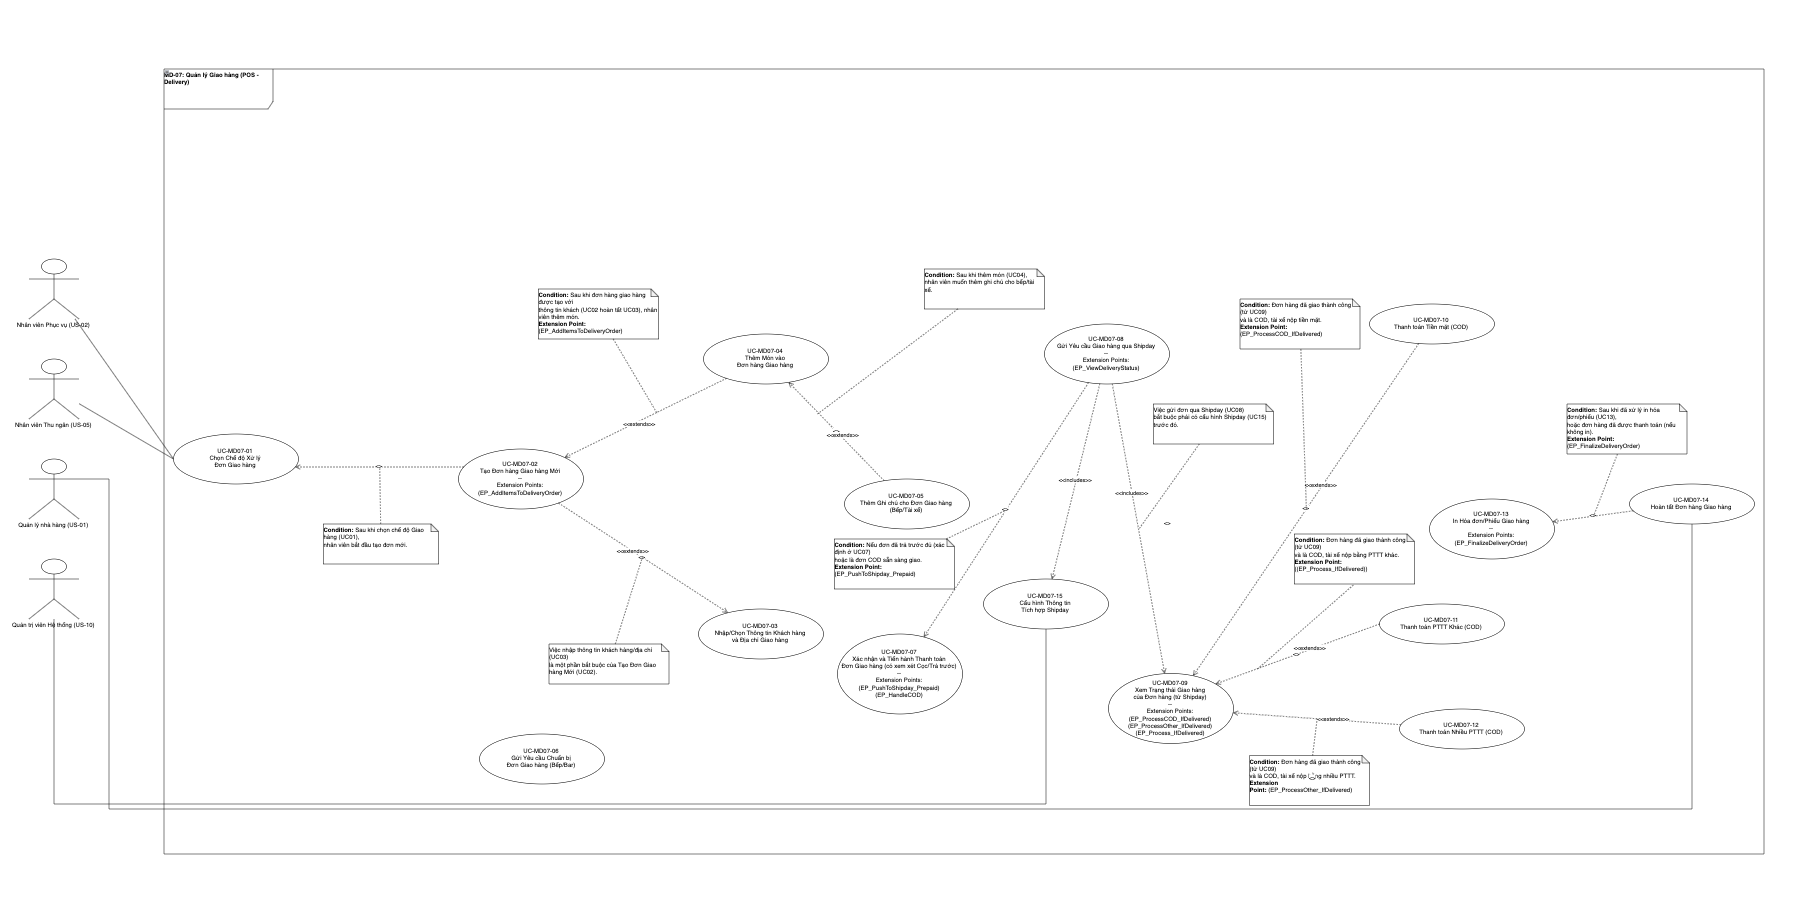
\includegraphics[width=15cm]{Sections/tong_quan/functional_spec/img/uc7.png}
    \vspace{0.5cm}
    \caption{Use case diagram cho Module MD-07}
    \label{fig:my_label}
\end{figure}

\begin{longtable}{|m{2cm}|m{2.5cm}|m{2.5cm}|m{4.5cm}|m{4cm}|}
\caption{Danh sách Yêu cầu Chức năng cho Module MD-07: Quản lý Giao hàng (POS - Delivery)} \label{tab:fr_md07_revised_v2} \\
\hline
\textbf{Mã Module} & \textbf{Mã Yêu cầu CN} & \textbf{Mã Người dùng} & \textbf{Tên Chức năng} & \textbf{Mô tả Ngắn} \\
\hline
\endhead % Header cho các trang tiếp theo
\hline
\endfoot % Footer cho bảng
\hline
\endlastfoot % Footer cho trang cuối cùng

MD-07 & FR-MD07-01 & US-02, US-05 & Chọn Chế độ Xử lý Đơn Giao hàng & Nhân viên chọn chế độ/giao diện riêng trên POS cho đơn giao hàng. \\
\hline
MD-07 & FR-MD07-02 & US-02, US-05 & Tạo Đơn hàng Giao hàng Mới & Nhân viên khởi tạo đơn hàng mới, yêu cầu liên kết thông tin khách hàng giao hàng. \\
\hline
MD-07 & FR-MD07-03 & US-02, US-05 & Nhập/Chọn Thông tin Khách hàng và Địa chỉ Giao hàng & Nhân viên tìm/chọn khách hàng có sẵn hoặc nhập mới Tên, SĐT, Địa chỉ giao hàng chi tiết. \\
\hline
MD-07 & FR-MD07-04 & US-02, US-05 & Thêm Món vào Đơn hàng Giao hàng & Nhân viên thêm món ăn/đồ uống vào đơn hàng giao đi. \\
\hline
MD-07 & FR-MD07-05 & US-02, US-05 & Thêm Ghi chú cho Đơn Giao hàng (Bếp/Tài xế) & Nhân viên thêm ghi chú cho bếp hoặc ghi chú cho tài xế giao hàng. \\
\hline
MD-07 & FR-MD07-06 & US-02, US-05 & Gửi Yêu cầu Chuẩn bị Đơn Giao hàng (Bếp/Bar) & Nhân viên gửi thông tin món cần chuẩn bị xuống bếp/bar, có đánh dấu "Delivery". \\
\hline
MD-07 & FR-MD07-07 & US-02, US-05 & Xác nhận và Tiến hành Thanh toán Đơn Giao hàng (có xem xét Cọc/Trả trước) & Nhân viên vào màn hình thanh toán, nơi hệ thống đã tự động áp dụng cọc/trả trước (nếu đơn hàng được đặt online và có trả trước). \\
\hline
MD-07 & FR-MD07-08 & US-02, US-05 & Gửi Yêu cầu Giao hàng qua Shipday & Sau khi đơn hàng sẵn sàng, nhân viên kích hoạt gửi thông tin đơn hàng sang Shipday. \\
\hline
MD-07 & FR-MD07-09 & US-02, US-05, US-01 & Xem Trạng thái Giao hàng của Đơn hàng (từ Shipday) & Nhân viên xem trạng thái giao hàng (Đã gán tài xế, Đang giao...) được cập nhật từ Shipday trên chi tiết đơn hàng. \\
\hline
MD-07 & FR-MD07-10 & US-02, US-05 & Thực hiện Thanh toán Tiền mặt cho Đơn Giao hàng (Nếu COD) & Nhân viên nhận tiền mặt COD từ tài xế và ghi nhận vào hệ thống. \\
\hline
MD-07 & FR-MD07-11 & US-02, US-05 & Ghi nhận Thanh toán bằng Phương thức Khác (Không Thẻ) cho Đơn Giao hàng (Nếu COD) & Nhân viên ghi nhận thanh toán COD bằng phương thức khác được hỗ trợ. \\
\hline
MD-07 & FR-MD07-12 & US-02, US-05 & Thực hiện Thanh toán Đơn Giao hàng bằng Nhiều Phương thức (Không Thẻ, Nếu COD) & Nhân viên nhận thanh toán COD bằng nhiều phương thức. \\
\hline
MD-07 & FR-MD07-13 & US-02, US-05 & In Hóa đơn/Phiếu Giao hàng & Nhân viên in hóa đơn/phiếu giao hàng để tài xế sử dụng. \\
\hline
MD-07 & FR-MD07-14 & US-02, US-05 & Hoàn tất Đơn hàng Giao hàng & Nhân viên đóng đơn hàng giao đi sau khi đã giao thành công và (nếu COD) đã nhận đủ thanh toán. \\
\hline
MD-07 & FR-MD07-15 & US-01/US-10 & Cấu hình Thông tin Tích hợp Shipday & Quản trị viên/Quản lý cấu hình các tham số kết nối API và Shipday. \\
\hline

\end{longtable}


\subsubsubsection{Mục tiêu và Phạm vi}
\label{sssec:md07_objectives_scope}
Mục tiêu chính của module MD-07 bao gồm:
\begin{itemize}
    \item \textbf{Quản lý hiệu quả đơn hàng giao đi:} Cung cấp một quy trình đầy đủ từ việc nhận đơn, nhập thông tin khách hàng và địa chỉ, xử lý món ăn, cho đến khi gửi đơn cho đơn vị vận chuyển và theo dõi.
    \item \textbf{Tích hợp liền mạch với dịch vụ giao hàng bên ngoài (Shipday):} Tự động hóa việc gửi thông tin đơn hàng sang Shipday để tìm tài xế và quản lý quá trình giao hàng.
    \item \textbf{Theo dõi trạng thái giao hàng:} Cập nhật trạng thái đơn hàng trong hệ thống dựa trên thông tin phản hồi từ Shipday.
    \item \textbf{Xử lý thanh toán linh hoạt cho đơn giao hàng:} Hỗ trợ các hình thức thanh toán như trả trước online hoặc thu tiền khi nhận hàng (COD).
    \item \textbf{Cung cấp thông tin chính xác cho các bên liên quan:} Đảm bảo bếp/bar nhận đúng yêu cầu chuẩn bị, tài xế có đủ thông tin giao hàng, và nhân viên nhà hàng có thể theo dõi quá trình.
    \item \textbf{Nâng cao trải nghiệm khách hàng:} Thông qua việc giao hàng đúng hẹn và thông tin rõ ràng.
\end{itemize}
Phạm vi của module bao gồm từ việc nhân viên chọn chế độ xử lý đơn giao hàng, tạo đơn hàng, nhập thông tin chi tiết, gửi yêu cầu chuẩn bị, gửi đơn sang Shipday, theo dõi trạng thái, cho đến khi xử lý thanh toán COD (nếu có) và hoàn tất đơn hàng.

\subsubsubsection{Đối tượng Sử dụng Chính}
\label{sssec:md07_primary_users}
Các đối tượng người dùng và hệ thống chính tương tác với module này bao gồm:
\begin{itemize}
    \item \textbf{US-02 (Nhân viên phục vụ) / US-05 (Nhân viên thu ngân):} Là những người trực tiếp nhận yêu cầu đặt hàng giao đi, tạo đơn hàng trên POS, nhập thông tin khách hàng, địa chỉ, món ăn, và gửi yêu cầu giao hàng sang Shipday.
    \item \textbf{US-01 (Quản lý nhà hàng):} Có thể thực hiện tất cả các chức năng của nhân viên, giám sát quá trình, xử lý các trường hợp đặc biệt, và cấu hình tích hợp.
    \item \textbf{US-10 (Quản trị viên Hệ thống):} Chịu trách nhiệm cấu hình kỹ thuật cho việc tích hợp API với Shipday.
    \item \textbf{System (Hệ thống Shipday):} Hệ thống tự động hóa nhiều bước, trong khi Shipday là hệ thống bên ngoài chịu trách nhiệm quản lý đội xe và quá trình giao hàng thực tế.
\end{itemize}

\subsubsubsection{Các Chức năng Chính}
\label{sssec:md07_key_functionalities}
Module MD-07 cung cấp một chuỗi các chức năng để quản lý toàn diện quy trình giao hàng, được mô tả chi tiết qua các Use Case sau:

\begin{itemize}
    \item \textbf{Khởi tạo và Chuẩn bị Đơn hàng Giao hàng (UC-MD07-01 đến UC-MD07-06):}
    \begin{itemize}
        \item Cho phép nhân viên chọn chế độ hoạt động hoặc giao diện dành riêng cho việc xử lý đơn hàng giao đi (UC-MD07-01).
        \item Nhân viên khởi tạo một đơn hàng POS mới, được hệ thống tự động đánh dấu là loại hình "Giao hàng" (UC-MD07-02).
        \item Yêu cầu nhân viên bắt buộc phải nhập hoặc chọn thông tin khách hàng và địa chỉ giao hàng chi tiết cho đơn hàng (UC-MD07-03).
        \item Thêm các món ăn/đồ uống từ thực đơn POS vào đơn hàng giao đi (UC-MD07-04, tương tự UC-MD05-05).
        \item Thêm các ghi chú đặc biệt cho bếp (về món ăn) hoặc cho tài xế (về việc giao hàng) (UC-MD07-05, tương tự UC-MD05-07 nhưng có thêm ghi chú cho tài xế).
        \item Gửi thông tin các món cần chuẩn bị của đơn hàng giao đi xuống các máy in bếp/bar hoặc màn hình KDS, có chỉ dẫn rõ là đơn "Delivery" (UC-MD07-06, tương tự UC-MD05-08 nhưng có thêm thông tin "Delivery").
    \end{itemize}

    \item \textbf{Xử lý Thanh toán và Tích hợp Giao hàng (UC-MD07-07, UC-MD07-08, UC-MD07-10, UC-MD07-11, UC-MD07-12):}
    \begin{itemize}
        \item Trước khi vào màn hình thanh toán hoặc xác nhận đơn, hệ thống tự động kiểm tra và áp dụng (trừ đi) các khoản tiền đặt cọc hoặc thanh toán trước (nếu có) cho đơn hàng giao đi (UC-MD07-07).
        \item Gửi thông tin chi tiết của đơn hàng (bao gồm địa chỉ, thông tin khách, món ăn, số tiền COD nếu có) đến hệ thống quản lý giao hàng Shipday thông qua API (UC-MD07-08).
        \item Đối với đơn hàng COD, cho phép nhân viên ghi nhận việc đã nhận tiền mặt từ tài xế (UC-MD07-10, tương tự UC-MD05-12).
        \item Ghi nhận việc tài xế nộp tiền COD bằng các phương thức khác tiền mặt (ví dụ: chuyển khoản) (UC-MD07-11, tương tự UC-MD06-09 cho Takeout).
        \item (Tùy chọn) Ghi nhận việc tài xế nộp tiền COD bằng nhiều phương thức kết hợp (UC-MD07-12, tương tự UC-MD05-14).
    \end{itemize}

    \item \textbf{Theo dõi và Hoàn tất Đơn hàng Giao hàng (UC-MD07-09, UC-MD07-13, UC-MD07-14):}
    \begin{itemize}
        \item Hiển thị trạng thái giao hàng mới nhất của đơn hàng (ví dụ: "Đang giao", "Đã giao thành công") được hệ thống tự động cập nhật từ Shipday (thường qua webhook) (UC-MD07-09).
        \item In hóa đơn hoặc phiếu giao hàng chi tiết cho đơn hàng giao đi, để đính kèm gói hàng hoặc giao cho khách (UC-MD07-13, tương tự UC-MD06-11).
        \item Chính thức đóng đơn hàng giao đi trong hệ thống sau khi đã xác nhận giao hàng thành công và tất cả các vấn đề thanh toán đã được xử lý (UC-MD07-14, tương tự UC-MD06-12).
    \end{itemize}

    \item \textbf{Cấu hình Tích hợp (UC-MD07-15):}
    \begin{itemize}
        \item Cho phép Quản lý/Quản trị viên thiết lập và quản lý các tham số cần thiết để kết nối và trao đổi dữ liệu với nền tảng Shipday, bao gồm API Key (UC-MD07-15).
    \end{itemize}
\end{itemize}

\subsubsubsection{Tóm tắt Luồng Hoạt động Tổng thể}
\label{sssec:md07_overall_workflow}
Luồng hoạt động chính trong module Quản lý Giao hàng (POS - Delivery) thường diễn ra như sau:
\begin{enumerate}
    \item \textbf{Cấu hình ban đầu:} Quản lý/Quản trị viên Cấu hình Thông tin Tích hợp Shipday (UC-MD07-15).
    \item \textbf{Nhận và tạo đơn hàng giao đi:}
        \begin{itemize}
            \item Nhân viên Chọn Chế độ Xử lý Đơn Giao hàng (UC-MD07-01).
            \item Hệ thống yêu cầu, và nhân viên Tạo Đơn hàng Giao hàng Mới kèm theo việc Nhập/Chọn Thông tin Khách hàng và Địa chỉ Giao hàng (UC-MD07-02, UC-MD07-03).
            \item Nhân viên Thêm Món vào Đơn hàng Giao hàng (UC-MD07-04) và Thêm Ghi chú cho Đơn Giao hàng (Bếp/Tài xế) (UC-MD07-05).
            \item Nhân viên Gửi Yêu cầu Chuẩn bị Đơn Giao hàng (Bếp/Bar) (UC-MD07-06).
        \end{itemize}
    \item \textbf{Xử lý thanh toán và gửi giao hàng:}
        \begin{itemize}
            \item Nhân viên tiến hành xác nhận đơn, hệ thống tự động xem xét và áp dụng các khoản Cọc/Trả trước (UC-MD07-07).
            \item Sau khi đơn hàng sẵn sàng (đã chuẩn bị, thông tin thanh toán rõ ràng), nhân viên Gửi Yêu cầu Giao hàng qua Shipday (UC-MD07-08).
        \end{itemize}
    \item \textbf{Theo dõi và hoàn tất:}
        \begin{itemize}
            \item Nhân viên có thể Xem Trạng thái Giao hàng của Đơn hàng (từ Shipday) (UC-MD07-09) được cập nhật tự động.
            \item Khi cần, nhân viên In Hóa đơn/Phiếu Giao hàng (UC-MD07-13).
            \item Nếu là đơn COD và đã giao thành công, nhân viên ghi nhận thanh toán từ tài xế: Tiền mặt (UC-MD07-10), Phương thức Khác (UC-MD07-11), hoặc Nhiều Phương thức (UC-MD07-12).
            \item Cuối cùng, sau khi giao thành công và thanh toán hoàn tất, nhân viên hoặc hệ thống Hoàn tất Đơn hàng Giao hàng (UC-MD07-14).
        \end{itemize}
\end{enumerate}
Module MD-07 kết hợp các chức năng POS nội bộ với khả năng tích hợp mạnh mẽ của Shipday, tạo nên một giải pháp toàn diện cho việc quản lý dịch vụ giao hàng của nhà hàng.


\subsubsection{Module MD-08: Tích hợp Bếp (Kitchen Integration)}
Module Quản lý Giao hàng (MD-07) là một thành phần quan trọng của hệ thống Point of Sale (POS), được thiết kế đặc biệt để hỗ trợ nhà hàng quản lý các đơn hàng mà khách yêu cầu giao đến một địa chỉ cụ thể. Module này tập trung vào việc thu thập thông tin khách hàng và địa chỉ giao hàng, xử lý đơn hàng, và đặc biệt là tích hợp với dịch vụ quản lý giao hàng của bên thứ ba (trong trường hợp này là Shipday) để tự động hóa việc gửi yêu cầu giao hàng và theo dõi trạng thái.

Module Tích hợp Bếp (MD-08) đóng vai trò cầu nối quan trọng giữa bộ phận phục vụ (thông qua hệ thống POS) và bộ phận bếp/bar. Mục tiêu chính của module này là đảm bảo thông tin đơn hàng được truyền tải một cách chính xác, kịp thời và hiệu quả đến các nhân viên bếp, giúp họ chuẩn bị món ăn đúng theo yêu cầu và tối ưu hóa quy trình làm việc trong bếp. Module này có thể được triển khai dưới dạng Màn hình Hiển thị Bếp (Kitchen Display System - KDS) hoặc thông qua việc sử dụng máy in bếp truyền thống.


\begin{figure}[H]
    \centering
    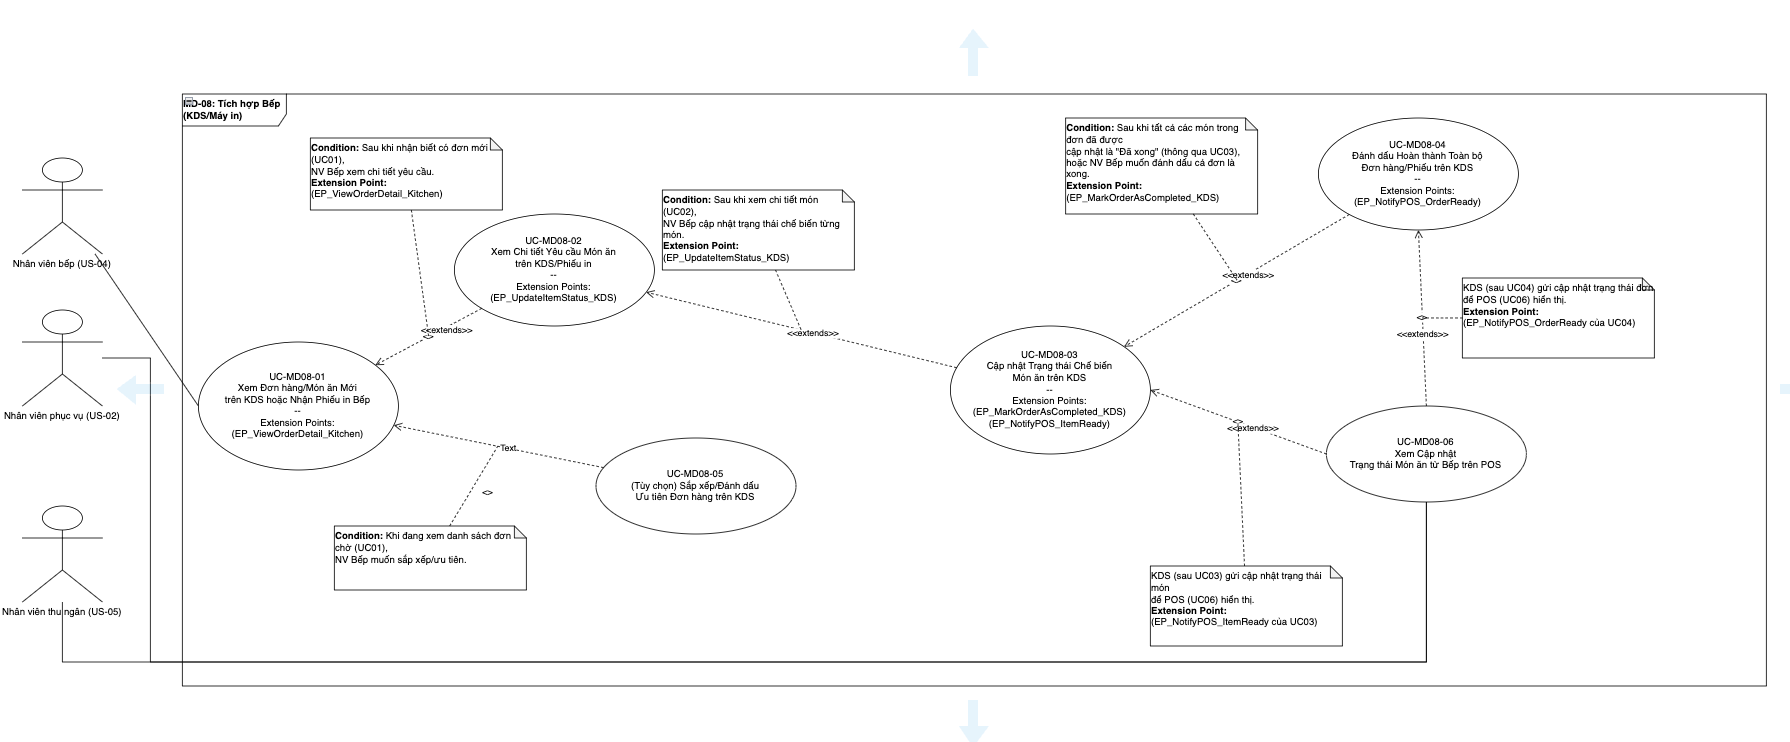
\includegraphics[width=15cm]{Sections/tong_quan/functional_spec/img/uc8.png}
    \vspace{0.5cm}
    \caption{Use case diagram cho Module MD-08}
    \label{fig:my_label}
\end{figure}

\begin{longtable}{|m{2cm}|m{2.5cm}|m{2.5cm}|m{4.5cm}|m{4cm}|}
\caption{Danh sách Yêu cầu Chức năng cho Module MD-08: Tích hợp Bếp (Kitchen Integration)} \label{tab:fr_md08_revised_v2} \\
\hline
\textbf{Mã Module} & \textbf{Mã Yêu cầu CN} & \textbf{Mã Người dùng} & \textbf{Tên Chức năng} & \textbf{Mô tả Ngắn} \\
\hline
\endhead % Header cho các trang tiếp theo
\hline
\endfoot % Footer cho bảng
\hline
\endlastfoot % Footer cho trang cuối cùng

MD-08 & FR-MD08-01 & US-04 & Xem Đơn hàng/Món ăn Mới trên KDS/Máy in Bếp & Nhân viên bếp xem các đơn hàng/món ăn mới được gửi đến KDS hoặc nhận phiếu in từ máy in bếp. (Việc gửi đi là kết quả của FR-MD05-08, FR-MD06-06, FR-MD07-06). \\
\hline
MD-08 & FR-MD08-02 & US-04 & Xem Chi tiết Yêu cầu Món ăn trên KDS/Phiếu in & Nhân viên bếp đọc thông tin chi tiết của từng món cần chuẩn bị: tên, số lượng, biến thể, ghi chú đặc biệt. \\
\hline
MD-08 & FR-MD08-03 & US-04 & Cập nhật Trạng thái Chế biến Món ăn trên KDS & Nhân viên bếp tương tác với KDS để đánh dấu trạng thái chế biến của món ăn (ví dụ: Bắt đầu làm, Đã xong). \\
\hline
MD-08 & FR-MD08-04 & US-04 & Đánh dấu Hoàn thành Toàn bộ Đơn hàng/Phiếu trên KDS & Nhân viên bếp đánh dấu toàn bộ các món trong một đơn hàng/phiếu đã được chuẩn bị xong trên KDS. \\
\hline
MD-08 & FR-MD08-05 & US-04 & Sắp xếp/Đánh dấu Ưu tiên Đơn hàng trên KDS & Nhân viên bếp thay đổi thứ tự hoặc đánh dấu ưu tiên cho các đơn hàng/phiếu trên KDS. \\
\hline
MD-08 & FR-MD08-06 & US-02/US-05 & Xem Cập nhật Trạng thái Món ăn từ Bếp trên POS & Nhân viên phục vụ/thu ngân xem được thông tin món nào đã sẵn sàng từ bếp (nếu KDS có gửi cập nhật về POS). \\
\hline

\end{longtable}


\subsubsubsection{Mục tiêu và Phạm vi}
\label{sssec:md08_objectives_scope}
Mục tiêu chính của module MD-08 là:
\begin{itemize}
    \item \textbf{Truyền tải chính xác yêu cầu món ăn:} Đảm bảo mọi chi tiết của đơn hàng (tên món, số lượng, biến thể, ghi chú đặc biệt) được gửi từ POS đến bếp một cách đầy đủ và không sai sót.
    \item \textbf{Tối ưu hóa quy trình làm việc trong bếp:} Giúp nhân viên bếp dễ dàng tiếp nhận, xem, quản lý và theo dõi tiến độ chuẩn bị các món ăn.
    \item \textbf{Giảm thiểu sai sót và nhầm lẫn:} Hạn chế việc trao đổi thông tin bằng miệng hoặc giấy tờ dễ thất lạc, từ đó giảm lỗi trong quá trình chế biến.
    \item \textbf{Cải thiện thời gian phục vụ:} Giúp bếp nhận yêu cầu nhanh hơn và quản lý thứ tự ưu tiên hiệu quả hơn (đặc biệt với KDS).
    \item \textbf{(Nếu dùng KDS) Cung cấp khả năng theo dõi và cập nhật trạng thái:} Cho phép nhân viên bếp đánh dấu trạng thái chế biến (đang làm, đã xong) và (tùy chọn) đồng bộ thông tin này ngược lại cho nhân viên phục vụ.
    \item \textbf{Hỗ trợ định tuyến thông minh:} Đảm bảo các món ăn được gửi đến đúng trạm chuẩn bị (ví dụ: món chính gửi bếp chính, đồ uống gửi quầy bar) nếu nhà hàng có nhiều khu vực bếp/bar.
\end{itemize}
Phạm vi của module bao gồm việc tiếp nhận yêu cầu món ăn từ hệ thống POS (MD-05, MD-06, MD-07), hiển thị thông tin chi tiết cho nhân viên bếp, và (nếu sử dụng KDS) cho phép nhân viên bếp tương tác để cập nhật trạng thái chế biến. Nó không bao gồm việc quản lý công thức, định lượng nguyên vật liệu, hay các chức năng quản lý kho chi tiết (thuộc các module khác).

\subsubsubsection{Đối tượng Sử dụng Chính}
\label{sssec:md08_primary_users}
Đối tượng người dùng chính của module này là:
\begin{itemize}
    \item \textbf{US-04 (Nhân viên bếp):} Là người trực tiếp sử dụng KDS hoặc nhận phiếu in từ máy in bếp để xem yêu cầu, chuẩn bị món ăn, và (nếu có KDS) cập nhật trạng thái chế biến.
\end{itemize}
Các đối tượng khác tương tác gián tiếp:
\begin{itemize}
    \item \textbf{US-02 (Nhân viên phục vụ) / US-05 (Nhân viên thu ngân):} Là người gửi yêu cầu chuẩn bị món từ POS. Họ cũng có thể (tùy chọn) nhận được cập nhật trạng thái món ăn từ KDS (UC-MD08-06).
    \item \textbf{US-01 (Quản lý nhà hàng) / US-10 (Quản trị viên Hệ thống):} Chịu trách nhiệm cấu hình máy in bếp, KDS, và các quy tắc định tuyến.
\end{itemize}

\subsubsubsection{Các Chức năng Chính}
\label{sssec:md08_key_functionalities}
Module MD-08 cung cấp các chức năng thiết yếu cho việc vận hành bếp, được mô tả chi tiết qua các Use Case sau:

\begin{itemize}
    \item \textbf{Tiếp nhận và Hiển thị Yêu cầu (UC-MD08-01, UC-MD08-02):}
    \begin{itemize}
        \item Nhân viên bếp xem các đơn hàng/món ăn mới xuất hiện trên Màn hình Hiển thị Bếp (KDS) hoặc nhận phiếu yêu cầu được in ra từ máy in bếp (UC-MD08-01).
        \item Nhân viên bếp xem thông tin chi tiết của từng yêu cầu món ăn, bao gồm tên món, số lượng, các tùy chọn biến thể và ghi chú đặc biệt (UC-MD08-02).
    \end{itemize}

    \item \textbf{Quản lý Trạng thái Chế biến trên KDS (UC-MD08-03, UC-MD08-04):} (Áp dụng nếu sử dụng KDS)
    \begin{itemize}
        \item Nhân viên bếp cập nhật trạng thái chế biến của từng món ăn cụ thể trên KDS (ví dụ: "Đang làm", "Đã xong") (UC-MD08-03).
        \item Nhân viên bếp đánh dấu hoàn thành toàn bộ một đơn hàng/phiếu trên KDS khi tất cả các món trong đó đã được chuẩn bị xong (UC-MD08-04).
    \end{itemize}

    \item \textbf{Tối ưu hóa và Đồng bộ hóa (UC-MD08-05, UC-MD08-06):} (Chủ yếu áp dụng cho KDS)
    \begin{itemize}
        \item (Tùy chọn) Nhân viên bếp có thể sắp xếp lại thứ tự hoặc đánh dấu ưu tiên cho các đơn hàng/phiếu trên KDS để quản lý công việc hiệu quả hơn (UC-MD08-05).
        \item (Tùy chọn) Hệ thống cho phép nhân viên phục vụ trên POS xem được thông tin cập nhật về trạng thái món ăn ("Đã xong") từ KDS (UC-MD08-06).
    \end{itemize}
\end{itemize}

\subsubsubsection{Tóm tắt Luồng Hoạt động Tổng thể}
\label{sssec:md08_overall_workflow}
Luồng hoạt động chính trong module Tích hợp Bếp thường diễn ra như sau:
\begin{enumerate}
    \item \textbf{Nhận yêu cầu từ POS:}
        \begin{itemize}
            \item Khi nhân viên phục vụ gửi yêu cầu chuẩn bị món từ POS (UC-MD05-08, UC-MD06-06, UC-MD07-06), thông tin được chuyển đến bếp.
            \item Nhân viên bếp Xem Đơn hàng/Món ăn Mới trên KDS hoặc Nhận Phiếu in Bếp (UC-MD08-01).
        \end{itemize}
    \item \textbf{Xem chi tiết và chuẩn bị:}
        \begin{itemize}
            \item Nhân viên bếp Xem Chi tiết Yêu cầu Món ăn trên KDS/Phiếu in (UC-MD08-02) để nắm rõ các yêu cầu về món, biến thể, và ghi chú.
            \item Nhân viên bếp tiến hành chuẩn bị món ăn.
        \end{itemize}
    \item \textbf{Cập nhật trạng thái (Nếu dùng KDS):}
        \begin{itemize}
            \item Trong quá trình chuẩn bị, nhân viên bếp Cập nhật Trạng thái Chế biến Món ăn trên KDS (UC-MD08-03), ví dụ: chuyển từ "Chờ" sang "Đang làm".
            \item (Tùy chọn) Nhân viên bếp có thể Sắp xếp/Đánh dấu Ưu tiên Đơn hàng trên KDS (UC-MD08-05) nếu cần.
            \item Khi tất cả các món trong một đơn/phiếu đã xong, nhân viên bếp Đánh dấu Hoàn thành Toàn bộ Đơn hàng/Phiếu trên KDS (UC-MD08-04).
        \end{itemize}
    \item \textbf{(Tùy chọn) Đồng bộ về POS (Nếu dùng KDS và có cấu hình):}
        \begin{itemize}
            \item Hệ thống cho phép nhân viên phục vụ Xem Cập nhật Trạng thái Món ăn từ Bếp trên POS (UC-MD08-06), giúp họ biết món nào đã sẵn sàng để phục vụ.
        \end{itemize}
\end{enumerate}
Module MD-08 giúp số hóa và tối ưu hóa giao tiếp giữa bộ phận phục vụ và bếp, góp phần nâng cao hiệu suất và chất lượng dịch vụ của nhà hàng.



\subsubsection{Module MD-09: Quản lý Phiên \& Báo cáo}


\begin{longtable}{|m{2cm}|m{2.5cm}|m{2cm}|m{4.5cm}|m{4cm}|}
\caption{Danh sách Yêu cầu Chức năng cho Module MD-09: Quản lý Phiên \& Báo cáo} \label{tab:fr_md09} \\
\hline
\textbf{Mã Module} & \textbf{Mã Yêu cầu CN} & \textbf{Mã Người dùng} & \textbf{Tên Chức năng} & \textbf{Mô tả Ngắn} \\
\hline
\endhead % Header cho các trang tiếp theo

\hline
\endfoot % Footer cho bảng

\hline
\endlastfoot % Footer cho trang cuối cùng

MD-09 & FR-MD09-01 & US-05, US-01 & Mở phiên làm việc POS & Cho phép bắt đầu một phiên làm việc mới trên POS, nhập số dư tiền mặt đầu ca (nếu có). (Đã đặc tả chi tiết trong **UC-MD05-01**). \\
\hline
MD-09 & FR-MD09-02 & US-05, US-01 & Đóng Phiên làm việc POS & Kết thúc phiên làm việc, tổng kết giao dịch, đối chiếu tiền mặt (nếu có), và ghi nhận bút toán kế toán. (Đã đặc tả chi tiết trong **UC-MD05-13**). \\
\hline
MD-09 & FR-MD09-03 & US-01, US-06 & Xem Báo cáo Doanh thu Phiên POS & Cung cấp báo cáo chi tiết về doanh thu, thanh toán theo từng phương thức, số lượng đơn hàng, tiền boa... của một hoặc nhiều phiên POS đã đóng. \\
\hline
MD-09 & FR-MD09-04 & US-01, US-06 & Xem Báo cáo Bán hàng theo Sản phẩm/Danh mục & Cung cấp báo cáo thống kê số lượng và doanh thu bán hàng của từng sản phẩm hoặc nhóm theo danh mục trong một khoảng thời gian nhất định (lấy dữ liệu từ các phiên POS đã đóng). \\
\hline
MD-09 & FR-MD09-05 & US-01 & Xem Báo cáo Hiệu suất Nhân viên (POS) & Cung cấp báo cáo về doanh thu hoặc số lượng đơn hàng do từng nhân viên phục vụ/thu ngân xử lý trên POS trong một khoảng thời gian. \\
\hline
MD-09 & FR-MD09-06 & US-01, US-06 & Xem Báo cáo Tiền đặt cọc & Cung cấp báo cáo về tổng số tiền đặt cọc đã thu, đã sử dụng (áp dụng vào hóa đơn), và đã bị mất (do khách hủy) trong một khoảng thời gian. \\
\hline
MD-09 & FR-MD09-07 & US-01, US-06 & Xem Báo cáo Doanh thu theo Loại hình (Eat-in, Takeout, Delivery) & Cung cấp báo cáo phân tích doanh thu dựa trên loại hình đơn hàng đã được ghi nhận trên POS. \\
\hline
MD-09 & FR-MD09-08 & US-01, US-06 & Xuất dữ liệu Báo cáo & Cho phép xuất dữ liệu từ các báo cáo ra các định dạng phổ biến (ví dụ: Excel, CSV) để phân tích sâu hơn hoặc lưu trữ. \\
\hline


\end{longtable}



\subsubsection{Module MD-10: Quản lý Hệ thống \& Người dùng}

\begin{longtable}{|m{2cm}|m{2.5cm}|m{2cm}|m{4.5cm}|m{4cm}|}
\caption{Danh sách Yêu cầu Chức năng cho Module MD-10: Quản lý Hệ thống \& Người dùng} \label{tab:fr_md10} \\
\hline
\textbf{Mã Module} & \textbf{Mã Yêu cầu CN} & \textbf{Mã Người dùng} & \textbf{Tên Chức năng} & \textbf{Mô tả Ngắn} \\
\hline
\endhead % Header cho các trang tiếp theo

\hline
\endfoot % Footer cho bảng

\hline
\endlastfoot % Footer cho trang cuối cùng

MD-10 & FR-MD10-01 & US-10 & Quản lý Người dùng (Nhân viên) & Cho phép Quản trị viên tạo, xem, sửa đổi (thông tin cá nhân, vai trò công việc) và vô hiệu hóa/kích hoạt tài khoản người dùng cho nhân viên nhà hàng. \\
\hline
MD-10 & FR-MD10-02 & US-10 & Quản lý Nhóm Quyền & Cho phép Quản trị viên xem và quản lý các nhóm quyền truy cập (Access Groups) trong hệ thống Odoo (ví dụ: POS User, Inventory Manager, Booking Manager). \\
\hline
MD-10 & FR-MD10-03 & US-10 & Phân quyền Truy cập cho Người dùng & Cho phép Quản trị viên gán người dùng vào các Nhóm Quyền phù hợp để kiểm soát chức năng và dữ liệu mà họ có thể truy cập trong hệ thống. \\
\hline
MD-10 & FR-MD10-04 & US-10, US-01 & Cấu hình Chung của Hệ thống & Cho phép Quản trị viên/Quản lý cấu hình các thông tin chung của công ty/nhà hàng (tên, địa chỉ, logo, tiền tệ...), cấu hình email server, và các cài đặt hệ thống cơ bản khác. \\
\hline
MD-10 & FR-MD10-05 & US-10, US-01 & Cấu hình Tích hợp Bên thứ ba & Quản lý thông tin cấu hình (API Keys, Endpoints...) cho các dịch vụ bên thứ ba được tích hợp như Cổng thanh toán, Dịch vụ Bot Call (FR-MD04-05), Shipday (FR-MD07-13). \\
\hline
MD-10 & FR-MD10-06 & US-10, US-01 & Cấu hình Tham số Nghiệp vụ Đặc thù & Quản lý các tham số cấu hình riêng của ứng dụng nhà hàng đã xây dựng, ví dụ: Tỷ lệ đặt cọc bàn/món ăn (FR-MD03-11), Giá trị bàn (FR-MD03-11), Số ngày gọi bot trước (FR-MD04-05). \\
\hline
MD-10 & FR-MD10-07 & US-10 & Xem Nhật ký Hệ thống (Logs) & Cho phép Quản trị viên xem lại các bản ghi nhật ký hoạt động của hệ thống, bao gồm lỗi, hoạt động người dùng (nếu bật audit log), để phục vụ việc theo dõi và khắc phục sự cố. \\
\hline


\subsection*{Đặc tả Use Case Chi tiết}

\subsubsubsection{Use Case UC-MD10-01: Quản lý Người dùng (Nhân viên)}

\begin{longtable}{|m{4cm}|p{11cm}|}
\caption{Đặc tả Use Case UC-MD10-01: Quản lý Người dùng (Nhân viên)} \label{tab:uc_md10_01} \\
\hline
\multicolumn{2}{|c|}{\textbf{2.1. Tóm tắt (Summary)}} \\
\hline
\textbf{Mục} & \textbf{Nội dung} \\
\hline
\endhead % Header cho các trang tiếp theo
\hline
\endfoot % Footer cho bảng
\hline
\endlastfoot % Footer cho trang cuối cùng
Use Case Name & Quản lý Người dùng (Nhân viên) \\
\hline
Use Case ID & UC-MD10-01 \\
\hline
Use Case Description & Cho phép Quản trị viên hệ thống (US-10) thực hiện các thao tác quản lý vòng đời tài khoản người dùng cho nhân viên nhà hàng, bao gồm tạo mới, xem thông tin, cập nhật thông tin cá nhân và vai trò công việc, đặt lại mật khẩu, và kích hoạt hoặc vô hiệu hóa tài khoản. \\
\hline
Actor & US-10 (Quản trị viên Hệ thống) \\
\hline
Priority & Must Have \\
\hline
Trigger & - Có nhân viên mới vào làm cần cấp tài khoản truy cập hệ thống. \newline - Thông tin nhân viên (email, SĐT, vai trò) thay đổi. \newline - Nhân viên quên mật khẩu cần hỗ trợ đặt lại. \newline - Nhân viên nghỉ việc cần vô hiệu hóa tài khoản. \\
\hline
Pre-Condition & - Người dùng US-10 đã đăng nhập vào Odoo với quyền quản trị người dùng (ví dụ: quyền Settings hoặc Administrator). \\
\hline
Post-Condition & - \textbf{Tạo mới:} Tài khoản người dùng mới cho nhân viên được tạo, liên kết với hồ sơ nhân viên (Employee record - nếu dùng module HR), và được gán các quyền truy cập ban đầu. \newline - \textbf{Sửa đổi:} Thông tin của tài khoản người dùng được cập nhật. \newline - \textbf{Vô hiệu hóa:} Tài khoản người dùng không thể đăng nhập vào hệ thống nữa nhưng dữ liệu lịch sử vẫn còn. \newline - \textbf{Kích hoạt:} Tài khoản bị vô hiệu hóa được phép đăng nhập trở lại. \\
\hline
\multicolumn{2}{|c|}{\textbf{2.2. Luồng thực thi (Flow)}} \\
\hline
\textbf{Mục} & \textbf{Nội dung} \\
\hline
Basic Flow (Tạo người dùng mới) & 1. US-10 truy cập vào mục "Cài đặt" (Settings) > "Quản lý Người dùng & Công ty" (Users & Companies) > "Người dùng" (Users). \newline 2. Hệ thống hiển thị danh sách người dùng hiện có. \newline 3. US-10 chọn "Tạo mới" (Create). \newline 4. Hệ thống hiển thị form tạo người dùng mới. \newline 5. US-10 nhập Tên người dùng (Name) (bắt buộc). \newline 6. US-10 nhập Địa chỉ Email đăng nhập (Login/Email Address) (bắt buộc, phải là duy nhất - BR-UC10.1-1). \newline 7. (Tùy chọn) US-10 liên kết người dùng này với một Hồ sơ Nhân viên (Employee) đã có hoặc tạo mới (nếu dùng module HR). \newline 8. US-10 gán các Nhóm Quyền (Access Rights/Groups) phù hợp cho người dùng này trong các tab Application Access (xem UC-MD10-03). Ví dụ: gán quyền "Point of Sale / User". \newline 9. (Tùy chọn) US-10 có thể đặt mật khẩu ban đầu hoặc gửi email mời người dùng tự đặt mật khẩu. \newline 10. US-10 chọn "Lưu" (Save). \newline 11. Hệ thống kiểm tra tính hợp lệ (Email duy nhất, các trường bắt buộc...). \newline 12. Hệ thống tạo bản ghi người dùng mới, mặc định là hoạt động (Active). \newline 13. Hệ thống hiển thị thông báo tạo thành công. \\
\hline
Alternative Flow & \textbf{2a. Sửa người dùng:} \newline    1. Từ danh sách người dùng (bước 2), US-10 chọn người dùng cần sửa. \newline    2. Hệ thống hiển thị form chi tiết người dùng. \newline    3. US-10 chọn "Sửa" (Edit). \newline    4. US-10 thay đổi thông tin cần thiết (Tên, Email, Ảnh đại diện, liên kết Nhân viên, Nhóm quyền...). \newline    5. US-10 chọn "Lưu". \newline    6. Hệ thống kiểm tra và lưu thay đổi. \newline \textbf{2b. Vô hiệu hóa/Kích hoạt người dùng:} \newline    1. Từ form chi tiết người dùng (bước 2a-2), US-10 chọn menu "Hành động" (Action). \newline    2. US-10 chọn "Lưu trữ" (Archive) để vô hiệu hóa hoặc "Hủy lưu trữ" (Unarchive) để kích hoạt lại. \newline    3. Hệ thống cập nhật trạng thái `active` của người dùng. \newline \textbf{2c. Đặt lại mật khẩu:} \newline    1. Từ form chi tiết người dùng, US-10 chọn tùy chọn "Đặt lại mật khẩu" (Reset Password) hoặc "Gửi email đặt lại mật khẩu". \newline    2. Hệ thống thực hiện hành động tương ứng (gửi email hoặc cho phép admin đặt mật khẩu mới trực tiếp - tùy cấu hình). \\
\hline
Exception Flow & \textbf{11a. Lỗi Xác thực Dữ liệu (Tạo/Sửa):} \newline    1. Hệ thống phát hiện Email không hợp lệ hoặc đã tồn tại. \newline    2. Hệ thống báo lỗi. Không cho phép lưu. \newline \textbf{12a/6a-edit/Archive... Lỗi Hệ thống khi Lưu/Cập nhật:} \newline    1. Hệ thống gặp lỗi kỹ thuật khi thao tác với cơ sở dữ liệu. \newline    2. Hệ thống báo lỗi chung. \\
\hline
\multicolumn{2}{|c|}{\textbf{2.3. Thông tin bổ sung (Additional Information)}} \\
\hline
\textbf{Mục} & \textbf{Nội dung} \\
\hline
Business Rule & - \textbf{BR-UC10.1-1:} Địa chỉ Email đăng nhập của mỗi người dùng phải là duy nhất trong toàn hệ thống. \newline - \textbf{BR-UC10.1-2:} Việc gán quyền truy cập (UC-MD10-03) là bước quan trọng khi tạo/sửa người dùng để đảm bảo họ chỉ thấy và thao tác được những gì cần thiết cho vai trò của mình. \newline - \textbf{BR-UC10.1-3:} Khi nhân viên nghỉ việc, nên Vô hiệu hóa (Archive) tài khoản thay vì xóa hoàn toàn để giữ lại lịch sử hoạt động và tránh lỗi liên kết dữ liệu. \\
\hline
Non-Functional Requirement & - \textbf{NFR-UC10.1-1 (Usability):} Giao diện quản lý người dùng phải dễ sử dụng, dễ tìm kiếm, dễ thực hiện các thao tác CRUD và quản lý quyền. \newline - \textbf{NFR-UC10.1-2 (Security):} Việc quản lý người dùng và phân quyền là cực kỳ quan trọng về mặt bảo mật. Chỉ Quản trị viên mới có quyền này. Quy trình đặt lại mật khẩu phải an toàn. \newline - \textbf{NFR-UC10.1-3 (Auditability):} Nên ghi log lại các hành động quan trọng như tạo người dùng, thay đổi quyền, vô hiệu hóa tài khoản. \\
\hline
\end{longtable}

\subsubsubsection{Use Case UC-MD10-02: Quản lý Nhóm Quyền}

\begin{longtable}{|m{4cm}|p{11cm}|}
\caption{Đặc tả Use Case UC-MD10-02: Quản lý Nhóm Quyền} \label{tab:uc_md10_02} \\
\hline
\multicolumn{2}{|c|}{\textbf{2.1. Tóm tắt (Summary)}} \\
\hline
\textbf{Mục} & \textbf{Nội dung} \\
\hline
\endhead % Header cho các trang tiếp theo
\hline
\endfoot % Footer cho bảng
\hline
\endlastfoot % Footer cho trang cuối cùng
Use Case Name & Quản lý Nhóm Quyền \\
\hline
Use Case ID & UC-MD10-02 \\
\hline
Use Case Description & Cho phép Quản trị viên hệ thống (US-10) xem, tạo mới, sửa đổi hoặc xóa các Nhóm Quyền truy cập (Access Groups). Mỗi nhóm quyền định nghĩa một tập hợp các quyền hạn cụ thể đối với các ứng dụng, menu, và hành động trong hệ thống Odoo. \\
\hline
Actor & US-10 (Quản trị viên Hệ thống) \\
\hline
Priority & Should Have (Thường ít khi cần tạo/sửa nhóm quyền gốc của Odoo, chủ yếu là xem và hiểu để gán cho người dùng) \\
\hline
Trigger & - Cần hiểu rõ các quyền hạn của một nhóm quyền cụ thể trước khi gán cho người dùng. \newline - Cần tạo một nhóm quyền mới với tập hợp quyền hạn tùy chỉnh (ít phổ biến cho ứng dụng cơ bản). \newline - Cần điều chỉnh quyền hạn của một nhóm quyền hiện có (cần cẩn trọng). \\
\hline
Pre-Condition & - Người dùng US-10 đã đăng nhập với quyền quản trị hệ thống cao nhất (Administrator) và đã kích hoạt chế độ nhà phát triển (Developer Mode) để thấy các menu kỹ thuật. \\
\hline
Post-Condition & - \textbf{Xem:} Quản trị viên hiểu được các quyền hạn được định nghĩa trong một nhóm quyền. \newline - \textbf{Tạo/Sửa/Xóa:} Cấu trúc các nhóm quyền trong hệ thống được thay đổi (ảnh hưởng đến tất cả người dùng thuộc nhóm đó). \\
\hline
\multicolumn{2}{|c|}{\textbf{2.2. Luồng thực thi (Flow)}} \\
\hline
\textbf{Mục} & \textbf{Nội dung} \\
\hline
Basic Flow (Xem nhóm quyền) & 1. US-10 truy cập "Cài đặt" (Settings) > "Kỹ thuật" (Technical) > "Bảo mật" (Security) > "Nhóm" (Groups). (Yêu cầu bật Developer Mode). \newline 2. Hệ thống hiển thị danh sách tất cả các Nhóm Quyền trong hệ thống, thường nhóm theo Ứng dụng (Application). \newline 3. US-10 tìm và chọn một Nhóm Quyền muốn xem (ví dụ: "Point of Sale / User"). \newline 4. Hệ thống hiển thị chi tiết Nhóm Quyền, bao gồm: \newline    - Tên Nhóm (Name). \newline    - Ứng dụng (Application). \newline    - Các nhóm kế thừa (Implied Groups - các quyền của nhóm này tự động bao gồm quyền của các nhóm được kế thừa). \newline    - Danh sách người dùng thuộc nhóm này (Users tab). \newline    - Các menu được phép truy cập (Menus tab). \newline    - Các quyền truy cập đối tượng (Access Rights tab - quyền Read, Write, Create, Delete trên các Model). \newline    - Các quy tắc bản ghi (Record Rules tab - giới hạn quyền truy cập trên các bản ghi cụ thể). \newline    - Các chế độ xem được phép (Views tab). \newline 5. US-10 xem xét các thông tin chi tiết để hiểu quyền hạn của nhóm. \\
\hline
Alternative Flow & \textbf{2a. Tạo/Sửa/Xóa nhóm quyền:} \newline    1. Từ danh sách Nhóm Quyền (bước 2), US-10 có thể chọn Tạo mới, hoặc chọn một nhóm rồi nhấn Sửa/Xóa. \newline    2. Quy trình CRUD tương tự như quản lý các đối tượng khác trong Odoo, nhưng đòi hỏi hiểu biết sâu về cấu trúc phân quyền của Odoo. \newline    3. **Lưu ý:** Việc sửa đổi hoặc xóa các nhóm quyền gốc của Odoo có thể gây ra lỗi hệ thống nghiêm trọng. Thao tác này chỉ nên thực hiện bởi người có kinh nghiệm hoặc khi tạo module tùy chỉnh. \\
\hline
Exception Flow & \textbf{1a. Chưa bật Developer Mode:} \newline    1. Menu "Kỹ thuật" không hiển thị. \newline    2. US-10 không thể truy cập chức năng này. Cần bật Developer Mode trước. \newline \textbf{Alternative Flow 2a - Lỗi khi Tạo/Sửa/Xóa:} \newline    1. Hệ thống gặp lỗi kỹ thuật hoặc lỗi logic (ví dụ: xóa nhóm đang được kế thừa bởi nhóm khác). \newline    2. Hệ thống báo lỗi. \\
\hline
\multicolumn{2}{|c|}{\textbf{2.3. Thông tin bổ sung (Additional Information)}} \\
\hline
\textbf{Mục} & \textbf{Nội dung} \\
\hline
Business Rule & - \textbf{BR-UC10.2-1:} Hệ thống phân quyền của Odoo dựa trên mô hình Nhóm Quyền. Người dùng được gán vào một hoặc nhiều nhóm và sẽ có tổng hợp các quyền từ các nhóm đó. \newline - \textbf{BR-UC10.2-2:} Việc sửa đổi các nhóm quyền gốc của Odoo là không khuyến khích. Nếu cần quyền hạn tùy chỉnh, nên tạo nhóm mới và kế thừa từ các nhóm gốc. \newline - \textbf{BR-UC10.2-3:} Việc hiểu rõ ý nghĩa của các tab (Implied Groups, Access Rights, Record Rules...) là cần thiết để quản lý quyền hiệu quả. \\
\hline
Non-Functional Requirement & - \textbf{NFR-UC10.2-1 (Complexity):} Quản lý Nhóm Quyền là một chức năng phức tạp, đòi hỏi kiến thức về Odoo. \newline - \textbf{NFR-UC10.2-2 (Security):} Đây là chức năng cốt lõi về bảo mật, phải được kiểm soát quyền truy cập chặt chẽ nhất. \newline - \textbf{NFR-UC10.2-3 (Impact):} Bất kỳ thay đổi nào đối với Nhóm Quyền đều có thể ảnh hưởng đến nhiều người dùng và chức năng hệ thống. \\
\hline
\end{longtable}

\subsubsubsection{Use Case UC-MD10-03: Phân quyền Truy cập cho Người dùng}

\begin{longtable}{|m{4cm}|p{11cm}|}
\caption{Đặc tả Use Case UC-MD10-03: Phân quyền Truy cập cho Người dùng} \label{tab:uc_md10_03} \\
\hline
\multicolumn{2}{|c|}{\textbf{2.1. Tóm tắt (Summary)}} \\
\hline
\textbf{Mục} & \textbf{Nội dung} \\
\hline
\endhead % Header cho các trang tiếp theo
\hline
\endfoot % Footer cho bảng
\hline
\endlastfoot % Footer cho trang cuối cùng
Use Case Name & Phân quyền Truy cập cho Người dùng \\
\hline
Use Case ID & UC-MD10-03 \\
\hline
Use Case Description & Cho phép Quản trị viên hệ thống (US-10) gán hoặc gỡ bỏ người dùng (nhân viên) khỏi các Nhóm Quyền truy cập (Access Groups) đã được định nghĩa trong hệ thống, qua đó kiểm soát các chức năng và dữ liệu mà người dùng đó có thể truy cập và thao tác. \\
\hline
Actor & US-10 (Quản trị viên Hệ thống) \\
\hline
Priority & Must Have \\
\hline
Trigger & - Khi tạo người dùng mới (UC-MD10-01), cần gán quyền ban đầu. \newline - Khi vai trò công việc của nhân viên thay đổi, cần cập nhật lại quyền truy cập. \newline - Khi cần cấp thêm hoặc thu hồi bớt quyền cho một nhân viên. \\
\hline
Pre-Condition & - Người dùng US-10 đã đăng nhập với quyền quản trị người dùng. \newline - Tài khoản người dùng cần phân quyền đã được tạo (UC-MD10-01). \newline - Các Nhóm Quyền phù hợp đã tồn tại trong hệ thống (có sẵn của Odoo hoặc tạo mới ở UC-MD10-02). \\
\hline
Post-Condition & - Danh sách các Nhóm Quyền mà người dùng thuộc về được cập nhật. \newline - Quyền truy cập thực tế của người dùng vào các ứng dụng, menu, và dữ liệu thay đổi theo các nhóm quyền mới được gán/gỡ bỏ (thường có hiệu lực sau khi người dùng đăng xuất và đăng nhập lại). \\
\hline
\multicolumn{2}{|c|}{\textbf{2.2. Luồng thực thi (Flow)}} \\
\hline
\textbf{Mục} & \textbf{Nội dung} \\
\hline
Basic Flow & 1. US-10 truy cập vào form chi tiết của Người dùng cần phân quyền (thông qua UC-MD10-01, luồng sửa người dùng). \newline 2. US-10 chọn chế độ "Sửa" (Edit). \newline 3. US-10 tìm đến phần "Quyền Truy cập" (Access Rights) hoặc các tab tương ứng với từng Ứng dụng (Application). \newline 4. Trong mỗi ứng dụng (ví dụ: Point of Sale, Inventory, Sales, Reservations...), có các tùy chọn dưới dạng danh sách thả xuống hoặc checkbox tương ứng với các Nhóm Quyền liên quan đến ứng dụng đó (ví dụ: cho POS có thể là "User: All Documents" hoặc "Administrator"). \newline 5. US-10 chọn (hoặc bỏ chọn) các Nhóm Quyền phù hợp với vai trò và trách nhiệm của người dùng này. \newline    - Ví dụ: Gán quyền "Point of Sale / User" cho nhân viên phục vụ/thu ngân. Gán "Reservations / User" cho lễ tân. Gán "Inventory / User" cho nhân viên kho/bếp. Gán quyền Administrator (ví dụ: "Point of Sale / Administrator") cho quản lý nhà hàng. \newline 6. US-10 kiểm tra lại các quyền đã gán. \newline 7. US-10 chọn "Lưu" (Save). \newline 8. Hệ thống lưu lại các thay đổi về việc gán nhóm quyền cho người dùng. \newline 9. Hệ thống hiển thị thông báo cập nhật thành công. \\
\hline
Alternative Flow & \textbf{1a. Phân quyền qua Nhóm Quyền:} \newline    1. US-10 truy cập vào chi tiết một Nhóm Quyền (UC-MD10-02). \newline    2. US-10 chuyển sang tab "Users". \newline    3. US-10 chọn "Add a line" hoặc "Edit". \newline    4. US-10 tìm và chọn (các) người dùng muốn thêm vào nhóm quyền này. \newline    5. US-10 lưu lại thay đổi trên Nhóm Quyền. (Cách này ít phổ biến hơn cách phân quyền trực tiếp trên người dùng). \\
\hline
Exception Flow & \textbf{7a. Lỗi hệ thống khi lưu:} \newline    1. Hệ thống gặp lỗi kỹ thuật khi cố gắng lưu lại việc gán nhóm quyền. \newline    2. Hệ thống báo lỗi chung. Thay đổi có thể không được lưu. \newline \textbf{5a. Gán quyền không tương thích / Gây xung đột (Hiếm gặp):} \newline    1. Việc gán một số nhóm quyền nhất định có thể gây ra cảnh báo từ hệ thống nếu chúng không tương thích logic với nhau (rất hiếm khi xảy ra với các nhóm quyền chuẩn). \\
\hline
\multicolumn{2}{|c|}{\textbf{2.3. Thông tin bổ sung (Additional Information)}} \\
\hline
\textbf{Mục} & \textbf{Nội dung} \\
\hline
Business Rule & - \textbf{BR-UC10.3-1:} Nguyên tắc phân quyền tối thiểu: Chỉ cấp cho người dùng những quyền hạn thực sự cần thiết để thực hiện công việc của họ. \newline - \textbf{BR-UC10.3-2:} Cần hiểu rõ ý nghĩa của từng Nhóm Quyền trước khi gán. Tham khảo tài liệu Odoo hoặc UC-MD10-02. \newline - \textbf{BR-UC10.3-3:} Quyền hạn mới thường chỉ có hiệu lực sau khi người dùng đăng xuất và đăng nhập lại vào hệ thống. \\
\hline
Non-Functional Requirement & - \textbf{NFR-UC10.3-1 (Usability):} Giao diện gán quyền trên form người dùng phải rõ ràng, dễ dàng thấy các ứng dụng và các cấp độ quyền tương ứng. \newline - \textbf{NFR-UC10.3-2 (Security):} Phân quyền chính xác là yếu tố then chốt để đảm bảo an toàn và bảo mật dữ liệu hệ thống. \newline - \textbf{NFR-UC10.3-3 (Maintainability):} Việc phân quyền dựa trên nhóm giúp dễ dàng quản lý và cập nhật quyền cho nhiều người dùng cùng lúc khi có thay đổi về quy trình hoặc vai trò. \\
\hline
\end{longtable}

\subsubsubsection{Use Case UC-MD10-04: Cấu hình Chung của Hệ thống}

\begin{longtable}{|m{4cm}|p{11cm}|}
\caption{Đặc tả Use Case UC-MD10-04: Cấu hình Chung của Hệ thống} \label{tab:uc_md10_04} \\
\hline
\multicolumn{2}{|c|}{\textbf{2.1. Tóm tắt (Summary)}} \\
\hline
\textbf{Mục} & \textbf{Nội dung} \\
\hline
\endhead % Header cho các trang tiếp theo
\hline
\endfoot % Footer cho bảng
\hline
\endlastfoot % Footer cho trang cuối cùng
Use Case Name & Cấu hình Chung của Hệ thống \\
\hline
Use Case ID & UC-MD10-04 \\
\hline
Use Case Description & Cho phép Quản trị viên hoặc Quản lý cấp cao cấu hình các thông tin và cài đặt cơ bản áp dụng cho toàn bộ hệ thống Odoo, như thông tin công ty/nhà hàng, logo, đơn vị tiền tệ, ngôn ngữ, cài đặt email gửi đi, v.v. \\
\hline
Actor & US-10 (Quản trị viên Hệ thống), US-01 (Quản lý nhà hàng - có thể có quyền truy cập một số cài đặt chung) \\
\hline
Priority & Must Have \\
\hline
Trigger & - Thiết lập ban đầu cho hệ thống Odoo. \newline - Khi thông tin công ty/nhà hàng thay đổi. \newline - Cần thay đổi cài đặt ngôn ngữ, tiền tệ hoặc email. \\
\hline
Pre-Condition & - Người dùng đã đăng nhập với quyền quản trị cài đặt chung (Settings Administrator). \\
\hline
Post-Condition & - Các thông tin và cài đặt chung của hệ thống được cập nhật. \newline - Các thay đổi này ảnh hưởng đến toàn bộ hệ thống (ví dụ: logo hiển thị trên báo cáo, đơn vị tiền tệ trong giao dịch, ngôn ngữ giao diện). \\
\hline
\multicolumn{2}{|c|}{\textbf{2.2. Luồng thực thi (Flow)}} \\
\hline
\textbf{Mục} & \textbf{Nội dung} \\
\hline
Basic Flow & 1. Người dùng (US-10/US-01) truy cập vào mục "Cài đặt" (Settings). \newline 2. Hệ thống hiển thị giao diện Cài đặt chung, thường được chia thành nhiều mục nhỏ (General Settings, Users & Companies, Technical...). \newline 3. Người dùng điều hướng đến các mục cần cấu hình: \newline    - \textbf{Thông tin Công ty/Nhà hàng:} Nhập/Sửa Tên, Địa chỉ, Mã số thuế, SĐT, Email, Website, Logo. \newline    - \textbf{Ngôn ngữ:} Quản lý các ngôn ngữ được cài đặt và chọn ngôn ngữ mặc định. \newline    - \textbf{Tiền tệ:} Kích hoạt các đơn vị tiền tệ cần sử dụng và chọn tiền tệ mặc định của công ty. \newline    - \textbf{Email Marketing/Outgoing Email Server:} Cấu hình thông tin máy chủ SMTP để hệ thống có thể gửi email đi (xác nhận đặt chỗ, đặt lại mật khẩu...). \newline    - \textbf{Tích hợp bên ngoài (External API Keys):} Quản lý các API key chung (ví dụ: Google Maps). \newline    - Các cài đặt khác tùy thuộc vào các module đã cài đặt. \newline 4. Người dùng thực hiện các thay đổi mong muốn trong các trường cấu hình. \newline 5. Người dùng chọn "Lưu" (Save) để áp dụng các thay đổi. \newline 6. Hệ thống kiểm tra và lưu lại các cấu hình mới. \newline 7. Hệ thống hiển thị thông báo lưu thành công. \\
\hline
Alternative Flow & \textbf{3a. Cài đặt/Gỡ bỏ Module:} \newline    1. Từ giao diện Cài đặt hoặc mục Apps, người dùng có thể cài đặt thêm các module chức năng mới hoặc gỡ bỏ các module không cần thiết. (Việc này đòi hỏi quyền admin cao nhất). \\
\hline
Exception Flow & \textbf{6a. Lỗi xác thực cấu hình:} \newline    1. Người dùng nhập giá trị không hợp lệ cho một cài đặt (ví dụ: sai định dạng email server). \newline    2. Hệ thống báo lỗi. Không lưu thay đổi. \newline \textbf{6b. Lỗi hệ thống khi lưu:} \newline    1. Hệ thống gặp lỗi kỹ thuật khi lưu cấu hình. \newline    2. Hệ thống báo lỗi chung. \\
\hline
\multicolumn{2}{|c|}{\textbf{2.3. Thông tin bổ sung (Additional Information)}} \\
\hline
\textbf{Mục} & \textbf{Nội dung} \\
\hline
Business Rule & - \textbf{BR-UC10.4-1:} Thông tin công ty/nhà hàng (tên, địa chỉ, logo) sẽ được sử dụng trên các tài liệu in ấn (hóa đơn, báo cáo...). \newline - \textbf{BR-UC10.4-2:} Việc cấu hình đúng Outgoing Email Server là bắt buộc để các tính năng gửi email tự động của hệ thống (xác nhận đặt chỗ, reset password, thông báo bot...) hoạt động. \newline - \textbf{BR-UC10.4-3:} Đơn vị tiền tệ mặc định ảnh hưởng đến tất cả các giao dịch tài chính trong hệ thống. \\
\hline
Non-Functional Requirement & - \textbf{NFR-UC10.4-1 (Usability):} Giao diện Cài đặt chung cần được tổ chức khoa học, dễ tìm kiếm các mục cấu hình. \newline - \textbf{NFR-UC10.4-2 (Security):} Quyền truy cập vào Cài đặt chung, đặc biệt là các cài đặt kỹ thuật và email, phải được kiểm soát chặt chẽ. \newline - \textbf{NFR-UC10.4-3 (Impact):} Các thay đổi trong Cài đặt chung có thể có ảnh hưởng sâu rộng đến toàn bộ hệ thống, cần thực hiện cẩn thận. \\
\hline
\end{longtable}

\subsubsubsection{Use Case UC-MD10-05: Cấu hình Tích hợp Bên thứ ba}

\begin{longtable}{|m{4cm}|p{11cm}|}
\caption{Đặc tả Use Case UC-MD10-05: Cấu hình Tích hợp Bên thứ ba} \label{tab:uc_md10_05} \\
\hline
\multicolumn{2}{|c|}{\textbf{2.1. Tóm tắt (Summary)}} \\
\hline
\textbf{Mục} & \textbf{Nội dung} \\
\hline
\endhead % Header cho các trang tiếp theo
\hline
\endfoot % Footer cho bảng
\hline
\endlastfoot % Footer cho trang cuối cùng
Use Case Name & Cấu hình Tích hợp Bên thứ ba \\
\hline
Use Case ID & UC-MD10-05 \\
\hline
Use Case Description & Cho phép Quản trị viên hoặc Quản lý cấp cao nhập và quản lý các thông tin cấu hình cần thiết (như API Keys, Secret Tokens, Endpoints) để kết nối và trao đổi dữ liệu với các dịch vụ bên thứ ba được sử dụng trong hệ thống, cụ thể là Cổng thanh toán, Dịch vụ Bot Call, và Shipday. \\
\hline
Actor & US-10 (Quản trị viên Hệ thống), US-01 (Quản lý nhà hàng) \\
\hline
Priority & Must Have (Đối với các tích hợp cần thiết như Cổng thanh toán, Bot Call, Shipday) \\
\hline
Trigger & - Thiết lập lần đầu cho một tích hợp bên thứ ba. \newline - Thông tin API Key hoặc cấu hình của dịch vụ bên thứ ba thay đổi. \newline - Cần bật/tắt hoặc thay đổi cài đặt của một tích hợp. \\
\hline
Pre-Condition & - Người dùng đã đăng nhập với quyền quản trị cài đặt hoặc cấu hình module liên quan. \newline - Đã có tài khoản và thông tin API cần thiết từ nhà cung cấp dịch vụ bên thứ ba. \\
\hline
Post-Condition & - Thông tin cấu hình tích hợp được lưu trữ an toàn trong hệ thống Odoo. \newline - Hệ thống Odoo có thể sử dụng thông tin này để xác thực và giao tiếp với API của dịch vụ bên thứ ba. \\
\hline
\multicolumn{2}{|c|}{\textbf{2.2. Luồng thực thi (Flow)}} \\
\hline
\textbf{Mục} & \textbf{Nội dung} \\
\hline
Basic Flow & 1. Người dùng (US-10/US-01) truy cập vào khu vực Cài đặt (Settings) của module tương ứng với tích hợp cần cấu hình (ví dụ: Cài đặt của Point of Sale cho Cổng thanh toán, Cài đặt của Đặt chỗ/Tích hợp cho Bot Call, Cài đặt của Giao hàng/Tích hợp cho Shipday). \newline 2. Người dùng tìm đến phần cấu hình dành riêng cho dịch vụ bên thứ ba đó (ví dụ: "Payment Acquirers", "Bot Call Service", "Shipday Integration"). \newline 3. Hệ thống hiển thị các trường để nhập thông tin cấu hình. Các trường cụ thể sẽ khác nhau tùy thuộc vào dịch vụ: \newline    - \textbf{Cổng thanh toán:} Chọn loại cổng thanh toán (Stripe, Paypal, VNPay...), nhập API Key/Secret Key, cấu hình chế độ (Test/Production). \newline    - \textbf{Bot Call:} Nhập API Endpoint, API Key/Token (Như UC-MD04-05). \newline    - \textbf{Shipday:} Nhập API Key (Như UC-MD07-13). \newline 4. Người dùng nhập hoặc cập nhật các thông tin cấu hình chính xác do nhà cung cấp dịch vụ cung cấp. \newline 5. (Tùy chọn) Người dùng có thể sử dụng nút "Kiểm tra kết nối" (Test Connection) nếu có để xác thực thông tin vừa nhập. \newline 6. Người dùng chọn "Lưu" (Save). \newline 7. Hệ thống lưu lại cấu hình tích hợp. \newline 8. Hệ thống hiển thị thông báo lưu thành công. \\
\hline
Alternative Flow & \textbf{1a. Cấu hình tập trung:} \newline    1. Có thể có một khu vực cài đặt tập trung ("Integrations", "API Keys") quản lý tất cả các kết nối bên thứ ba thay vì nằm rải rác trong từng module. \\
\hline
Exception Flow & \textbf{7a. Lỗi lưu cấu hình:} \newline    1. Hệ thống gặp lỗi kỹ thuật khi lưu. \newline    2. Hệ thống báo lỗi chung. \newline \textbf{5a. Kiểm tra kết nối thất bại:} \newline    1. Nếu có nút kiểm tra kết nối và kết quả trả về là thất bại (sai API key, sai endpoint...). \newline    2. Hệ thống báo lỗi cụ thể. Người dùng cần kiểm tra lại thông tin đã nhập. \\
\hline
\multicolumn{2}{|c|}{\textbf{2.3. Thông tin bổ sung (Additional Information)}} \\
\hline
\textbf{Mục} & \textbf{Nội dung} \\
\hline
Business Rule & - \textbf{BR-UC10.5-1:} Thông tin cấu hình API (Keys, Tokens) phải chính xác và được cập nhật nếu nhà cung cấp dịch vụ thay đổi. \newline - \textbf{BR-UC10.5-2:} Cần phân biệt rõ ràng giữa môi trường thử nghiệm (Test/Sandbox) và môi trường thực tế (Production/Live) khi cấu hình, đặc biệt là với cổng thanh toán. \\
\hline
Non-Functional Requirement & - \textbf{NFR-UC10.5-1 (Security):} API Keys và Secret Tokens là thông tin cực kỳ nhạy cảm, phải được lưu trữ an toàn (mã hóa, không hiển thị dạng text), và quyền truy cập vào khu vực cấu hình này phải được hạn chế tối đa. \newline - \textbf{NFR-UC10.5-2 (Usability):} Giao diện cấu hình cho từng tích hợp nên rõ ràng, chỉ yêu cầu những thông tin cần thiết. Tính năng kiểm tra kết nối rất hữu ích. \\
\hline
\end{longtable}

\subsubsubsection{Use Case UC-MD10-06: Cấu hình Tham số Nghiệp vụ Đặc thù}

\begin{longtable}{|m{4cm}|p{11cm}|}
\caption{Đặc tả Use Case UC-MD10-06: Cấu hình Tham số Nghiệp vụ Đặc thù} \label{tab:uc_md10_06} \\
\hline
\multicolumn{2}{|c|}{\textbf{2.1. Tóm tắt (Summary)}} \\
\hline
\textbf{Mục} & \textbf{Nội dung} \\
\hline
\endhead % Header cho các trang tiếp theo
\hline
\endfoot % Footer cho bảng
\hline
\endlastfoot % Footer cho trang cuối cùng
Use Case Name & Cấu hình Tham số Nghiệp vụ Đặc thù \\
\hline
Use Case ID & UC-MD10-06 \\
\hline
Use Case Description & Cho phép Quản trị viên hoặc Quản lý nhà hàng tùy chỉnh các tham số, quy tắc riêng biệt của ứng dụng nhà hàng được xây dựng trên nền Odoo, bao gồm các tham số đã được đề cập trong các module nghiệp vụ khác như tỷ lệ đặt cọc, giá bàn, và số ngày gọi bot. \\
\hline
Actor & US-10 (Quản trị viên Hệ thống), US-01 (Quản lý nhà hàng) \\
\hline
Priority & Must Have \\
\hline
Trigger & - Cần thiết lập ban đầu các quy tắc kinh doanh riêng của nhà hàng. \newline - Khi nhà hàng muốn thay đổi chính sách về đặt cọc, giá bàn, hoặc quy trình xác nhận. \\
\hline
Pre-Condition & - Người dùng đã đăng nhập với quyền quản trị cấu hình module Đặt chỗ hoặc các module tùy chỉnh liên quan. \\
\hline
Post-Condition & - Các quy tắc và tham số nghiệp vụ riêng của nhà hàng được cập nhật trong hệ thống. \newline - Các module nghiệp vụ khác (Đặt chỗ, Bot Call, Tính toán...) sẽ hoạt động dựa trên các tham số mới này. \\
\hline
\multicolumn{2}{|c|}{\textbf{2.2. Luồng thực thi (Flow)}} \\
\hline
\textbf{Mục} & \textbf{Nội dung} \\
\hline
Basic Flow & 1. Người dùng (US-10/US-01) truy cập vào khu vực Cài đặt (Settings) của module Đặt chỗ (Reservations) hoặc một module cấu hình tùy chỉnh riêng cho nhà hàng. \newline 2. Hệ thống hiển thị các trường cấu hình đặc thù: \newline    - \textbf{Tỷ lệ Đặt cọc Bàn (%):} Nhập giá trị phần trăm (ví dụ: 15). \newline    - \textbf{Tỷ lệ Đặt cọc Món ăn (%):} Nhập giá trị phần trăm (ví dụ: 15). \newline    - \textbf{Số ngày gọi Bot xác nhận trước:} Nhập số nguyên dương (ví dụ: 1). \newline    - (Có thể có) Các trường để quản lý Giá trị Bàn (có thể liên kết đến quản lý tài nguyên/bàn). \newline    - (Có thể có) Các cấu hình khác liên quan đến chính sách hủy, hoàn cọc, v.v. \newline 3. Người dùng nhập hoặc cập nhật các giá trị mong muốn. \newline 4. Người dùng chọn "Lưu" (Save). \newline 5. Hệ thống kiểm tra tính hợp lệ của dữ liệu (ví dụ: tỷ lệ là số, số ngày là số nguyên). \newline 6. Hệ thống lưu lại các cấu hình mới. \newline 7. Hệ thống hiển thị thông báo lưu thành công. \\
\hline
Alternative Flow & \textbf{2a. Quản lý Giá trị Bàn ở nơi khác:} \newline    1. Việc nhập giá trị cho từng bàn có thể nằm ở một menu cấu hình riêng biệt, ví dụ như trong quản lý Sơ đồ tầng hoặc quản lý Tài nguyên. Use case này chỉ tập trung vào các tỷ lệ và tham số chung. \\
\hline
Exception Flow & \textbf{5a. Lỗi Xác thực Dữ liệu:} \newline    1. Người dùng nhập giá trị không hợp lệ (ví dụ: tỷ lệ âm, số ngày không phải số nguyên). \newline    2. Hệ thống báo lỗi. Không lưu cấu hình. \newline \textbf{6a. Lỗi Hệ thống khi Lưu:} \newline    1. Hệ thống gặp lỗi kỹ thuật khi lưu cấu hình. \newline    2. Hệ thống báo lỗi chung. \\
\hline
\multicolumn{2}{|c|}{\textbf{2.3. Thông tin bổ sung (Additional Information)}} \\
\hline
\textbf{Mục} & \textbf{Nội dung} \\
\hline
Business Rule & - \textbf{BR-UC10.6-1:} Các tham số này (tỷ lệ cọc, giá bàn, số ngày gọi bot) ảnh hưởng trực tiếp đến quy trình đặt chỗ, tính toán và xác nhận. Cần cấu hình chính xác theo chính sách của nhà hàng. \newline - \textbf{BR-UC10.6-2:} Các giá trị cấu hình phải được các module liên quan (Tính toán cọc UC-MD03-08, Lên lịch gọi bot UC-MD04-01) đọc và sử dụng đúng. \\
\hline
Non-Functional Requirement & - \textbf{NFR-UC10.6-1 (Usability):} Các trường cấu hình nghiệp vụ đặc thù nên được nhóm lại một cách logic, dễ tìm và dễ hiểu ý nghĩa. \newline - \textbf{NFR-UC10.6-2 (Flexibility):} Hệ thống nên cho phép dễ dàng thay đổi các tham số này khi chính sách kinh doanh thay đổi. \\
\hline
\end{longtable}

\subsubsubsection{Use Case UC-MD10-07: Xem Nhật ký Hệ thống (Logs)}

\begin{longtable}{|m{4cm}|p{11cm}|}
\caption{Đặc tả Use Case UC-MD10-07: Xem Nhật ký Hệ thống (Logs)} \label{tab:uc_md10_07} \\
\hline
\multicolumn{2}{|c|}{\textbf{2.1. Tóm tắt (Summary)}} \\
\hline
\textbf{Mục} & \textbf{Nội dung} \\
\hline
\endhead % Header cho các trang tiếp theo
\hline
\endfoot % Footer cho bảng
\hline
\endlastfoot % Footer cho trang cuối cùng
Use Case Name & Xem Nhật ký Hệ thống (Logs) \\
\hline
Use Case ID & UC-MD10-07 \\
\hline
Use Case Description & Cho phép Quản trị viên hệ thống (US-10) truy cập và xem các bản ghi nhật ký (logs) do hệ thống Odoo tự động tạo ra, bao gồm thông tin về các lỗi kỹ thuật, các cảnh báo, và có thể cả các hoạt động quan trọng của người dùng (nếu audit log được bật), nhằm mục đích theo dõi, chẩn đoán và khắc phục sự cố. \\
\hline
Actor & US-10 (Quản trị viên Hệ thống) \\
\hline
Priority & Should Have (Rất quan trọng cho việc vận hành và bảo trì) \\
\hline
Trigger & - Cần điều tra nguyên nhân của một lỗi vừa xảy ra trong hệ thống. \newline - Cần theo dõi hoạt động của một tính năng hoặc một người dùng cụ thể. \newline - Kiểm tra định kỳ tình trạng hoạt động của hệ thống. \\
\hline
Pre-Condition & - Người dùng US-10 đã đăng nhập với quyền quản trị hệ thống cao nhất. \newline - Hệ thống Odoo đang hoạt động và có cơ chế ghi log (thường là mặc định). \\
\hline
Post-Condition & - Quản trị viên xem được danh sách các bản ghi nhật ký hệ thống. \newline - Quản trị viên có thể lọc, tìm kiếm và xem chi tiết từng bản ghi log để phục vụ việc chẩn đoán sự cố. \\
\hline
\multicolumn{2}{|c|}{\textbf{2.2. Luồng thực thi (Flow)}} \\
\hline
\textbf{Mục} & \textbf{Nội dung} \\
\hline
Basic Flow & 1. US-10 truy cập vào khu vực kỹ thuật của hệ thống, thường yêu cầu bật Developer Mode. \newline 2. US-10 tìm đến mục "Nhật ký" (Logging) hoặc "Hành động Hệ thống" (System Actions) hoặc xem trực tiếp file log trên server (tùy cách triển khai Odoo). \newline 3. \textbf{Nếu xem qua giao diện Odoo (ví dụ: model ir.logging):} \newline    a. Hệ thống hiển thị danh sách các bản ghi log, thường sắp xếp theo thời gian giảm dần. \newline    b. Mỗi bản ghi hiển thị thông tin tóm tắt: Thời gian, Mức độ (Level: INFO, WARNING, ERROR, CRITICAL), Tên logger, Nội dung thông điệp. \newline    c. US-10 xem danh sách, có thể sử dụng bộ lọc (theo Mức độ, theo Logger, theo Thời gian) hoặc tìm kiếm theo nội dung thông điệp để tìm log cần quan tâm. \newline    d. US-10 có thể nhấp vào một bản ghi để xem chi tiết đầy đủ (bao gồm cả traceback nếu là lỗi). \newline 4. \textbf{Nếu xem qua file log trên server:} \newline    a. US-10 truy cập vào máy chủ Odoo qua SSH hoặc giao diện quản lý file. \newline    b. US-10 mở file log của Odoo (ví dụ: odoo.log). \newline    c. US-10 sử dụng các công cụ dòng lệnh (tail, grep, less...) hoặc trình soạn thảo văn bản để xem, lọc và tìm kiếm nội dung log. \\
\hline
Alternative Flow & Không có luồng thay thế đáng kể ngoài hai cách tiếp cận chính là qua giao diện Odoo (nếu có) hoặc qua file log trực tiếp. \\
\hline
Exception Flow & \textbf{3e. Lỗi tải/hiển thị log qua giao diện Odoo:} \newline    1. Hệ thống gặp lỗi khi truy vấn hoặc hiển thị dữ liệu log (có thể do lượng log quá lớn). \newline    2. Hệ thống báo lỗi. Việc xem log qua giao diện bị gián đoạn. Cần xem xét xem log qua file trực tiếp. \newline \textbf{4d. Không thể truy cập file log trên server:} \newline    1. US-10 không có quyền truy cập máy chủ hoặc file log bị lỗi/không tồn tại. \newline    2. Không thể xem log theo cách này. \\
\hline
\multicolumn{2}{|c|}{\textbf{2.3. Thông tin bổ sung (Additional Information)}} \\
\hline
\textbf{Mục} & \textbf{Nội dung} \\
\hline
Business Rule & - \textbf{BR-UC10.7-1:} Hệ thống Odoo cần được cấu hình để ghi log ở mức độ phù hợp (ví dụ: INFO hoặc DEBUG trong môi trường phát triển/thử nghiệm, WARNING hoặc ERROR trong môi trường production) để cân bằng giữa việc có đủ thông tin và dung lượng lưu trữ log. \newline - \textbf{BR-UC10.7-2:} Log lỗi (ERROR, CRITICAL) cần cung cấp đủ thông tin (traceback) để lập trình viên có thể xác định nguyên nhân sự cố. \newline - \textbf{BR-UC10.7-3:} Cần có chính sách quản lý file log (ví dụ: xoay vòng log - log rotation) để tránh việc file log quá lớn chiếm hết dung lượng đĩa. \\
\hline
Non-Functional Requirement & - \textbf{NFR-UC10.7-1 (Security):} Quyền truy cập vào nhật ký hệ thống (đặc biệt là file log trên server) phải được kiểm soát chặt chẽ, chỉ dành cho quản trị viên hệ thống. \newline - \textbf{NFR-UC10.7-2 (Performance):} Việc ghi log không được ảnh hưởng đáng kể đến hiệu năng chung của hệ thống. Việc truy vấn log (nếu qua giao diện) cũng cần hiệu quả. \newline - \textbf{NFR-UC10.7-3 (Maintainability):} Log hệ thống là công cụ quan trọng cho việc bảo trì và khắc phục sự cố. \\
\hline
\end{longtable}



\subsubsection{Module MD-11: Quản lý Quan hệ Khách hàng (CRM)}
Module Quản lý Quan hệ Khách hàng (MD-11) là một công cụ chiến lược giúp nhà hàng xây dựng và duy trì mối quan hệ bền chặt với khách hàng. Module này tập trung vào việc thu thập, lưu trữ, quản lý thông tin khách hàng, theo dõi lịch sử tương tác, phân loại khách hàng, quản lý các chương trình khuyến mãi/voucher, và thu thập phản hồi/đánh giá từ khách hàng. Mục tiêu cuối cùng là nâng cao sự hài lòng của khách hàng, tăng cường lòng trung thành và thúc đẩy doanh thu.



\begin{figure}[H]
    \centering
    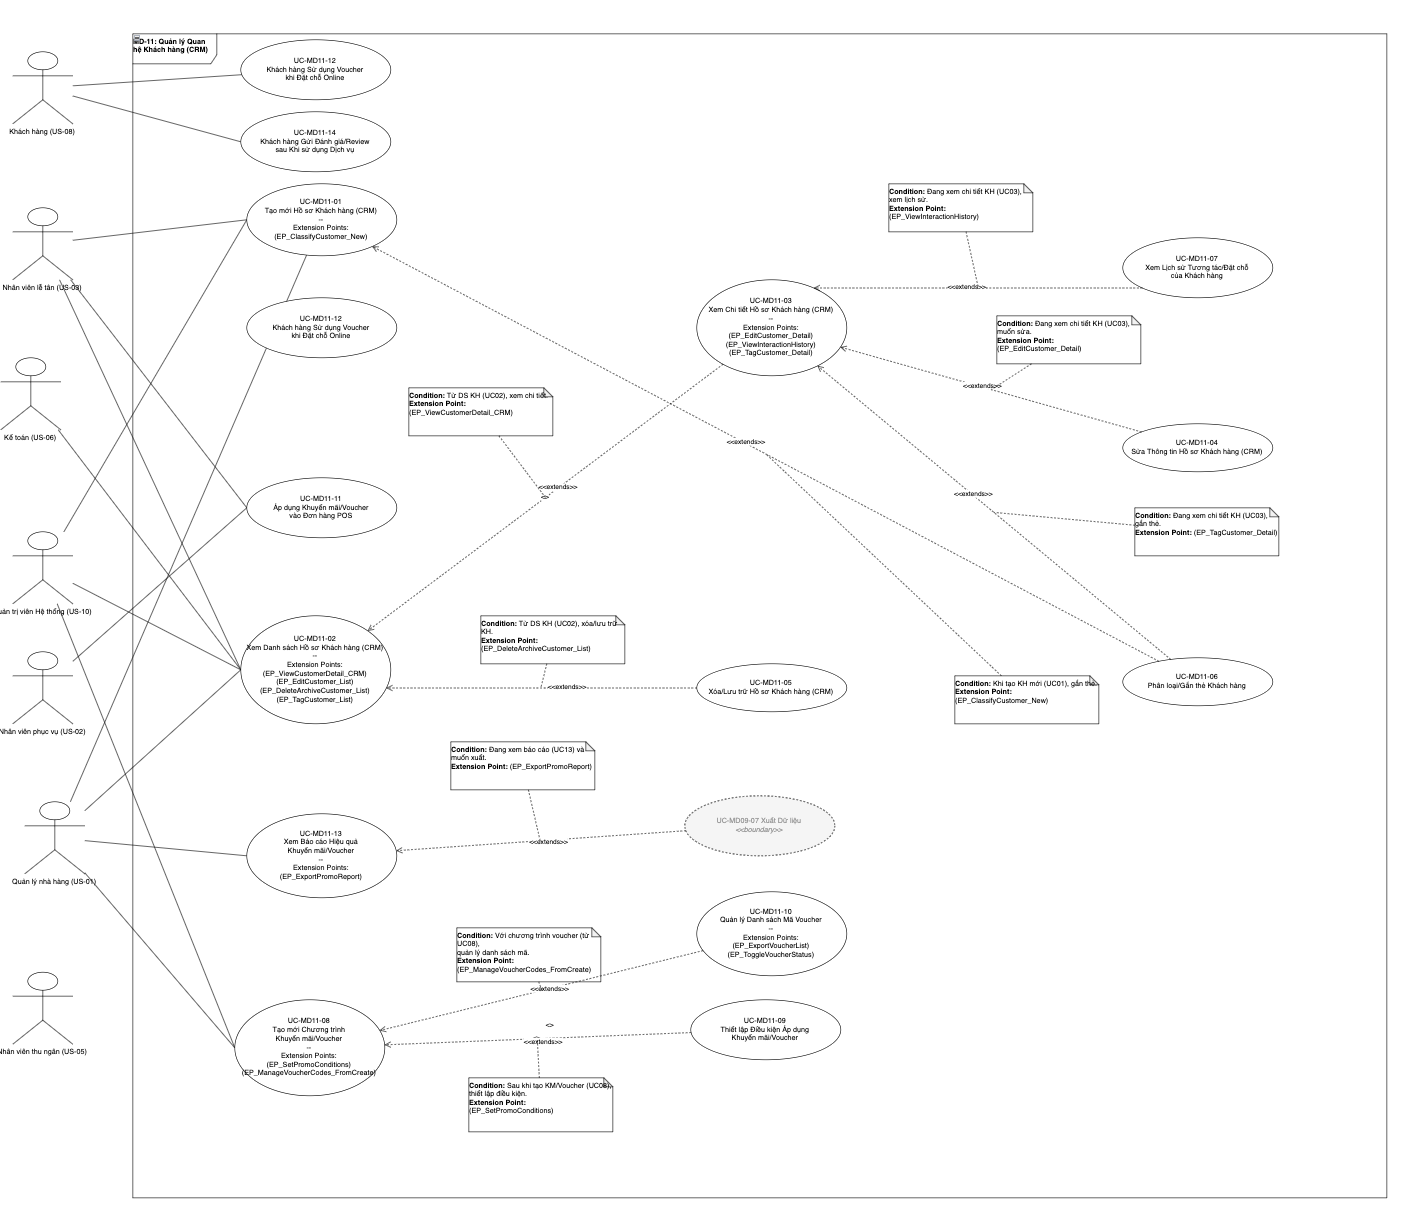
\includegraphics[width=15cm]{Sections/tong_quan/functional_spec/img/uc11.png}
    \vspace{0.5cm}
    \caption{Use case diagram cho Module MD-11}
    \label{fig:my_label}
\end{figure}

\begin{longtable}{|m{2cm}|m{2.5cm}|m{2.5cm}|m{4.5cm}|m{4cm}|}
\caption{Danh sách Yêu cầu Chức năng cho Module MD-11: Quản lý Quan hệ Khách hàng (CRM)} \label{tab:fr_md11_crm_marketing_revised_in_codeblock} \\
\hline
\textbf{Mã Module} & \textbf{Mã Yêu cầu CN} & \textbf{Mã Người dùng} & \textbf{Tên Chức năng} & \textbf{Mô tả Ngắn} \\
\hline
\endhead % Header cho các trang tiếp theo
\midrule
\endfoot % Footer cho bảng
\bottomrule
\endlastfoot % Footer cho trang cuối cùng

% === Quản lý Hồ sơ Khách hàng (CRM View) - Tách nhỏ ===
MD-11 & FR-MD11-01 & US-01, US-03, US-10 & Tạo mới Hồ sơ Khách hàng (CRM) & Nhân viên/Quản lý tạo hồ sơ mới cho khách hàng với các thông tin chi tiết. \\
\hline
MD-11 & FR-MD11-02 & US-01, US-03, US-10 & Xem Danh sách Hồ sơ Khách hàng (CRM) & Xem danh sách tất cả khách hàng trong hệ thống CRM, có thể tìm kiếm, lọc. \\
\hline
MD-11 & FR-MD11-03 & US-01, US-03, US-10 & Xem Chi tiết Hồ sơ Khách hàng (CRM) & Xem toàn bộ thông tin chi tiết của một khách hàng cụ thể (thông tin cá nhân, lịch sử, sở thích...). \\
\hline
MD-11 & FR-MD11-04 & US-01, US-03, US-10 & Sửa Thông tin Hồ sơ Khách hàng (CRM) & Cập nhật, chỉnh sửa các thông tin trong hồ sơ của một khách hàng đã có. \\
\hline
MD-11 & FR-MD11-05 & US-01, US-10 & Xóa/Lưu trữ Hồ sơ Khách hàng (CRM) & Xóa (nếu chưa có giao dịch) hoặc lưu trữ (ẩn đi) hồ sơ khách hàng không còn hoạt động. \\
\hline
MD-11 & FR-MD11-06 & US-01, US-06, US-10 & Phân loại/Gắn thẻ Khách hàng & Phân loại khách hàng (VIP, thường xuyên...) hoặc gắn thẻ (tag) cho khách hàng để phục vụ marketing, chăm sóc. \\
\hline
MD-11 & FR-MD11-07 & US-01, US-06, US-10 & Xem Lịch sử Tương tác/Đặt chỗ của Khách hàng & Truy cập toàn bộ lịch sử đặt chỗ, hóa đơn, phản hồi, ghi chú tương tác của một khách hàng cụ thể. \\
\hline

% === Quản lý Voucher/Khuyến mãi ===
MD-11 & FR-MD11-08 & US-01, US-10 & Tạo mới Chương trình Khuyến mãi/Voucher & Định nghĩa các chương trình khuyến mãi (giảm giá \%, giảm tiền cố định, mua X tặng Y) hoặc tạo mã voucher. \\
\hline
MD-11 & FR-MD11-09 & US-01, US-10 & Thiết lập Điều kiện Áp dụng Khuyến mãi/Voucher & Cấu hình điều kiện: thời gian, giá trị đơn tối thiểu, sản phẩm/danh mục áp dụng, số lần sử dụng... \\
\hline
MD-11 & FR-MD11-10 & US-01, US-10 & Quản lý Danh sách Mã Voucher & Xem danh sách mã voucher đã tạo, trạng thái (đã dùng, còn hạn), có thể xuất mã hàng loạt, vô hiệu hóa voucher. \\
\hline
MD-11 & FR-MD11-11 & US-02, US-05 & Áp dụng Khuyến mãi/Voucher vào Đơn hàng POS & Nhân viên POS nhập mã voucher hoặc chọn chương trình khuyến mãi đủ điều kiện để áp dụng cho đơn hàng. \\
\hline
MD-11 & FR-MD11-12 & US-08 & Khách hàng Sử dụng Voucher khi Đặt chỗ Online & Khách hàng nhập mã voucher hợp lệ vào đơn đặt chỗ/đặt món online để được giảm giá. \\
\hline
MD-11 & FR-MD11-13 & US-01 & Xem Báo cáo Hiệu quả Khuyến mãi/Voucher & Thống kê số lần sử dụng, tổng giá trị giảm giá của từng chương trình/voucher. (Mở rộng từ UC-MD09-09) \\
\hline

% === Thu thập & Quản lý Đánh giá/Phản hồi ===
MD-11 & FR-MD11-14 & US-08 & Khách hàng Gửi Đánh giá/Review sau Khi sử dụng Dịch vụ & Khách hàng (có thể qua email mời hoặc link trên hóa đơn) gửi đánh giá về chất lượng món ăn, dịch vụ. \\
\hline
MD-11 & FR-MD11-15 & US-01, US-09 & Xem và Quản lý Đánh giá/Phản hồi của Khách hàng & Quản lý xem các đánh giá, có thể phản hồi, phân loại (tích cực, tiêu cực), hoặc đánh dấu đã xử lý. \\
\hline
MD-11 & FR-MD11-16 & US-01 & (Tùy chọn) Hiển thị Đánh giá Tích cực trên Website & Chọn lọc và hiển thị các đánh giá tốt của khách hàng trên trang web nhà hàng (nếu muốn). \\
\hline
% Các chức năng khác như Loyalty, Email Marketing sẽ được thêm vào sau nếu cần
\end{longtable}

\subsubsubsection{Mục tiêu và Phạm vi}
\label{sssec:md11_objectives_scope}
Mục tiêu chính của module MD-11 là:
\begin{itemize}
    \item \textbf{Xây dựng cơ sở dữ liệu khách hàng toàn diện:} Lưu trữ thông tin liên hệ, lịch sử giao dịch, sở thích và các ghi chú quan trọng về từng khách hàng.
    \item \textbf{Phân loại và phân khúc khách hàng:} Cho phép gắn thẻ, phân loại khách hàng (ví dụ: VIP, khách thường xuyên) để phục vụ các chiến dịch chăm sóc và marketing cá nhân hóa.
    \item \textbf{Quản lý chương trình khuyến mãi và voucher hiệu quả:} Tạo, cấu hình điều kiện áp dụng, theo dõi việc sử dụng và đánh giá hiệu quả của các chương trình khuyến mãi và mã voucher.
    \item \textbf{Thu thập và quản lý phản hồi của khách hàng:} Cung cấp kênh cho khách hàng gửi đánh giá và cho phép nhà hàng xem xét, phân tích các phản hồi này.
    \item \textbf{Tăng cường tương tác và chăm sóc khách hàng:} Cung cấp thông tin để nhân viên có thể phục vụ khách hàng tốt hơn và xây dựng mối quan hệ lâu dài.
    \item \textbf{Hỗ trợ các hoạt động marketing:} Cung cấp dữ liệu khách hàng cho việc tạo các chiến dịch email marketing hoặc các hoạt động quảng bá khác (có thể tích hợp với module marketing riêng).
\end{itemize}
Phạm vi của module bao gồm việc quản lý hồ sơ khách hàng từ khi tạo mới, cập nhật thông tin, theo dõi lịch sử, cho đến việc thiết kế và quản lý các chương trình khuyến mãi/voucher, cũng như quy trình thu thập và xem xét đánh giá từ khách hàng.

\subsubsubsection{Đối tượng Sử dụng Chính}
\label{sssec:md11_primary_users}
Các đối tượng người dùng chính tương tác với module này bao gồm:
\begin{itemize}
    \item \textbf{US-01 (Quản lý nhà hàng):} Là người dùng chính, chịu trách nhiệm tạo và quản lý các chương trình khuyến mãi, xem báo cáo hiệu quả, quản lý hồ sơ khách hàng VIP, và xem xét các đánh giá của khách hàng.
    \item \textbf{US-03 (Nhân viên lễ tân):} Thường xuyên tạo mới và cập nhật hồ sơ khách hàng, có thể xem lịch sử đặt chỗ của khách để hỗ trợ tốt hơn.
    \item \textbf{US-06 (Kế toán):} Có thể cần xem thông tin khách hàng liên quan đến hóa đơn hoặc các chương trình khách hàng thân thiết.
    \item \textbf{US-10 (Quản trị viên Hệ thống):} Có thể tham gia vào việc cấu hình ban đầu của module CRM, tạo các trường tùy chỉnh hoặc thiết lập các quy tắc tự động (nếu có).
    \item \textbf{US-08 (Khách hàng):} Là người cung cấp thông tin cá nhân, sử dụng voucher khi đặt chỗ online, và gửi đánh giá/review về dịch vụ.
    \item \textbf{US-02 (Nhân viên phục vụ) / US-05 (Nhân viên thu ngân):} Áp dụng các chương trình khuyến mãi hoặc mã voucher cho đơn hàng tại POS.
\end{itemize}

\subsubsubsection{Các Chức năng Chính}
\label{sssec:md11_key_functionalities}
Module MD-11 cung cấp một bộ các chức năng tập trung vào việc quản lý và tăng cường mối quan hệ với khách hàng:

\begin{itemize}
    \item \textbf{Quản lý Hồ sơ Khách hàng (UC-MD11-01 đến UC-MD11-07):}
    \begin{itemize}
        \item Tạo mới một hồ sơ khách hàng trong hệ thống CRM với các thông tin liên hệ cơ bản (UC-MD11-01).
        \item Xem danh sách tất cả các hồ sơ khách hàng với khả năng tìm kiếm và lọc (UC-MD11-02).
        \item Xem thông tin chi tiết đầy đủ của một hồ sơ khách hàng, bao gồm lịch sử giao dịch và tương tác (UC-MD11-03).
        \item Sửa đổi và cập nhật các thông tin trong một hồ sơ khách hàng đã tồn tại (UC-MD11-04).
        \item Xóa vĩnh viễn (nếu không có giao dịch) hoặc lưu trữ (ẩn đi) các hồ sơ khách hàng không còn phù hợp (UC-MD11-05).
        \item Gán các thẻ (tags) hoặc phân loại khách hàng (ví dụ: VIP, Thường xuyên) để phục vụ việc nhóm và phân tích (UC-MD11-06).
        \item Truy cập và xem lại toàn bộ lịch sử các hoạt động và giao dịch liên quan đến một khách hàng cụ thể (UC-MD11-07).
    \end{itemize}

    \item \textbf{Quản lý Chương trình Khuyến mãi và Voucher (UC-MD11-08 đến UC-MD11-13):}
    \begin{itemize}
        \item Định nghĩa một chương trình khuyến mãi mới hoặc một lô mã voucher mới, bao gồm loại hình và giá trị khuyến mãi (UC-MD11-08).
        \item Thiết lập các điều kiện và quy tắc chi tiết để chương trình/voucher có thể được áp dụng (ví dụ: thời gian hiệu lực, giá trị đơn hàng tối thiểu, sản phẩm áp dụng) (UC-MD11-09).
        \item Xem danh sách các mã voucher đã tạo, kiểm tra trạng thái, và có thể thực hiện xuất file hoặc vô hiệu hóa mã (UC-MD11-10).
        \item Nhân viên tại POS áp dụng một chương trình khuyến mãi hoặc nhập mã voucher hợp lệ vào đơn hàng của khách (UC-MD11-11).
        \item Khách hàng tự nhập và sử dụng mã voucher hợp lệ khi thực hiện đặt chỗ hoặc đặt món trước trực tuyến (UC-MD11-12).
        \item Xem báo cáo thống kê chi tiết về tình hình sử dụng và hiệu quả của các chương trình khuyến mãi hoặc voucher (UC-MD11-13).
    \end{itemize}

    \item \textbf{Quản lý Đánh giá và Phản hồi từ Khách hàng (UC-MD11-14, và sẽ có các UC tiếp theo như UC-MD11-15, UC-MD11-16):}
    \begin{itemize}
        \item Cho phép khách hàng gửi các ý kiến đánh giá, nhận xét, hoặc xếp hạng về dịch vụ của nhà hàng thông qua các kênh trực tuyến (UC-MD11-14).
        \item (Dự kiến) Cho phép Quản lý nhà hàng xem danh sách các đánh giá đã nhận được.
        \item (Dự kiến) Cho phép Quản lý nhà hàng xem chi tiết một đánh giá cụ thể và có thể thực hiện các hành động phản hồi.
    \end{itemize}
\end{itemize}

\subsubsubsection{Tóm tắt Luồng Hoạt động Tổng thể}
\label{sssec:md11_overall_workflow}
Luồng hoạt động trong module Quản lý Quan hệ Khách hàng (CRM) thường bao gồm các giai đoạn và quy trình sau:
\begin{enumerate}
    \item \textbf{Thu thập và Quản lý Thông tin Khách hàng:}
        \begin{itemize}
            \item Nhân viên Tạo mới Hồ sơ Khách hàng (CRM) (UC-MD11-01) khi có khách mới hoặc nhập dữ liệu.
            \item Nhân viên thường xuyên Xem Danh sách Hồ sơ Khách hàng (UC-MD11-02), Xem Chi tiết Hồ sơ Khách hàng (UC-MD11-03) để tra cứu, và Sửa Thông tin Hồ sơ Khách hàng (UC-MD11-04) khi cần cập nhật.
            \item Thực hiện Phân loại/Gắn thẻ Khách hàng (UC-MD11-06) để phục vụ các mục đích khác nhau.
            \item Khi cần, Xóa/Lưu trữ Hồ sơ Khách hàng (CRM) (UC-MD11-05).
            \item Xem Lịch sử Tương tác/Đặt chỗ của Khách hàng (UC-MD11-07) để hiểu rõ hơn về khách.
        \end{itemize}
    \item \textbf{Triển khai và Quản lý Chương trình Khuyến mãi/Voucher:}
        \begin{itemize}
            \item Quản lý Tạo mới Chương trình Khuyến mãi/Voucher (UC-MD11-08).
            \item Thiết lập Điều kiện Áp dụng Khuyến mãi/Voucher (UC-MD11-09) chi tiết cho từng chương trình.
            \item (Nếu là voucher) Quản lý Danh sách Mã Voucher (UC-MD11-10), có thể xuất file hoặc vô hiệu hóa mã.
            \item Nhân viên tại POS Áp dụng Khuyến mãi/Voucher vào Đơn hàng POS (UC-MD11-11) cho khách.
            \item Khách hàng Sử dụng Voucher khi Đặt chỗ Online (UC-MD11-12) trên website/app.
            \item Quản lý định kỳ Xem Báo cáo Hiệu quả Khuyến mãi/Voucher (UC-MD11-13) để đánh giá.
        \end{itemize}
    \item \textbf{Thu thập và Xử lý Phản hồi Khách hàng:}
        \begin{itemize}
            \item Khách hàng Gửi Đánh giá/Review sau Khi sử dụng Dịch vụ (UC-MD11-14).
            \item (Dự kiến) Quản lý xem xét các đánh giá này và có thể phản hồi hoặc thực hiện các hành động cải thiện dịch vụ.
        \end{itemize}
\end{enumerate}
Module MD-11 giúp nhà hàng không chỉ quản lý giao dịch mà còn xây dựng mối quan hệ ý nghĩa với khách hàng, từ đó tạo lợi thế cạnh tranh và phát triển bền vững.




% \subsection{Yêu cầu chất lương}

% % \subsubsection{Yêu cầu chức năng}

% Trong phạm vi đồ án này, chúng em sẽ tập trung vào các đối tượng chính sử dụng hệ thống, bao gồm Khách hàng, Nhân viên phục vụ, Nhân viên thu ngân, Nhân viên chăm sóc khách hàng, Nhân viên bếp, Quản lý chi nhánh và Quản lý tổng, nhằm đảm bảo hệ thống đáp ứng tốt nhu cầu vận hành và trải nghiệm của từng vai trò.

% \begin{figure}[H]
%     \centering
%     \includegraphics[width=15cm]{Images/nguoi-dung-he-thong.png}
%     \vspace{0.5cm}
%     \caption{Các đối tượng người dùng của hệ thống}
%     \label{fig:my_label}
% \end{figure}

% \textbf{Đối với Khách hàng}
% \begin{itemize}
%     \item Đăng ký, đăng nhập
%     \item Gửi yêu cầu đặt bàn trực tuyến, xem được tổng quan vị trí, trạng thái bàn thông qua các sơ đồ
%     \item Hủy yêu cầu đặt bàn cho đến khi trước thời gian hẹn 2 tiếng
%     \item Quét QR để truy cập vào menu và đặt món, không cần gọi nhân viên
%     \item Xem danh sách món ăn và đồ uống, kèm theo hình ảnh, mô tả và giá cả
%     \item Tìm kiếm món ăn theo tên hoặc danh mục, giá cả
%     \item Chọn món, số lượng và tùy chọn (size, topping, gia vị)
%     \item Gợi ý món ăn phù hợp dựa trên lịch sử đơn hàng và số liệu phân tích
%     \item Thêm món vào giỏ hàng
%     \item Xem lại giỏ hàng trước khi xác nhận đặt món
%     \item Đặt món nhiều lần trong cùng một lượt sử dụng tại nhà hàng, để có thể thay đổi món ăn trong suốt quá trình ăn
%     \item Gửi yêu cầu hủy đơn hoặc hủy/thay đổi các món cụ thể
%     \item Xem lại các đơn hàng đã đặt trước đó
%     \item Xem chi tiết các món đã đặt, tổng tiền và các khuyến mãi (nếu có)
%     \item Gửi yêu cầu thanh toán bằng cách quét mã QR, hoặc thao tác trên ứng dụng
%     \item Nhận thông báo về các khuyến mãi và ưu đãi
%     \item Gửi phản hồi về món ăn hoặc dịch vụ
%     \item Gửi khiếu nại nếu có sự cố
%     \item Trò chuyện trực tiếp với nhân viên chăm sóc khách hàng
% \end{itemize}

% \textbf{Đối với Phục vụ}
% \begin{itemize}
%     \item Xem danh sách trạng thái bàn
%     \item Hỗ trợ khách hàng đặt món, thanh toán
%     \item Xem danh sách đơn hàng của khách
%     \item Nhận thông báo khi món ăn đã sẵn sàng
%     \item Xử lý yêu cầu hủy đơn hoặc hủy/thay đổi món của khách
%     \item Chuyển vị trí đơn hàng sang bàn khác.
%     \item Đặt lại trạng thái bàn
% \end{itemize}

% \textbf{Đối với Thu ngân}
% \begin{itemize}
%     \item Nhận thông báo khi có yêu cầu thanh toán
%     \item Xem chi tiết đơn hàng và tổng hóa đơn
%     \item Áp dụng khuyến mãi và giảm giá khi thanh toán
%     \item Quản lý các phương thức thanh toán
%     \item Nhận thông báo về thanh toán thành công với phương thức quét QR, quẹt thẻ
%     \item Cập nhật trạng thái thanh toán với phương thức thanh toán tiền mặt
%     \item In hóa đơn cho khách hàng
%     \item Xử lý yêu cầu hoàn tiền (vấn đề phát sinh)
%     \item Tạo báo cáo doanh thu hàng ngày
% \end{itemize}

% \textbf{Đối với Nhân viên chăm sóc khách hàng}
% \begin{itemize}
%     \item Tiếp nhận và xử lý yêu cầu từ khách hàng
%     \item Theo dõi và quản lý khiếu nại \& phản hồi từ khách hàng
%     \item Trả lời tin nhắn trực tuyến với khách hàng
%     \item Cập nhật thông tin khách hàng
%     \item Theo dõi và nhắc nhở khách hàng về các chương trình ưu đãi qua tài khoản và email
% \end{itemize}

% \textbf{Đối với Nhân viên bếp}
% \begin{itemize}
%     \item Nhận đơn hàng từ hệ thống quản lý đơn hàng
%     \item Xem tất cả danh sách món ăn được sắp xếp theo thứ tự ưu tiên
%     \item Xem được các yêu cầu đặc biệt của từng món ăn cần làm
%     \item Cập nhật trạng thái chế biến của từng món ăn (chưa làm, đang chế biến, hoàn thành...)
% \end{itemize}

% \textbf{Đối với Quản lý chi nhánh}
% \begin{itemize}
%     \item Thêm/Chỉnh sửa sơ đồ nhà hàng
%     \item Xử lý, xác nhận các yêu cầu đặt bàn của khách hàng tại chi nhánh
%     \item Xem báo cáo kinh doanh và doanh thu của chi nhánh
%     \item Điều chỉnh và thiết lập các chương trình khuyến mãi, marketing chi nhánh
%     \item Theo dõi các phản hồi của khách hàng
%     \item Xem danh sách nhân viên
%     \item Phân chia công việc cho các tài khoản nhân viên
% \end{itemize}

% \textbf{Đối với Quản lý tổng}
% \begin{itemize}
%     \item Quản lý thông tin chi nhánh
%     \item Thêm/Xóa chi nhánh
%     \item Quản lý các tài khoản nhân viên và khách hàng
%     \item Xem báo cáo tổng quan tất cả các chi nhánh
%     \item Xem báo cáo chi tiết của một chi nhánh tổng
% \end{itemize}

% % User Story là một kỹ thuật phát triển phần mềm tập trung vào nhu cầu của người dùng trong quá trình sử dụng sản phẩm. Mục đích của User Story là giúp các nhà phát triển phần mềm hiểu rõ những tính năng cốt lõi của sản phẩm và xác định được các chức năng cần thiết để hiện thực đầu tiên của ứng dụng.\\

% % Để đưa ra danh sách User Story của ứng dụng, nhóm chúng em đã tiến hành thảo luận, nghiên cứu và phân tích yêu cầu của người dùng. Chúng tôi bắt đầu xây dựng hệ thống tuyển dụng bằng cách xác định các tính năng cơ bản cần phải có trong ứng dụng để đáp ứng nhu cầu và mong muốn của người dùng.\\

% % \textbf{Một số user story cơ bản như sau:}
% % \begin{itemize}
% %     \item Đối với Khách hàng
% %     \begin{enumerate}
% %         \item Là Khách Hàng, tôi muốn quét mã QR trên bàn để truy cập vào menu và đặt món.
% %         \item Là Khách Hàng, tôi muốn xem danh sách các món ăn và đồ uống, kèm theo hình ảnh, mô tả và giá cả.
% %         \item Là Khách Hàng, tôi muốn tìm kiếm món ăn theo tên hoặc danh mục.
% %         \item Là Khách Hàng, tôi muốn chọn món, số lượng và các tùy chọn (ví dụ: size, topping, gia vị).
% %         \item Là Khách Hàng, tôi muốn thêm các món đã chọn vào giỏ hàng.
% %         \item Là Khách Hàng, tôi muốn xem lại giỏ hàng trước khi xác nhận đặt món.
% %         \item Là Khách Hàng, tôi muốn đặt món nhiều lần trong cùng một lượt sử dụng tại nhà hàng.
% %         \item Là Khách Hàng, tôi muốn xem lại các order đã đặt trước đó (nếu đã đăng nhập).
% %         \item Là Khách Hàng, tôi muốn xem chi tiết các món đã đặt, tổng tiền và các khuyến mãi (nếu có).
% %         \item Là Khách Hàng, tôi muốn thanh toán bằng cách quét mã QR hoặc thanh toán tiền mặt.
% %         \item Là Khách Hàng, tôi muốn xem lại hóa đơn sau khi đã thanh toán.
% %         \item Là Khách Hàng, tôi muốn đăng ký tài khoản thành viên để tham gia chương trình khách hàng thân thiết.
% %         \item Là Khách Hàng, tôi muốn đăng nhập để xem lịch sử đặt món, nhận khuyến mãi và các ưu đãi khác.
% %     \end{enumerate}
% %     \item Đối với Nhân Viên Thu Ngân/Phục Vụ
% %     \begin{enumerate}
% %         \item Là Nhân Viên Thu Ngân/Phục Vụ, tôi muốn xem danh sách các order mới và đang chờ xử lý.
% %         \item Là Nhân Viên Thu Ngân/Phục Vụ, tôi muốn xem chi tiết các order của khách hàng.
% %         \item Là Nhân Viên Thu Ngân/Phục Vụ, tôi muốn gộp các order của một bàn thành một hóa đơn duy nhất.
% %         \item Là Nhân Viên Thu Ngân/Phục Vụ, tôi muốn xóa bỏ các order nếu cần.
% %         \item Là Nhân Viên Thu Ngân/Phục Vụ, tôi muốn xác nhận thanh toán bằng QR.
% %         \item Là Nhân Viên Thu Ngân/Phục Vụ, tôi muốn xác nhận thanh toán bằng tiền mặt (tự thao tác).
% %         \item Là Nhân Viên Thu Ngân/Phục Vụ, tôi muốn in hóa đơn cho khách hàng (có mã QR để thanh toán).
% %         \item Là Nhân Viên Thu Ngân/Phục Vụ, tôi muốn check-in (chấm công) đầu ca và check-out (chấm công) cuối ca.
% %         \item Là Nhân Viên Thu Ngân/Phục Vụ, tôi muốn chuyển order từ bàn này sang bàn khác (nếu khách hàng muốn đổi bàn).
% %     \end{enumerate}
% %     \item Đối với Quản Lý Chi Nhánh
% %     \begin{enumerate}
% %         \item Là Quản Lý Chi Nhánh, tôi muốn nhập kho, xem danh sách các nguyên liệu trong kho.
% %         \item Là Quản Lý Chi Nhánh, tôi muốn theo dõi số lượng còn lại của từng nguyên liệu.
% %         \item Là Quản Lý Chi Nhánh, tôi muốn xem báo cáo nhập/xuất kho hàng ngày.
% %         \item Là Quản Lý Chi Nhánh, tôi muốn xem danh sách nhân viên.
% %         \item Là Quản Lý Chi Nhánh, tôi muốn phân công ca làm cho nhân viên.
% %         \item Là Quản Lý Chi Nhánh, tôi muốn xem lịch sử check-in/check-out của nhân viên.
% %         \item Là Quản Lý Chi Nhánh, tôi muốn xem các báo cáo về doanh thu và số lượng món ăn bán được trong chi nhánh.
% %         \item Là Quản Lý Chi Nhánh, tôi muốn xem các báo cáo về kho nguyên liệu.
% %         \item Là Quản Lý Chi Nhánh, tôi muốn xem danh sách bàn đang có.
% %         \item Là Quản Lý Chi Nhánh, tôi muốn sắp xếp bàn cho khách hàng và quản lý bàn trống.
% %     \end{enumerate}
% %     \item Đối với Quản Lý Tổng
% %     \begin{enumerate}
% %         \item Là Quản Lý Tổng, tôi muốn xem tổng doanh thu của tất cả các chi nhánh.
% %         \item Là Quản Lý Tổng, tôi muốn xem chi tiết doanh thu của từng chi nhánh, theo ngày, tuần, tháng, năm.
% %         \item Là Quản Lý Tổng, tôi muốn xem các báo cáo tổng quan về hoạt động của nhà hàng.
% %         \item Là Quản Lý Tổng, tôi muốn xuất báo cáo tổng quan về doanh thu, chi phí và lợi nhuận.
% %         \item Là Quản Lý Tổng, tôi muốn xem danh sách tất cả các chi nhánh.
% %         \item Là Quản Lý Tổng, tôi muốn thêm, sửa hoặc xóa thông tin chi nhánh.
% %         \item Là Quản Lý Tổng, tôi muốn xem các báo cáo tổng quan từ các chi nhánh.
% %         \item Là Quản Lý Tổng, tôi muốn thêm, chỉnh sửa hoặc xóa các món ăn và đồ uống trong thực đơn.
% %         \item Là Quản Lý Tổng, tôi muốn thay đổi giá cả, mô tả và hình ảnh của món ăn.
% %     \end{enumerate}
% %     \item Các Tính Năng Mở Rộng (Optional)
% %     \begin{enumerate}
% %         \item Là Khách Hàng, tôi muốn hệ thống gợi ý món ăn dựa trên lịch sử đặt món của mình.
% %         \item Là Quản Lý (Tổng/Chi Nhánh), tôi muốn tạo và quản lý các chương trình khuyến mãi, giảm giá.
% %         \item Là Khách Hàng, tôi muốn đặt bàn trước thông qua ứng dụng.
% %         \item Là Khách Hàng, tôi muốn đánh giá chất lượng món ăn và dịch vụ của nhà hàng.
% %         \item Là Quản Lý (Tổng/Chi Nhánh), tôi muốn hệ thống tự động xuất dữ liệu sang hệ thống kế toán.
% %     \end{enumerate}
% % \end{itemize}

% % \textbf{Một số usecase diagram cơ bản như sau:}

% % \begin{figure}[H]
% %     \centering
% %     \includegraphics[width=15cm]{Images/us-dat-mon.png}
% %     \vspace{0.5cm}
% %     \caption{Các use case liên quan đến đặt món}
% %     \label{fig:my_label}
% % \end{figure}

% % \begin{figure}[H]
% %     \centering
% %     \includegraphics[width=15cm]{Images/us-tai-khoan.png}
% %     \vspace{0.5cm}
% %     \caption{Các use case liên quan đến quản lý tài khoản}
% %     \label{fig:my_label}
% % \end{figure}

% % \begin{figure}[H]
% %     \centering
% %     \includegraphics[width=15cm]{Images/us-quan-ly.png}
% %     \vspace{0.5cm}
% %     \caption{Các use case liên quan đến quản lý}
% %     \label{fig:my_label}
% % \end{figure}

% % \begin{enumerate}[(a)]
% %     \item Khách hàng
% %     \begin{itemize}
% %         \item Quét mã QR
% %         \begin{itemize}
% %             \item Khách hàng quét mã QR trên bàn để truy cập vào menu và đặt món.
% %         \end{itemize}
% %         \item Xem menu
% %         \begin{itemize}
% %             \item Xem danh sách các món ăn và đồ uống, kèm theo hình ảnh, mô tả, giá cả.
% %             \item Tìm kiếm món ăn theo tên hoặc danh mục.
% %         \end{itemize}
% %         \item Đặt món
% %         \begin{itemize}
% %             \item Chọn món, số lượng, tùy chọn (ví dụ: size, topping, gia vị)
% %             \item Thêm món vào giỏ hàng.
% %             \item Xem lại giỏ hàng trước khi xác nhận đặt món.
% %             \item Đặt món nhiều lần trong cùng một lượt sử dụng.
% %         \end{itemize}
% %         \item Xem lịch sử đặt món
% %         \begin{itemize}
% %             \item Xem lại các order đã đặt trước đó (nếu đã đăng nhập).
% %         \end{itemize}
% %         \item Xem hóa đơn
% %         \begin{itemize}
% %             \item Xem chi tiết các món đã đặt, tổng tiền, các khuyến mãi (nếu có).
% %         \end{itemize}
% %         \item Thanh toán
% %         \begin{itemize}
% %             \item Thanh toán bằng cách quét mã QR hoặc thanh toán tiền mặt.
% %             \item Xem lại hóa đơn sau khi đã thanh toán.
% %         \end{itemize}
% %         \item Đăng ký/Đăng nhập (Tùy chọn)
% %         \begin{itemize}
% %             \item Đăng ký tài khoản thành viên để tham gia chương trình khách hàng thân thiết.
% %             \item Đăng nhập để xem lịch sử đặt món, nhận khuyến mãi và các ưu đãi khác.
% %         \end{itemize}
% %     \end{itemize}
% %     \item Nhân viên thu ngân/phục vụ
% %     \begin{itemize}
% %         \item Quản lý order
% %         \begin{itemize}
% %             \item Xem danh sách các order mới và đang chờ xử lý.
% %             \item Xem chi tiết các order của khách hàng.
% %         \end{itemize}
% %         \item Gộp hóa đơn
% %         \begin{itemize}
% %             \item Gộp các order của một bàn thành một hóa đơn duy nhất.
% %             \item Xóa bỏ các order (nếu cần)
% %         \end{itemize}
% %         \item Xác nhận thanh toán
% %         \begin{itemize}
% %             \item Xác nhận thanh toán bằng QR.
% %             \item Xác nhận thanh toán bằng tiền mặt (tự thao tác).
% %         \end{itemize}
% %         \item In hóa đơn
% %         \begin{itemize}
% %             \item In hóa đơn cho khách hàng (có mã QR để thanh toán).
% %         \end{itemize}
% %         \item Check-in/Check-out
% %         \begin{itemize}
% %             \item Chấm công đầu ca và cuối ca.
% %         \end{itemize}
% %         \item Chuyển Order
% %         \begin{itemize}
% %             \item Có thể chuyển order từ bàn này sang bàn khác (nếu khách hàng muốn đổi bàn)
% %         \end{itemize}
% %     \end{itemize}
% %     \item Chức năng cho quản lý chi nhánh
% %     \begin{itemize}
% %         \item Quản lý kho nguyên liệu
% %         \begin{itemize}
% %             \item Nhập kho, xem danh sách các nguyên liệu trong kho.
% %             \item Theo dõi số lượng còn lại của từng nguyên liệu.
% %             \item Báo cáo nhập/xuất kho hàng ngày.
% %         \end{itemize}
% %         \item Quản lý nhân viên
% %         \begin{itemize}
% %             \item Xem danh sách nhân viên.
% %             \item Phân công ca làm.
% %             \item Xem lịch sử check-in/check-out của nhân viên.
% %         \end{itemize}
% %         \item Xem báo cáo
% %         \begin{itemize}
% %             \item Xem các báo cáo về doanh thu, số lượng món ăn bán được trong chi nhánh.
% %             \item Xem các báo cáo về kho nguyên liệu.
% %         \end{itemize}
% %         \item Quản lý bàn
% %         \begin{itemize}
% %             \item Xem danh sách bàn đang có.
% %             \item Có thể sắp xếp bàn cho khách hàng, quản lý bàn trống.
% %         \end{itemize}
% %     \end{itemize}
% %     \item Chức năng cho quản lý tổng
% %     \begin{itemize}
% %         \item Quản lý doanh thu
% %         \begin{itemize}
% %             \item Xem tổng doanh thu của tất cả các chi nhánh.
% %             \item Xem chi tiết doanh thu của từng chi nhánh, theo ngày, tuần, tháng, năm.
% %         \end{itemize}
% %         \item Xem báo cáo
% %         \begin{itemize}
% %             \item Xem các báo cáo tổng quan về hoạt động của nhà hàng.
% %             \item Xuất báo cáo tổng quan về doanh thu, chi phí, lợi nhuận.
% %         \end{itemize}
% %         \item Quản lý chi nhánh
% %         \begin{itemize}
% %             \item Xem danh sách tất cả các chi nhánh.
% %             \item Thêm/sửa/xóa thông tin chi nhánh.
% %             \item Xem các báo cáo tổng quan từ các chi nhánh.
% %         \end{itemize}
% %         \item Quản lý thực đơn
% %         \begin{itemize}
% %             \item Thêm, chỉnh sửa, xóa các món ăn và đồ uống trong thực đơn.
% %             \item Thay đổi giá cả, mô tả, hình ảnh của món ăn.
% %         \end{itemize}
% %     \end{itemize}
% %     \item Mở rộng (có thể làm nếu kịp thời gian)
% %     \begin{itemize}
% %         \item Hệ thống gợi ý món ăn: Dựa trên lịch sử đặt món của khách hàng, hệ thống có thể gợi ý các món ăn phù hợp.
% %         \item Hệ thống quản lý khuyến mãi: Cho phép tạo và quản lý các chương trình khuyến mãi, giảm giá.
% %         \item Hệ thống đặt bàn: Cho phép khách hàng đặt bàn trước thông qua ứng dụng.
% %         \item Hệ thống quản lý đánh giá: Cho phép khách hàng đánh giá chất lượng món ăn và dịch vụ của nhà hàng.
% %         \item Tích hợp với hệ thống kế toán: Tự động xuất dữ liệu sang hệ thống kế toán.
% %     \end{itemize}
% % \end{enumerate}

% \subsubsection{Yêu cầu phi chức năng}
% \begin{itemize}
%     \item Bảo mật:
%     \begin{itemize}
%         \item Dữ liệu người dùng và dữ liệu giao dịch phải được bảo vệ.
%         \item Hệ thống sử dụng HTTPS để đảm bảo an toàn cho quá trình truyền dữ liệu.
%     \end{itemize}

%     \item Hiệu năng:
%     \begin{itemize}
%         \item Hệ thống phải có tốc độ xử lý nhanh và ổn định.
%         \item Khả năng đáp ứng nhanh chóng khi nhiều người dùng truy cập cùng một lúc.    
%     \end{itemize}

%     \item Tính khả dụng:
%     \begin{itemize}
%         \item Hệ thống hoạt động ổn định và có thời gian uptime cao.
%         \item Giao diện thân thiện và dễ sử dụng trên cả web và mobile.
%     \end{itemize}

%     \item Khả năng mở rộng:
%     \begin{itemize}
%         \item Hệ thống có thể mở rộng để hỗ trợ thêm nhiều chi nhánh và người dùng.
%         \item Dễ dàng thêm các tính năng mới khi cần thiết.
%     \end{itemize}

% \end{itemize}











